% Do not forget to include Introduction
%---------------------------------------------------------------
% \chapter{Introduction}
% uncomment the following line to create an unnumbered chapter
\chapter*{Introduction}\addcontentsline{toc}{chapter}{Introduction}\markboth{Introduction}{Introduction}
%---------------------------------------------------------------
\setcounter{page}{1}
S tím, jak se obchodování za poslední desetiletí stalo dostupnější, vyrostl i zájem o něj.
Pokud jde o obchodování, existují různé přístupy, někteří lidé nakupují aktiva pouze dlouhodobě, jiní se snaží obchodovat častěji, aby zvýšili své zisky.
S cílem činit chytrá rozhodnutí bez emocí a s konzistentními zisky, bylo vytvořeno algoritmické obchodování.

Algoritmické obchodní strategie jsou počítačové programy, které rozhodují o tom, kdy koupit nebo prodat na základě definovaných podmínek.
Nejsou svázáni stejnými omezeními jako lidé, necítí únavu a nenechají se svést emocemi.
Ve srovnání s lidskými obchodníky je lze předem vyhodnotit na historických datech.
Proces vyhodnocení se nazývá zpětné testování.

Strategie jsou většinou parametrizované a hledání optimálních parametrů je NP-těžký problém.
Předpokládá se, že neexistuje žádný účinný deterministický algoritmus, který by problém vyřešil v polynomiálním čase.
Algoritmus hrubé síly je užitečný pouze pro malou množinu hodnot možných parametrů, ale ve skutečnosti je většinou nepoužitelný, protože nenajde řešení v dostatečně krátkém čase.

Použití heuristiky se zdá být přirozeným přístupem.
I když se to ví už dlouho, stále to není standardní způsob optimalizace strategií.
Algoritmus hrubé síly lze zkušeným obchodníkům vysvětlit poměrně jednoduše, avšak pro pochopení heuristiky je zapotřebí mnohem hlubší úrovně porozumění.
Dalším důležitým aspektem je, že tvorba obecných generátorů vyhledávacího prostoru, které by generovaly platné konfigurace, je poměrně obtížné, jelikož existuje velké množství různých strategií.

Cílem této práce je implementovat vybranou algoritmickou obchodní strategii a pomocí heuristických přístupů spolehlivě a rychle najít její optimální parametry.
V rámci toho získat lepší porozumění algoritmickému obchodování a více zkušeností s implementací, používáním a laděním heuristik.
Ideálně vytvořit dobrý základ pro budoucí práci.

% popsat optimalizační kritérium
\chapter{Kombinatorická optimalizace}
Cílem řešení \textit{optimalizačního problému} je nalézt nejlepší řešení.
Formálně lze problém zapsat jako $P=(S, f, \Omega)$, kde $P$ je optimalizační problém, $S$ je vyhledávací prostor, $f$ je objektivní funkce a $\Omega$ je sada optimalizačních omezení.
Objektivní funkce je také označována jako cenová nebo fitness funkce.
Funkce slouží k hodnocení konfigurace a její hodnota slouží k jejich porovnání \cite{peres}.

Problémy lze dělit na minimalizační a maximalizační podle toho, zda je cílem maximalizovat nebo minimalizovat hodnotu objektivní funkce.
Vyhledávací prostor se skládá ze sady proměnných označovaných jako rozhodovací proměnné.
Pro získání platných řešení mohou být použita omezení \cite{kirkpatrik, peres}.

\textit{Kombinatorické optimalizační problémy} jsou definované pomocí diskrétních rozhodovacích proměnných.
Jelikož je množina přeskupení těchto proměnných konečná, je konečná i množina řešení.
Tyto problémy obvykle spadají do kategorie \textit{NP-těžkých} problémů \cite{peres}.

Obecně lze  kombinatorické problémy řešit pomocí \textit{hrubé síly}, která prohledá všechny možné řešení v prohledávacím prostoru \cite{peres}.
Největší výhodou tohoto přístupu je, že zaručuje nalezení nejlepšího možného řešení, nicméně je v praxi většinou nepoužitelný, jelikož neskončí v dostatečně krátkém čase \cite{efficient-backtesting}.
Konfigurace mohou být reprezentovány různými datovými strukturami, mezi nejběžnější patří: pole a stromy.
Typ kódování závisí na problému \cite{peres}.

\section{Třídy složitosti}
Obtížnost problému lze měřit pomocí \textit{výpočetní složitosti}, která se vztahuje k době, kterou algoritmus potřebuje k získání výsledku v závislosti na velikosti vstupu.
Výhodou je, že je nezávislá na hardwaru a umožňuje srovnání algoritmů \cite{peres}.

Problémy lze podle efektivity jejich řešení rozdělit do tříd.
Pokud je doba jejich běhu vázána na polynomiální funkci: $O(n^c)$, kde $c$ je nějaká konstanta a $n$ je velikost vstupu, jsou považovány za efektivní.
Ne všechny problémy však lze efektivně vyřešit.
Pokud problém patří do třídy \textit{NP-těžký}, je domníváno, že neexistuje žádný efektivní algoritmus k jeho řešení \cite{erickson}.

Rozhodovací problémy, jejichž výstupem je booleanovská hodnota, lze zařadit do 3 tříd.
Do třídy \textit{P} patří problémy, které lze vyřešit v polynomiálním čase.
Pokud lze odpověď \textit{ano} na problém ověřit v polynomiálním čase, patří do třídy \textit{NP}, což znamená nedeterministický polynomiální.
Pokud lze odpověď \textit{ne} ověřit v polynomiálním čase, tak patří do třídy \textit{co-NP}, která je komplementární třídě NP.

Každý rozhodovací problém ve třídě P je také v NP a co-NP, jelikož odpověď na problém lze vypočítat v polynomiálním čase, a proto ji také ověřit.
Obecně se má za to, že $P\neq NP$.
Nicméně to nebylo nikdy dokázáno, a protože jde o jeden z problémů tisíciletí, je za důkaz odměna 1 milion dolarů.
Jestli NP a co-NP patří do stejné třídy také není známo \cite{erickson}.

Problém je NP-těžký, pokud by nalezení algoritmu, který jej řeší v polynomiálním čase, znamenalo existenci polynomiálního časového algoritmu pro každý problém v NP.
Aby problém patřil mezi NP-těžkým problémy, musí být alespoň tak těžký jako každý problém v NP.
Pokud je problém NP-těžký a zároveň NP, pak je nazýván NP-úplný.
Polynomiální algoritmus pro jeden NP-úplný problém by znamenal polynomiální algoritmus pro všechny NP-úplné problémy \cite{erickson}.
Schéma všech zmíněných tříd složitosti lze vidět na obrázku \ref{fig:complexity-classes}.

\begin{figure}[htbp]
\centerline{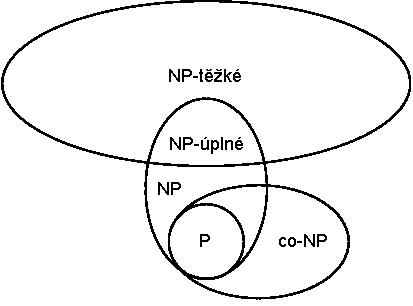
\includegraphics[scale=0.7]{img/complexity-classes.pdf}}
\caption{Schéma tříd složitosti}
\label{fig:complexity-classes}
\end{figure}

% uvést pojem metaheristika, heuristika
\section{Heuristické metody}
Heuristická metoda je postup, který umožňuje nalézt rozumně dobré řešení v relativně krátkém čase.
Metody jsou často iterativní, počínaje počátečním řešením, které se během každé iterace snaží vylepšit.
Po uplynutí přiměřeně dlouhé doby je ukončen a nejlepší řešení vráceno \cite{kaveh}.

Termín \textit{metaheuristika} byl zaveden v roce 1986 a skládá se ze dvou slov meta znamenající vyšší úroveň abstrakce a heuristiky znamenající umění objevovat pravidla k řešení problému.
Jsou to strategie, které využívají vyšší úroveň abstrakce spolu s heuristikou k prohledávání stavového prostoru s cílem nalezení nejlepšího řešení.
Jednou z jejich hlavních výhod je, že jsou nezávislé na daném problému.
Díky tomu nalezly uplatnění v různých oborech jako je lékařství, aplikovaná matematika, strojírenství nebo ekonomie \cite{kaveh, peres}.

Při prohledávání stavového prostoru je klíčové vyvážit fáze průzkumu (exploration) a vytěžování (exploitation).
Průzkum slouží jako prostředek pro \textit{diverzifikaci}, cílem je najít slibné oblasti s vysoce kvalitními řešeními.
Jakmile je oblast identifikována, přistoupí se k vytěžování, kdy je hledání v dané oblasti zintenzivněno \cite{peres}.

Metaheuristiky lze dělit do 2 kategorií na algoritmy založené na jediném řešení nebo na populaci.
Metaheuristiky založené na jednom řešení začínají s jedinou kandidátní konfigurací, kterou se snaží postupem času vylepšovat pomocí místního vyhledávání.
Nevýhodou těchto technik je, že mohou snadno uvíznout v lokálním optimu.
Patří mezi ně: tabu prohledávání, simulované ochlazování nebo řízené místní vyhledávání \cite{katoch}.

Na druhé straně metaheuristiky založené na populaci používají během vyhledávání více konfigurací.
Díky tomu je zachována diverzita, která ztěžuje uvíznutí v lokálním optimu.
Zahrnuje algoritmy, jako jsou: genetický algoritmus, optimalizace roje částic a optimalizace mravenčích kolonií \cite{katoch}.

\subsection{Simulované ochlazování}
Simulované ochlazovaní bylo vytvořeno v roce 1982.
Heuristika je založena na procesu žíhání pevné látky.
Účelem žíhání je donutit materiál se dostat do nízkoenergetického stavu, jako je krystal.
Proces spočívá v tom, že je materiál nejprve zahřán, což umožňuje vytvoření mnoha atomových přeskupení, a poté pomalu chlazen.
Na začátku existuje mnoho atomových uspořádání, ale postupem času při správném chlazení přetrvají jen ty dobré \cite{rutenbar}.

Algoritmus začíná s počáteční konfigurací a snaží se ji postupně vylepšit.
Aby nedošlo k uvíznutí v lokálním optimu, umožňuje přijmutí horší konfigurace.
V každé iteraci prohledává okolí aktuální konfigurace.
Každý krok je ohodnocen změnou energie $\Delta E$.
Je-li zlepšující $\Delta E\leq0$ nahradí aktuální konfiguraci, pokud je horší $\Delta E>0$ může být stále přijat.
Pravděpodobnost přijetí horší konfigurace je  vypočítána pomocí $p_a = e^{\frac{-\Delta E}{T}}$, kde $T>0$ je současná teplota.
Konfigurace je přijata, pokud platí $r<p_a$, kde $r$ je náhodné číslo z $ Unif(0, 1)$.
Pravděpodobnost přijetí horší konfigurace se s snižuje s $T$, nicméně je vždy nenulová \cite{rutenbar, kirkpatrik}.

Na konci každé iterace se aktuální teplota sníží.
Její průběh je řízen pomocí \textit{rozvrhu ochlazování}.
Klesání teploty je obecně nejrychlejší na začátku a ke konci se zpomaluje.
Zpočátku umožňuje diverzifikaci v podstatě náhodným prohledáváním konfiguračního prostoru.
Na závěr vede k intenzifikaci připomínající metodu iterativního zlepšování.
Na každé teplotě musí zůstat dostatečně dlouho, aby bylo dosaženo ustáleného stavu zvaném \textit{equilibrium} \cite{rutenbar, kirkpatrik}.

Algoritmus lze ukončit několika způsoby: dosažením maximálního počtu iterací, přestane se zlepšovat nebo dosáhne minimální teploty.
Pro použití heuristiky je třeba poskytnout celkem 4 komponenty: konfiguraci představující nastavení systému, náhodný generátor sousedních konfigurací, objektivní funkci a rozvrh ochlazování \cite{kirkpatrik}.

% \subsubsection{Vybrané rozvrhy ochlazování}

\subsection{Genetický algoritmus}
Genetický algoritmus je populační metaheuristika, která je inspirována přirozenou evolucí.
Napodobuje přežití nejzdatnějších jedinců.
Byla navržena v roce 1992.
Konfigurace jsou označovány jako jedinci.
Množina jednotlivců je nazývána populace.
Objektivní funkce se označuje jako fitness funkce a slouží k přiřazení zdatnosti jednotlivým jedincům.
Algoritmus používá 3 biologicky inspirované operátory: \textit{selekci}, \textit{křížení} a \textit{mutaci} \cite{katoch}.

Začíná s náhodně inicializovanou populací.
Nové generace jsou produkovány iterativně aplikací genetických operátorů.
Na začátku každé iterace jsou vybráni pomocí selekčního operátoru jedinci, kteří přežijí.
Vybraní jedinci jsou pak spárováni a kříženi.
Na výsledné potomky je s nějakou pravděpodobností aplikován operátor mutace.
Jako poslední dojde k nahrazení současné populace.
Proces se opakuje do splnění ukončovacího kritéria \cite{katoch}.

Kódování jednotlivců je závislé na problému, ale často se provádí pomocí binárního řetězce.
Hlavní výhodou je, že operátory křížení a mutace lze snadno a rychle implementovat 
Mezi další typy kódování patří permutační kódování, kódování hodnot a stromové kódování \cite{katoch}.

Selekce se používá k určení jedinců, kteří se budou účastnit reprodukce.
Je spojena s \textit{selekčním tlakem}, který umožňuje algoritmu konvergovat.
Určuje pravděpodobnost výběru zdatnějšího jedince.
Mezi známé algoritmy selekce patří: ruletový, turnajový nebo boltzmannův výběr \cite{katoch}.

Při použití ruletového výběru jsou nejprve jedinci z dané populace namapováni na kolo rulety.
Velikost výřezu je úměrná zdatnosti jedince.
Což znamená, že čím je daný jedinec zdatnější, tím větší je pravděpodobnost, že bude vybrán.
Při každém náhodném roztočení rulety je vybrán jeden jedinec.
Každý jedinec může být vybrán vícekrát \cite{katoch}.

Křížení se používá s cílem vytvořit nové potomky spojením genů dvou nebo více rodičů.
Existují dobře známé techniky jako jsou: jednobodové, vícebodové, cyklové a rovnoměrné křížení.
Dále může docházet k mutacím, které se vyskytují s určitou nízkou pravděpodobností.
Slouží k zavedení náhodných změn.
Simulují chyby, ke kterým dochází při kopírování chromozomů \cite{katoch}.

% popsat co je to mutace a křížení

\subsection{Tabu prohledávání}
Tabu prohledávání patří mezi metaheuristiky založených na jednom řešení.
K prohledávání stavového prostoru využívá adaptivní paměť, která umožňuje jeho efektivní prohledávání.
Prohledávacím prostorem se pohybuje aplikováním změn na aktuální konfiguraci.
Množina konfigurací dosažitelných z aktuální konfigurace se nazývá sousedství.
Operaci přesunu je používána k dosažení sousední konfigurace \cite{laguna}.

Algoritmus začíná hledat od počáteční konfigurace.
Během každé iterace je prohledáno sousedství současné konfigurace.
Nejprve je uplatněna strategie prvého zlepšení.
Pokud je nalezena lepší konfigurace, prohledávání sousedství je ukončeno a současná konfigurace nahrazena.
Pokud není nalezen žádný lepší tah, je současná konfigurace nahrazena nejlepším nezlepšujícím se sousedem.
Algoritmus je ukončen, jakmile je splněno ukončovací kritérium \cite{laguna}.

Dalším mechanismem, který pomáhá algoritmu překročit lokální optima, je \textit{krátkodobá paměť}.
Algoritmus si ukládá nedávnou historii tahů, které byly provedeny, a označuje je jako zakázané (tabu).
Tahy lze ukládat jako celé konfigurace.
Tento typ paměti se nazývá explicitní paměť.
Pokud jsou uloženy pouze vybrané atributy tahu, pak se paměť nazývá atributivní paměť.
Explicitní paměť obecně spotřebovává méně místa než atributivní paměť.
Pokud sousední konfigurace obsahuje nějaké tabu aktivní atributy, nelze ji přijmout jako současnou konfiguraci \cite{laguna}.

\textit{Tabu lhůta} (tenure) se používá k určení počtu iteracích, po které je daný atribut zakázaný.
Může být statická nebo dynamická.
K překonání tabu klasifikace lze použít \textit{aspirační kritérium}, které umožňuje při splnění určité podmínky přijmout zakázaného kandidáta.
Příkladem je nalezení lepší konfigurace, než je nejlepší dosud nalezená \cite{laguna}.

Pro řešení náročnějších problémů lze přidat \textit{dlouhodobou paměť}, která pomáhá lépe vyvážit proces diverzifikace a intenzifikace.
Paměť je obvykle založena na frekvenci změn jednotlivých atributů.
Pomáhá s lepším výběrem dalšího tahu \cite{laguna}.

\chapter{Algoritmické obchodování}
Algoritmické obchodování se používá k automatizaci obchodování pomocí počítačových programů.
Hlavním cílem je maximalizovat zisk a zároveň snížit rizika.
Vývoj těchto systémů vedl ke zrodu vysokofrekvenčního algoritmického obchodování, které drží pozice po extrémně krátkou dobu v řadech sekund až milisekund \cite{nuti, treleaven}.

Obchodování se uskutečňuje párováním nákupních a prodejních objednávek.
Párovací engine si vede centralizovanou knihu objednávek (order book).
Lze ji snadno vizualizovat jako tabulku se 2 sloupci, první s nákupními objednávkami a druhý s prodejními objednávkami.
Nákupní objednávky jsou řazeny sestupně, takže objednávka s nejvyšší cenou je první, jelikož cílem prodejce je prodat za co nejvyšší cenu.
Prodejní objednávky jsou seřazeny v obráceném pořadí, protože kupující chce koupit za nejnižší možnou cenu.
Po úspěšném spárování objednávek je provedena výměna (trade) \cite{nuti}.

Existují různé varianty knihy objednávek, které jsou závislé na dané burze.
Mohou podporovat plnění různých typů objednávek, jako jsou limitní, tržní (market) nebo objednávky se stop-lossem.
Tržní objednávky jsou provedeny okamžitě, zatímco limitní objednávky jsou splněny za stanovenou cenu nebo lepší.
Obchodování se provádí buď přímo přístupem na burzu, nebo prostřednictvím brokera, jako jsou banky.
Mezi aktiva, se kterými lze obchodovat, patří akcie, dluhopisy, opce, komodity, měnové páry, kryptoměny a deriváty \cite{nuti}.

Proces obchodování lze rozdělit do 4 fází: předobchodní analýza, generování obchodních signálů, provedení obchodu a poobchodní analýza.
Všechny lze automatizovat.
Během předobchodní analýzy je aktivum analyzováno na základě finančních dat a zpráv.
Výsledky se používají ke generování nákupních a prodejních signálů, které jsou následně převedeny na objednávky.
Proces lze formulovat jako optimalizační problém, který lze řešit pomocí kvadratického programování, genetického programování nebo optimalizace roje částic \cite{nuti}.

\section{Předobchodní analýza}
Předobchodní analýzu lze rozdělit do 3 kategorií: \textit{fundamentální}, \textit{technická} a \textit{kvantitativní} analýza.
Cílem fundamentální analýzy je určit férovou cenu aktiva.
Signály jsou obvykle generovány, když se aktuální cena aktiva liší od jeho férové ceny \cite{nuti}.

Technická analýza má za cíl předpovídat budoucí pohyb ceny aktiva na základě její \textbf{historie} a souvisejících informací, jako je objem.
Předpokládá, že všechny informace potřebné pro generovaní signálu se odrážejí v její historii.
Pracuje s konceptem trendů, které určují dlouhodobější směr pohybu ceny.
Trendy lze organizovat do vzorů, jako jsou trendové linie, oblasti podpory a odporu.
Používají se také technické indikátory jako klouzavé průměry, index relativní síly (RSI), stochastické oscilátory nebo pohyblivá průměrná konvergence/divergence (MACD).
Obchodní signály jsou generovány při změně trendu \cite{nuti}.

Kvantitativní analýza považuje ceny za náhodné a jejím cílem je vytvořit modely, které danou náhodnost dobře popisují.
Tím se liší od předchozích dvou typů analýz, které předpokládají deterministické chování ceny.
Stejně jako fundamentální analýza generuje obchodní signál, pokud se aktuální cena aktiva liší od jeho férové ceny \cite{nuti}.

\section{Generování obchodního signálu}
Výsledkem předobchodní analýzy jsou pouze doporučení k nákupu a prodeji, která jsou obohacena ve fázi generování obchodních signálu, kde jsou přidány informace, jako je cena a množství.
Skládá se ze vstupní a výstupní strategie.
Vstupní strategie určuje podmínky, kdy má program pozici otevřít, a výstupní strategie, kdy ji zavřít.
Rizika a velikosti objednávek musí být také řízeny \cite{nuti}.

Vstupní strategie mohou být jednoduché, jako je překřížení hodnot 2 technických indikátorů nebo odchýlení se od férové ceny.
I když je cílem pravidla co nejvíce zjednodušit, může být nutné přidat některá další pravidla.
Například otevírání obchodů může být příliš časté a na krátkou dobu, takže částka zaplacená na poplatcích převýší zisk.
Výstupní strategie definuje, kdy uzavřít zisk a kdy odejít se ztrátou.
Značně závisí na typu použité analýzy.
V případě technické analýzy může být pozice uzavřena, když je dosaženo určitého cíle nebo když se skutečný trend ukáže být odlišný od předpovídaného \cite{nuti}.

Řízení rizik se zabývá otázkou, jaká částka by měla být investována do každé objednávky.
Investovaná částka může být pevně stanovena pro každý obchod.
Nevýhodou této metody je, že nezohledňuje volatilitu trhu.
Může být méně riskantní investovat menší částky během období vysoké volatility a větší částky v obdobích nízké volatility.
Další metodou, kterou lze použít, je pevný zlomkový systém (fixed fractional system), který riskuje pevnou část kapitálu na každý obchod \cite{nuti}.

\section{Provedení obchodu}
Dalším krokem je samotné provedení objednávky.
Hlavní věc, které se systém snaží dosáhnout, je minimalizace nákladů.
V této fázi musí být rozhodnuto o typu objednávky a burze, na kterou má být objednávka zadána.
Mezi nejdůležitější aspekty, které je třeba vzít v úvahu při výběru správné burzy, patří: nabídka aktiv, mechanismus obchodování, cena provedení, likvidita a stupeň anonymity obchodníka.
Burzy s vyšší likviditou mají tendenci provádět objednávky rychleji a účtovat si nižší poplatky \cite{nuti}.

% Popsat PROM
\chapter{Zpětné testování}
Základní myšlenkou zpětného testování (backtesting) je zjistit, jak by fungovala obchodní strategie, kdyby byla nasazena v minulosti.
Vychází z předpokladu, že pokud strategie fungovala dobře v minulosti, měla by fungovat dobře i v budoucnu.
Zpětné testování je nezbytnou součástí rozvoje obchodní strategie, jelikož pomáhá lépe porozumět testované strategii a dává příležitost k jejímu zlepšení \cite{efficient-backtesting}.

Spuštění strategie na historických datech se nazývá historická simulace.
Během procesu se shromažďují různé statistiky, které jsou používány k vyhodnocení strategie.
Strategie jsou často parametrizované a nalezení jejich optimálních hodnot je NP-těžký problém.
Jednoduché metody jako hrubá síla nebo prioritní krokové vyhledávání jsou většinou nepoužitelné, protože nedokončí vyhledávání v dostatečně krátkém čase.
Proto se doporučuje používat sofistikovanější vyhledávací metody, jako je simulované ochlazování nebo genetický algoritmus
\cite{pardo, efficient-backtesting}.

Statistiky shromážděné během historické simulace se používají k formulaci optimalizačního kritéria.
Objektivní funkce založené na zisku jsou intuitivní volbou, ale ne nejlepší, protože mohou ignorovat podstatné nedostatky.
Upřednostňuje se použití pokročilejších kritérií, jako je CECPP a PROM, protože lépe odrážejí celkovou výkonnost strategie \cite{pardo}.

Dokonce i ta nejlepší nalezená konfigurace nemusí být nejlepší, protože může trpět jevem zvaným overfitting.
V zásadě to znamená, že strategie funguje velmi dobře na historických datech, na kterých byla optimalizována, ale podstatě hůře ve zkutečném obchodování \cite{pardo}.

% \cite{bowman}.
% overfitting
% need to be tested live
% paper trading
% representative data

% historická simulace by měla počítat s poplatky
\section{Historická simulace}
Nezbytnou součástí zpětného testování je historická simulace.
Slouží k vyhodnocení obchodní strategie na historických datech.
K provedení simulace musí být poskytnuta strategie a historická data.
Na základě obchodů provedených během simulace jsou vypočítány statistiky \cite{pardo}.

Výsledky jsou často prezentovány jako zpráva, která obvykle zahrnuje souhrn výkonnosti (performance summary) a výpis obchodů.
Souhrn výkonnosti se skládá ze statistik, které popisují celkovou výkonnost strategie.
Výpis obchodů obsahuje seznam všech uskutečněných obchodů s informacemi, jako je vstupní a výstupní čas, vstupní a výstupní cena a dosažený zisk nebo ztráta.
Mohou pomoci lépe porozumět tomu, jak se strategie chová během různých tržních období \cite{pardo}.

Simulace by měla být co nejpřesnější, jinak může vést k chybným závěrům a ztrátám při zkutečném obchodování.
Trhy používají různé zaokrouhlování svých cen, pokud simulátor používá nesprávně zaokrouhlené ceny, může to mít za následek neprovedení objednávek nebo nesprávné hodnoty zisku.
Chyby při zaokrouhlování mají obecně větší dopad na strategie, které obchodují častěji, protože rozdíl mezi otevírací a uzavírací cenou je menší \cite{pardo}.

Pokud jsou během simulace strategii poskytnuta data z většího časového rámce, jako jsou denní svíčky, tak může během daného období dojít k vytvoření více objednávek a jejich pořadí je nejednoznačné.
V reálném obchodování se cena, podle které se strategie rozhoduje, často aktualizuje, takže pořadí objednávek je dané.
Jedním ze způsobů, jak se zbavit nejednoznačnosti, je poskytnout strategii cenová data z nižšího časového rámce, jako jsou minutové svíčky.
Dalším používaným řešením je uhodnout pořadí objednávek \cite{pardo}.

Započítány by měly být i poplatky (commission) za vyřízení objednávky.
Bývají fixní a jejich velikost závisí na zprostředkovateli.
Dalším nákladem je cenový skluz (price slippage), ke kterému dochází při plnění objednávky.
Je to rozdíl mezi cenou objednávky (order price) a skutečnou cenou (fill price), za kterou bylo aktivum obchodováno.
Skluz je nízký, když je trh klidný a je málo objednávek, a vyšší, když je trh rušnější.
Záleží také na typu objednávky, velikosti objednávky a likviditě trhu \cite{pardo}.

\subsection{Výkonnostní statistiky}
Výkonnostní statistiky se používají k měření odměny a rizika.
Díky tomu, že jsou nezávislé na konkrétní obchodní strategii, tak poskytují způsob, jak je porovnat.
Statistiky lze nejen vypočítat na historických datech, ale lze je také použít pro měření výkonnosti běžící strategie v reálném čase.
Umožňují tedy kontrolu průběhu obchodování.
Zároveň jsou jediným způsobem, jak měřit a řídit riziko.
Mohou zahrnovat statistiky jako: celkový počet obchodů, počet vítězných a ztrátových obchodů, největší vítězný obchod, největší ztrátový obchod, celkový čistý zisk (total net profit), hrubý zisk (gross profit) a hrubá ztráta (gross loss) \cite{pardo}.

\begin{description}
    \item [realizovaný zisk (realized profit)] $rp$ je částka ztracená nebo získaná po uzavření pozice.
    Lze ji vypočítat pomocí vzorce $rp=tr-ti$, kde $tr$ je celkem získaná částka a $ti$ je celkem investovaná částka.
    Může být také vyjádřena v procentech $rp_p=\frac{rp}{ti}\cdot 100$.
    Pokud $rp\leq0$, tak se označuje jako ztráta, jinak jako zisk.
    \item[hrubý zisk (gross profit)] $gp\geq0$ je částka, která se spočítá jako součet realizovaných zisků všech ziskových uzavřených pozic $gp=\sum_{i=0}^{n} max(rp_i, 0)$, kde $n$ je počet uzavřených pozic.
    \item[hrubá ztráta (gross loss)] $gl\leq0$ je částka, která se spočítá jako součet realizovaných ztrát všech ztrátových uzavřených pozic $gl=\sum_{i=0}^{n} min(rp_i, 0)$, kde $n$ je počet uzavřených pozic.
    \item[celkový zisk (net profit)] $np$ lze vypočítat buď součtem realizovaných zisků všech uzavřených pozic $np=\sum_{i=0}^{n} rp_i$, kde $n$ je počet uzavřených pozic nebo $np=gp+gl$.
    \item [ziskový faktor (profit factor)] $pf$ lze spočítat $pf=\frac{gp}{|gl|}$.
    Pokud platí $pf>0$, tak byla strategie zisková, jelikož celkové zisky převyšují celkové ztráty.
    \item[zůstatek (balance)] $bn\geq0$ částka uložená na účtu.
    \item[současná hodnota] $cv$ je hodnota otevřené pozice, kdyby byla uzavřena za současnou tržní cenu $mp$.
    Lze ji vypočítat jako $cv=ps\cdot mp$, kde $ps$ je velikost pozice.
    \item[současný zisk] $cp$ je částka, která byla získána nebo ztracena za dobu po otevření pozice.
    Lze ji spočítat pomocí $cp=cv-ti$ nebo v procentech $cp_p = \frac{cp}{ti}\cdot 100$.
    \item[čistá hodnota (equity)] $eq\geq0$ je částka, která by byla na účtu, kdyby byla uzavřena aktivní pozice za aktuální cenu.
    Lze ji spočítat jako $eq=bn+cv$.
    \item[maximální sestupný pohyb (max drawdown)] $mdd\leq0$ je největší pozorovaná ztráta z vrcholu $p$ ke dnu $t$, do dosažení nového nejvyššího vrcholu.
    Lze ji vypočítat pomocí $mdd=t-p$ nebo v procentech $mdd_p=\frac{mdd}{p}\cdot 100$ \cite{max-drawdown}.
    \item[maximální vzestupný pohyb (max run-up)] $mru\geq0$ je největší pozorovatelný zisk ze dna $t$ k vrcholu $p$, do dosažení nového nejnižšího dna.
    Lze jej vypočítat pomocí $mru=p-t$ nebo v procentech $mru_p=\frac{mru}{t}\cdot 100$.
\end{description}

\section{Vizualizace}
Data získaná ze simulace lze dále vizualizovat pomocí grafu, což také pomáhá při ohodnocování a testování obchodní strategie.
Historická data jsou vykreslena pomocí svíčkového grafu, do kterého lze dále vykreslit hodnoty indikátorů, vstupní a výstupní body.
Čistá hodnota v každém okamžiku je často vykreslena na samostatném grafu pod svíčkovým grafem \cite{pardo}.

% doplnit o schéma
\subsection{Svíčkový graf}
Svíčkový graf umožňuje vizualizaci a analýzu historických dat.
Koncept vyvinul v 18. století japonský obchodník s rýží Munehisa Homma.
Na západě byly představeny mnohem později na konci 20. století Stevem Nisonem.
Graf může být použit k identifikaci vzorů a trendů \cite{candlestick-corporate}.

Skládá se ze svíček, které jsou grafickým znázorněním 4 klíčových cen: otevírací $o$, nejvyšší $h$, nejnižší $l$ a uzavírací $c$ ceny za daný časový interval.
Platí, že $l\leq h$.
Svíčka je tvořena 3 částmi: 2 knoty a tělem.
Knoty jsou znázorněny jako úsečky a tělo jako obdélník.
Horní knot začíná od středu horní strany těla a končí v úrovni $h$.
Spodní knot vede od středu spodní strany těla a končí na úrovni $l$.
Horní a spodní strana těla svíčky označují $o$ a $c$.
Pokud platí $o<c$, svíčka je rostoucí, jinak klesající.
Zároveň pokud je rostoucí, bývá tělo vybarveno zeleně, v opačném případě červeně \cite{candlestick-corporate}.

Svíčky jsou většinou dostupné ve formátu OHLC, což je zkratka pro otevírací (open), nejvyšší (high), nejnižší (low) a uzavírací (close) ceny.
Nejčastěji jsou ukládány do CSV souborů.
Používají se také pro historickou simulaci, pro kterou je třeba tyto čtyři hodnoty zredukovat na jedinou.
Obvykle se to provádí zprůměrováním cen a existuje několik běžně používaných metod: $hl2=\frac{h+l}{2}$, $hlc3=\frac{h+l+c}{3}$ nebo $ohlc4=\frac{o+h+l+c}{4}$.

\section{Historická tržní data}
Historická tržní data jsou nezbytnou součástí zpětného testování, jelikož bez nich nelze provést historickou simulaci.
Data je nutné pravidelně získávat a udržovat, často jen jejich získání v dostatečné kvalitě je obtížné \cite{pardo}.
Existují specializovaní poskytovatelé dat, jejichž cena se liší v závislosti na jejich kvalitě a množství.

Nejběžněji dostupná data jsou ve formátu OHLCV, což jsou OHLC a objem (volume) neboli množství obchodů uskutečněných v daném časovém intervalu.
Dále jsou ukládány samotné obchody ve formě obchodních tiků (trade ticks).
Pro dosažení větší přesnosti lze také použít nabídkové tiky (quote ticks), které ukládají údaje o nejlepší nabídce (bid) a poptávce (ask) z knihy objednávek v daném okamžiku \cite{polygon}.

% Doplnit o MultiChart
\section{Platformy poskytující zpětné testování}
V dnešní době existuje mnoho platforem nabízejících zpětné testování, liší se především druhem a množstvím dostupných historických dat, propracovaností, s jakou lze strategii implementovat, a částkou, kterou si účtují za používání jejich produktu \cite{bowman}.

\subsection{TradingView}
TradingView je oblíbená obchodní platforma, která umožňuje provádět technickou analýzu, vývoj a zpětné testování obchodní strategie.
Je přístupná jako webová, mobilní i desktopová aplikace. 
Nabízí širokou škálu tržních dat, jako jsou akcie, kryptoměny, indexy, energetické a zemědělské komodity, drahé kovy a Forex.
Základní funkce lze používat zdarma a pro přístup k pokročilejším jsou k dispozici různé cenové plány \cite{bowman}.

Používá se především pro vizualizaci dat a technickou analýzu, k čemuž nabízí nástroje pro kreslení do grafů a velké množství technických indikátorů.
Výsledné nápady lze uložit a sdílet s ostatními uživateli.
Grafy lze vizualizovat a organizovat různými způsoby \cite{tradingview}.

Strategie lze specifikovat pomocí programovacího jazyka PineScript a testovat pomocí zpětného testování, které je poměrně jednoduché.
Zpětné testování nabízí způsob nastavení strategie a vizualizace výsledků, které jsou k dispozici jako souhrn výkonnosti a seznam obchodů.
Neposkytuje způsob optimalizace parametrů \cite{tradingview}.

\section{Bazooka obchodní strategie}
Pro optimalizaci v praktické části práce byla vybrána obchodní strategie s názvem \textit{Bazooka}, která byla vytvořena a poskytnuta externím subjektem.
Jedná se o jednoduchou dobře definovanou a dříve otestovanou strategii, která pro rozhodování používá indikátory klouzavého průměru.
Využívá také mechanismus řízení rizik.
Strategie byla implementována na základě osobních setkání a ukázkové implementace v jazyku \textit{PineScript} pro platformu \textit{TradingView}.

K vyvolání otevíracího nebo uzavíracího signálu se používají klouzavé průměry, které mohou být typu EMA nebo SMA.
Obecně mohou být různé, například vstupní indikátor může být typu EMA s periodou 30 a výstupní indikátor může být typu SMA s periodou 20.
Indikátory jsou aktualizovány pomocí historických svíček v daném intervalu.
Pokud by byly například použity 30minutové svíčky, znamenalo by to, že by se indikátory aktualizovaly každých 30 minut s cenou získanou průměrem právě uzavřené 30minutové svíčky.

Strategie využívá více úrovní nákupu, které se získávají posunutím hodnoty vstupního ukazatele směrem dolů.
Hodnota každé úrovně $lv$ se získá pomocí $lv=env \cdot l$, kde $env$ je hodnota vstupního indikátoru a $l$ je zlomek určující posunutí.
Pro úrovně nákupu platí, že $\{l_0, l_1,\dots,l_n\} \in \mathbb{Q} \cap [0, 1] \land n>0 \land [\forall i \in \{0,\dots,n-1\} : l_i > l_{i+1}]$, kde $n$ je počet nákupních úrovní.
Nákupní signál je vyvolán, pokud nastane  $mp\leq lv_c$, kde $mp$ je současná nákupní cena a $lv_c$ je hodnota současné nákupní úrovně.
Nákup na každé úrovni lze provést pouze jednou.

Velikost nákupu $ps$ na každé úrovni je určena $ps=ibn \cdot s$, kde $ibn$ je počáteční zůstatek a $s$ je zlomek určující část, za kterou bude nákup proveden.
Pro velikosti nákupu platí, že $ (s_0, s_1,\dots,s_n) \in \mathbb{Q} \cap [0, 1] \land n>1 \land \sum_{i=0}^{n} s_i = 1 $, kde $n$ je počet nákupních úrovní.
Pokud například $(ibn=100 \land s = (\frac{2}{10}, \frac{5}{10}, \frac{3}{10}))\implies ps=(20, 50, 30)$.

Prodejní signál je vyvolán, pokud platí $mv\geq exv$, kde $exv$ je hodnota výstupního indikátoru a byla otevřena pozice.
Na rozdíl od vstupní strategie, která zvětšuje velikost pozice po částech, výstupní strategie prodává celou pozici najednou.
Strategie obchoduje, dokud není dosaženo minimálního vlastního kapitálu nebo je ručně vypnuta.

\section{Klouzavé průměry}
Klouzavé průměry jsou technické indikátory, jejichž cílem je určit trend daného aktiva výpočtem průměru jeho cen.
Existují 3 běžně používané indikátory: jednoduchý klouzavý průměr (SMA), exponenciální klouzavý průměr (EMA) a vážený klouzavý průměr (WMA).
Jsou počítány za určité období $k>0$, které určuje počet vzorků použitých k výpočtu.
Pokud je proveden SMA na cenách představujících 10 dní, nazývá se 10denní SMA.
Obvykle jsou vizualizovány společně s grafy cen akcií.
Křížení indikátorů lze použít k identifikaci změny trendu  \cite{ma-algorithms}.

\subsection{Jednoduchý klouzavý průměr}
Jednoduchý klouzavý průměr (SMA) je nejběžněji používaným ukazatelem klouzavého průměru a jak název napovídá, nejsnáze se počítá.
Průměrnou hodnotu posledních $k$ cen lze vypočítat pomocí $SMA_k = \frac{1}{k}\sum_{i=n-k+1}^{n} p_i$, kde $n$ je celkový počet cen a $p$ jsou samotné ceny.
Pro výpočet následující hodnoty lze využít $SMA_{k,next}=SMA_{k,prev}+\frac{1}{k}(p_{n+1}-p_{n-k+1})$, kde $p_{n+1}$ je nejnovější a $p_{n-k+1}$ nejstarší cena.
Lze jej efektivně implementovat pomocí datové struktury kruhový buffer.
Nejčastěji používané SMA jsou období 50, 100 a 200 dnů \cite{ma-algorithms, sma-wiki}.


\subsection{Exponenciální klouzavý průměr}
Na rozdíl od SMA, kde má každá hodnota při výpočtu průměru stejnou váhu, tak exponenciální klouzavý průměr (EMA) přiřazuje cenám váhy.
Hodnoty vah klesají exponenciálně, takže novější hodnoty mají větší váhu a tím i větší vliv na výslednou průměrnou hodnotu.
Díky tomu reaguje rychleji na změny ceny aktiva než SMA.
Obvykle se používá k výpočtu průměru za kratší časové období \cite{ma-algorithms, ema-institute}.

Počáteční hodnota se vypočítá pomocí SMA se stejnou periodou.
Následující hodnoty lze získat použitím
$EMA_{k, next} = p_c \cdot wf + EMA_{k, prev} \cdot (1-wf) \land wf=\frac{sf}{k+1} \land sf\geq2$, kde $p_c$ je současná cena, $wf$ je vážený faktor a $sf$ je vyhlazovací faktor.
Vážený faktor se používá k určení množství váhy, která je přiřazena nejnovější hodnotě.
Například pokud $k=10 \land sf=2 \implies wf = 0,1818$, což znamená, že 18,18 \% celkové hmotnosti je přiřazeno nejnovější hodnotě \cite{ma-stockcharts}.

\chapter{Volba technologie}
\section{Programovací jazyky}
Pro hlavní část aplikace, kde byla požadována rychlost, bylo použito C++ a pro účely vizualizace výsledků Python.
Oba jazyky nabízejí vysokou úroveň abstrakce, ale liší se v prioritách.
Python je jednoduchý jazyk, který umožňuje soustředit se více na řešení problému než na správu počítačových prostředků.
C++ se naproti tomu zaměřuje na efektivitu za cenu vyšší komplexnosti.

\subsection{C++}
C++ je programovací jazyk na vysoké úrovni vyvinutý v roce 1983 \textit{Bjarnem Stroustrupem} v Bell Labs jako rozšíření programovacího jazyka \textit{C}.
Jedná se o multiparadigmatický programovací jazyk, který podporuje datovou abstrakci, objektově orientované programování, procedurální programování a generické programování \cite{cpp}.

V programátorské komunitě je dobře známý a hojně používaný například pro vývoj herních enginů, prohlížečů, aplikací a provádění vysoce-výkonných výpočtů (HPC).
Na základě indexu TIOBE za březen 2023 byl ohodnocen jako číslo 4 v popularitě, velmi těsně za programovacím jazykem Java.
Byl také vyhodnocen jako programovací jazyk roku 2022 stejnou společností díky jeho rostoucí popularitě  \cite{tiobe}.

Mezi verzemi C++03 a C++11 byla obrovská mezera, což mohl být důvod, proč mnoho lidí od jazyka raději ustoupilo.
Od C++11 se však každé 3 roky objevují nové verze jazyka, které do jazyka zavedly nové funkce, zlepšily bezpečnost práce s pamětí a pomohly mu získat větší důvěru.
Posledním vydaným standardem je C++20 a nejnovější standard se chystá být vydán letos.

Je to bohatý jazyk s rozsáhlou standardní knihovnou.
Ve srovnání s jinými modernějšími jazyky, jako je Python, je však obtížnější se naučit a správně používat.
Jazyk je staticky typován, což znamená, že typ objektu musí být při deklaraci explicitně specifikován.
Na rozdíl od Pythonu, který je interpretován za běhu, je C++ kód kompilován.
Ve srovnání s Pythonem trvá psaní kódu obecně více času, protože programátor musí být konkrétnější, což může určitou skupinu programátorů odradit.
Má ale jednu věc, kterou Python postrádá, a tou je rychlost.

C++ nabízí generické programování, k čemuž jsou používány šablony.
Existují pouze během kompilace.
Umožňují použití statického polymorfismu, který za běhu stojí méně prostředků než známější dynamický polymorfismus využívající virtuální funkce.
V nejnovějších standardech byly zavedeny některé funkce, které se vyhýbají použití dynamického polymorfismu, jako například: \texttt{std::optional} a \texttt{std::variant}.

Další věcí, kterou nabízí ke zrychlení kódu, jsou optimalizace, které lze nastavit během kompilace.
Pracují s konceptem pozorovatelného chování, které umožňuje produkci jiného byte kódu, který dělá stejnou věc rychleji.
Využívá proto datovou a funkční nezávislost.

Paralelní zpracování lze také použít ke zrychlení kódu.
Program může být spuštěn na jiném procesu nebo různých vláknech nebo obojí.
Standardní knihovna nabízí implementaci vláken a souvisejících nástrojů, lze však použít i OpenMP framework.
Zpracování na více procesech najednou lze zajistit například použitím MPI frameworku.
Ne všechny programy jsou vhodné pro paralizaci, ale je dobré, že je tu možnost ji použít.
Například v Pythonu existuje koncept vláken, nicméně v jednom procesu může současně běžet pouze jedno vlákno díky Global Interpreter Lock (GIL).

Kromě standardní knihovny je k dispozici mnoho open-source, dobře navržených a testovaných knihoven.
Existují knihovny Boost, které nabízejí knihovny pro síťování (Asio), unit testování (Test), paralelní zpracování (MPI) a mnoho dalších, jako je POCO, JSON pro moderní C++, Google Test a OpenCV.

\subsection{Python}
Programování v Pythonu je dynamicky typovaný, interpretovaný programovací jazyk, který vytvořil Guido van Rossum v roce 1991.
Podporuje objektově orientované i funkční programování.
Je vyvinut a spravován Python Software Foundation.
Nejnovější verze jazyka je 3.11 \cite{python}.

Ve srovnání s C++ je mnohem snazší se jej naučit.
Vyznačuje se jasnou a čitelnou syntaxí.
Má rozsáhlou standardní knihovnu a 2 správce balíčků Pip a Conda.
V březnu 2023 se umístil na 1. místě v oblíbenosti podle indexu TIOBE.
Používá se hlavně pro vývoj webových aplikací, skriptování a strojové učení.

V posledních letech je to dominantní jazyk používaný ve strojovém učení díky frameworkům jako jsou: TensorFlow, PyTorch a scikit-learn.
Existují také balíčky datové vědy, jako jsou: NumPy, SciPy, Pandas a Matplotlib.
Všechny je lze použít v Jupyter Notebook, což je interaktivní webová výpočetní platforma, která usnadňuje zpracování a vizualizaci dat.

Hlavní nevýhodou jazyka je, že ve srovnání s jazyky jako C++ je pomalý.
Existují balíčky, jako je NumPy, které jsou napsány částečně v C programovacím jazyku, nebo dokonce vysoce výkonné kompilátory, jako je Numba, které lze použít k urychlení kódu.
Obecně je však z hlediska výkonu lepší použít jiný jazyk.
Co však Python ztrácí na výkonu, to vynahradí vysokou flexibilitou, rozsáhlou komunitou programátorů a velkým množstvím užitečných balíčků.

\chapter{Design}

\section{Jmenné konvence}
Konvence pojmenování jsou převzaty převážně z \textit{STL} a \textit{Boost} knihoven.
Názvy tříd a funkcí používají \texttt{snake\_case}.
Metody nastavení a čtení atributů třídy nepoužívají \texttt{set} a \texttt{get} ve svém názvu, jsou jednoduše odlišeni tak, že gettery neberou žádný parametr a settery berou více než jeden.
Názvy šablon a konceptů používají \texttt{CamelCase}.
Soukromé atributy třídy končí podtržítkem.

\section{Uspořádání projektu}
Projekt je rozdělen do 3 hlavních adresářů: \textit{include}, \textit{src} a \textit{test}.
Adresář \textit{include} obsahuje obchodovací framework a vybrané hlavičkové soubory z knihovny CppCoro.
Organizace frameworku je inspirovaná knihovnou \textit{Boost.Asio}.
Definice a deklarace tříd jsou uloženy společně v jednom souboru s příponou \textit{.hpp}.
Hierarchie složek se řídí jmennými prostory, například třídu \texttt{trading::bazooka::long\_strategy} lze nalézt v souboru \textit{/include/trading/bazooka/long\_strategy}.
Framework lze zahrnout jako celek pomocí \textit{trading.hpp} nebo jednotlivě po souborech.

Adresář \textit{src} se skládá ze souboru \textit{main.cpp}, Jypiter Notebooků používaných pro vizualizaci, vstupních a výstupních dat.
Testy jsou organizovány stejně jako třídy obchodovacího frameworku.
Projekt je kompilován pomocí souborů \textit{CMakeLists.txt}, které obsahují seznam souborů ke kompilaci, nastavení kompilátoru a informace pro hledání externích knihoven.
Vytváří 2 spustitelné soubory \textit{backesting} pro použití optimalizátorů a \textit{test\_} pro provádění testů.

\section{Návrhové vzory}
Účelem návrhových vzorů je snížit složitost kódu a šanci udělat chybu.
Existuje celá řada známých a dobře popsaných návrhových vzorů, je však nutné rozpoznat situace, kdy je vhodné je použít.
Obecně slouží jako řešení běžně se vyskytujících problémů, nelze je však importovat z knihovny.
Je to jen koncept s nějakou základní myšlenkou, kterou lze aplikovat různým způsobem v závislosti na konkrétním problému.
V následujících částech jsou popsány pouze ty, které byly použity v samotném projektu \cite{design-pattern}.

\subsection{Pozorovatel}
Návrhový vzor pozorovatel (observer) umožňuje objektům nazývaným pozorovatelé být upozorňováni na události, které nastanou u pozorovaného objektu.
Pozorovatelé se přihlásí k odběru oznámení o událostech, které nastávají u pozorovaného objektu, a jsou upozorněni, kdykoli k nim dojde \cite{observer}.

Pozorovaný objekt musí být nejprve předán pozorovanému objektu, obvykle pomocí vyhrazené metody.
Poté, kdykoli dojde k události, je zavolána specifická metoda pozorovatele s událostí spojená.
Tím se pozorovatel a pozorovaný stávají na sobě nezávislými, pozorovatel musí pouze splňovat dohodnuté rozhraní \cite{observer}.

Vzor pozorovatel se používá pro upozornění na události, které nastanou během optimalizačního procesu a simulace obchodování.
Informace shromážděné během simulace lze použít k výpočtu výkonnostních statistik nebo ke sběru dat pro vizualizaci.
Pozorovatelé jsou dodáváni při volání instance třídy a jsou předávány jako sada šablonových parametrů.
Což umožňuje předání žádného, jednoho nebo více pozorovatelů, kteří mohou být různého typu, avšak musí být známy v době kompilace.

\subsection{Strategie}
Účelem strategického vzoru (strategy) je zapouzdřit rodinu podobných algoritmů se stejným účelem do samostatných tříd a učinit je vzájemně zaměnitelnými.
Třídy těchto algoritmů se nazývají strategie \cite{strategy}.

Třída používající strategii se většinou nazývá kontext.
Neví nic o strategii, která je ji předána.
Jediné, co musí strategie splňovat, je dohodnuté rozhraní.
Díky tomu je kontext nezávislý na konkrétní strategii.
Volba vhodné strategie je na uživateli aplikace.
Algoritmy obvykle implementují jednu společnou metodu, která musí přebírat setjnou sadu argumentů.
Voláním této metody se spustí daný algoritmus \cite{strategy}.

V práci je vzor strategie použit pro výběr různých druhů rozvrhů chlazení pro algoritmus simulovaného ochlazování.
Strategie je předána instanci optimalizátoru jako parametr při jeho volání.
Musí splňovat koncept \texttt{simulated\_annealing::Cooler}.
Jelikož různé algoritmy chlazení vyžadují různé sady argumentů, je při volání strategie předána přímo instance optimalizátoru.
Volba požadovaného parametru jako je aktuální teplota nebo počet proběhlých iterací je na strategii samotné.
Je navržen hlavně pro použití pro statický polymorfismus, ale lze mezi strategiemi přepínat za běhu pomocí \texttt{std::function}, který používá \textit{type erasure}.

\chapter{Simulace obchodování}
Simulace obchodování byla inspirována kryptoměnovou burzou \textit{Binance}.
Byly přijaty některé konvence pojmenování, jako je otevírání a zavírání pozic.
Otevření longové pozice znamená nákup aktiva, nicméně otevření shortové pozice znamená jeho prodej.
Prodej a nákup tedy jdou proti sobě, a proto je lepší používat termíny otevření a uzavření.

Je také běžné zaměnitelně říkat, že obchod nebo pozice jsou otevřené.
Na \textit{Binance} je možné si vyžádat historii uskutečněných obchodů.
Vygenerované obchody jsou pouze transakce provedené mezi dvěma obchodníky.
Proto je lepší používat termín pozice, který představuje seznam souvisejících otevřených a uzavřených obchodů.
% popsat jak funguje Binance
% Účet je na kryptoburzách reprezentován jako peněženka, která uchovává množství nakoupených aktiv.

\section{Bazooka}
Strategie s názvem \textit{Bazooka} byla rozdělena do 2 tříd: \texttt{bazooka::strategy} a \texttt{bazooka::manager}.
Důvodem rozdělení bylo oddělení zájmů.
Třída \texttt{bazooka::strategy} dělá rozhodnutí a třída \texttt{bazooka::manager} je realizuje.
V současné době je implementována burza podporující pouze longové obchody, ale pokud by v budoucnu existovala např. \texttt{futures::market} burza podporující pákové obchody, bylo by nutné použít jiný typ manažera, nicméně strategie by zůstala stejná.
Jsou dány dohromady pomocí třídy \texttt{trader}.

Hodnoty nákupních velikostí a úrovní jsou uloženy jako pole zlomků pevné délky.
Zlomky jsou reperezentovány pomocí třídy \texttt{fraction}, která je inspirována třídou \texttt{boost::rational}.
Je však mnohem jednodušší a méně obecná.
Předpokládá, na rozdíl od \texttt{boost::rational}, že zlomky, mezi kterými se provádějí aritmetické operace, mají stejného jmenovatele.
Porušení tohoto předpokladu vede k nedefinovanému chování.
Zlomky jsou uloženy v instanci třídy \texttt{std::array}, což také znamená, že velikost sekvence musí být známa v době kompilace.

\subsection{Strategie}
% dát pryč nebo přidat long/short strategy
Strategie je implementována pomocí třídy \texttt{bazooka::strategy}.
Má jeden parametr šablony třídy \texttt{n\_levels}, který uvádí počet úrovní nákupu.
Při inicializaci přebírá parametry: vstupní a výstupní indikátor a úrovně nákupu.
V průběhu inicializace jsou také validovány nákupní úrovně, pokud nesplňují požadavky, je vyhozena výjimka \texttt{std::invalid\_argument}.

Účelem třídy je činit rozhodnutí a k tomu má dvě metody \texttt{should\_open} a \texttt{should\_close}.
Obě metody používají indikátory, aby zjistily, zda byly splněny podmínky pro vyslání signálu.
Vracejí booleovskou hodnotu, která určuje, jestli by měla být akce provedena.
V jednu chvíli může nastat pouze jedna událost.
Indikátory jsou aktualizovány pomocí metody \texttt{update\_indicators}.
Vstupní a výstupní hodnoty lze získat voláním getrů třídy.
Lze je použít pro vykreslování grafů.

\subsection{Indikátor}
Indikátor může být typu \texttt{sma} nebo \texttt{ema}.
Běžným způsobem, jak umožnit oba typy, by bylo použití runtime polymorfismu prostřednictvím virtuálních funkcí.
Oba indikátory by musely dědit ze společné třídy a implementovat její virtuální funkce.
Instance třídy by musela být inicializována na haldě namísto zásobníku a dalo by se k ní přistupovat pomocí ukazatele na společnou třídu.
Jak dynamická alokace, tak použití virtuálních funkcí způsobují režii navíc.
Existuje několik nedávných přednášek z \textit{C++ konference} (CppCon) \cite{gobel-virtual, bogosavljevic-virtual}, které jsou zaměřeny na způsoby, jak se vyhnout používání virtuálních funkcí.
V obou přednáškách jsou zapojeny prvky moderního C++.

Jako nejvhodnější se v tomto případě nabízí použití třídy \texttt{std::variant} zavedené standardem C++17.
Třída funguje jako uložiště pro různé typy.
Pro uložení instance daného typu používá staticky alokované pole bajtů, který má velikost největšího uložitelného typu.
Jako třídní šablonové parametry přebírá seznam typů, které mohou být v objektu uloženy.
K hodnotě uložené v instanci objektu lze přistupovat pomocí funkce \texttt{std::get}.
Funkce přijímá šablonový argument, který je buď indexem typu, nebo samotným typem, který by měl být aktuálně v instanci uložen.
Pokud je uložen jiný typ, tak volání funkce způsobí vyhození \texttt{std::bad\_variant\_access} výjimky.

Dalším způsobem přístupu k uložené hodnotě je použití funkce \texttt{std::visit}.
Vyžaduje 2 argumenty, první je volatelný objekt a druhý instance třídy \texttt{std::variant}.
Funkce při volání nejprve získá hodnotu uloženou v instanci a poté ji předá volatelnému objektu.
V případě indikátorů může být použita například při jeho aktualizaci (viz \ref{lst:update:indicator}).

\begin{lstlisting}[caption={~Aktualizace indikátoru pomocí std::visit},label={lst:update:indicator},captionpos=t,abovecaptionskip=-\medskipamount,belowcaptionskip=\medskipamount,language=C]
std::variant<sma, ema> ma{sma{30}};
bool ready = std::visit([&value](auto& indic) {
    return indic.update(value);
}, ma);
\end{lstlisting}

Aby bylo možné objekt zapouzdřit a snadněji spravovat, byla vytvořena třída \texttt{bazooka::indicator}.
Třída má pouze jeden členský atribut \texttt{data\_} typu \texttt{std::variant<sma, ema>}, který je používán pro uložení indikátoru.
Metody používají \texttt{std::visit} pro přístup a změnu hodnoty indikátoru.
Sdílí stejné rozhraní s třídami \texttt{sma} a \texttt{ema}.

\subsubsection{Indikátory založené na klouzavém průměru}
Byly implementovány dva indikátory založené na klouzavém průměru \texttt{sma} a \texttt{ema}.
Sdílejí stejné rozhraní.
Jsou aktualizovány voláním metody \texttt{update} a jejich hodnotu lze získat voláním metody \texttt{value}.
Metoda \texttt{update} vrací hodnotu boolean indikující, zda je indikátor připraven.
Lze to také zkontrolovat voláním metody \texttt{is\_ready}.

Počáteční hodnota indikátoru \texttt{ema} je získána pomocí indikátoru \texttt{sma} se stejnou periodou.
Další hodnoty se vypočítají pomocí vzorce, který používá aktuální hodnotu.
Třída \texttt{sma} používá \texttt{boost::circular\_buffer} k uložení předchozích hodnot pro výpočet průměru.
Jakmile je buffer plný, tak je indikátor připraven.

\subsection{Manažer}
Účelem manažera je realizovat akce vytvořené strategií.
Je implementován pomocí třídy \texttt{bazooka::manager}.
Komunikuje s burzou a zabývá se tvorbou objednávek a řízením rizik.
Dvě nejdůležitější metody pro vytváření objednávek jsou \texttt{create\_open\_order} a \texttt{create\_close\_all\_order}.
Objednávky jsou reprezentovány strukturou \texttt{order}, která obsahuje 3 atributy: prodané množství, cenu, za kterou bylo aktivum nakoupeno/prodáno, a čas jejího vytvoření.

Strategie používá $n$ nákupních úrovní.
Vždy začíná obchodovat s počátečním zůstatkem, který je rozdělen na $n$ velikostí nákupu.
Skutečné velikosti objednávek lze vypočítat buď na začátku, nebo průběžně.
Výpočet velikostí objednávek za běhu se zdálo být přirozenější, takže byla implementována třída \texttt{order\_sizer}.
Při konstrukci přijímá pole velikostí objednávek $s$ a převádí jej na pole akumulovaných velikostí $a$, kde platí, že $s_0 = a_0 \land a_n = 1 \land [\forall i \in \{0,\dots,n\} : a_i = \sum_{j=0}^{i} s_j]$.
Po zavolání instance je vynásoben zůstatek aktuální akumulovanou velikostí pro získání velikosti objednávky.

Vzhledem k tomu, že má manažer přístup k burze, tak poskytuje metody pro přístup k jejímu aktuálnímu stavu, jako je zůstatek peněženky, čistá hodnotu a aktuální zisk aktivní pozice.
Jakmile je objednávka provedena, je uložena jako poslední otevřená/uzavřená objednávka a lze k ni přistupovat prostřednictvím getrů třídy.
Je to cenná informace pro vykreslování grafů a výpočet statistik.
Může nebo nemusí být použita, takže je lepší ji uložit samostatně a neustále ji přepisovat, než všechny ukládat například do instance \texttt{std::vector}, což by způsobilo zbytečnou režii navíc.

\section{Obchodník}
Funkcionality tříd \texttt{bazooka::manager} a \texttt{bazooka::strategy} jsou propojeny pomocí \texttt{bazooka::trader}.
Pro zpřístupnění veřejných metod obou tříd je použita vícenásobní veřejná dědičnost.
Třída poskytuje metodu \texttt{trade} \ref{lst:trade}, která používá metody obou tříd.
Strategie činí rozhodnutí, která manažer uskutečňuje.
Metoda vrací výčet \texttt{action} udávající, která akce byla provedena.

\begin{lstlisting}[caption={~Implementace metody trade třídy \texttt{bazooka::trader}},label={lst:trade},captionpos=t,abovecaptionskip=-\medskipamount,belowcaptionskip=\medskipamount,language=C]
action trade(const price_point& curr)
{
    action done{action::none};
    if (!Strategy::is_ready()) return done;

    if (Strategy::should_open(curr.data)) {
        Manager::create_open_order(curr);
        done = action::opened;
    }
    else if (Strategy::should_close_all(curr.data)) {
        Manager::create_close_all_order(curr);
        done = action::closed_all;
    }
    return done;
}
\end{lstlisting}

\section{Burza}
Burza je implementována pomocí třídy \texttt{market}.
Ve srovnání se skutečnou burzou je to velmi zjednodušená.
Podporuje pouze objednávky typu long a jeden uživatelský účet.
Mezi třídní atributy patří: aktivní pozice, poslední uzavřená pozice, peněženka a výše poplatků spojených s realizací objednávek.

Peněženka je implementována třídou \texttt{wallet} a slouží ke správě zůstatku zákaznického účtu.
Zůstatek lze snížit voláním metody \texttt{withdraw} nebo navýšit použitím \texttt{deposit}.
Pokud je částka k výběru větší než aktuální zůstatek, tak je vyhozena výjimka \texttt{insufficient\_funds}.
Aktivní pozice je uložena v instanci \texttt{std::optional}, jelikož pozice nemusí být otevřena.

Pomocí metody \texttt{fill\_open\_order} může být aktivní pozice otevřena nebo navýšena v závislosti na tom, zda již existuje.
Po otevření lze pozici uzavřít jako celek pomocí \texttt{fill\_close\_all\_order} metody, nikoli po částech.
Třída také poskytuje getry pro získání přístupu k aktuální čísté hodnotě, kontrolu, zda je otevřená pozice, nebo zjištění aktuálního zisku aktivní pozice.

\section{Pozice}
Pozice je implementována třídou \texttt{position}.
Lze ji otevřít vytvořením instance třídy, zvýšit voláním metody \texttt{increase} nebo uzavřít pomocí metody \texttt{close}.
Celkové množství nakoupeného aktiva lze zjistit voláním metody \texttt{size}.
Dále lze získat aktuální hodnotu a aktuální zisk.
Vzhledem k tomu, že je v průběhu ukládán celkový realizovaný zisk a celková investovaná částka, tak je lze zjistit i po uzavření pozice.
Při změně velikosti pozice jsou uplatňovány poplatky.
Výše otevíracích a uzavíracích poplatků jsou poskytnuty při inicializaci.

\section{Simulátor}
Obchodování lze simulovat pomocí třídy \texttt{simulator}, která uchovává a připravuje historická data pro simulaci a umožňuje její provedení.
Hlavním účelem třídy je použít ji jako objektivní funkci během optimalizace.
Obchodování lze pozorovat pomocí pozorovatelů.
Tímto způsobem lze například použít třídu \texttt{bazooka::statistics::collector} ke sběru statistik nebo ke sběru časových řad třídu \texttt{chart\_series::collector}, které mouhou být použity pro vykreslování grafů.

Při inicializaci jsou předány simulátoru historické ceny v podobě minutových svíček.
Pro rozhodování se používají minutové uzavírací ceny.
Ceny používané pro aktualizaci indikátorů jsou získány tak, že jsou minutové svíčky nejprve převzorkovány pomocí \texttt{resampler} na požadované časové období a zprůměrovány pomocí zvolené průměrovací metody.
Pokud je například doba převzorkování 30 minut a metoda průměrování \textit{OHLC4}, tak jsou svíčky nejprve převzorkovány na 30minutové svíčky a poté zprůměrovány pomocí \texttt{candle::ohlc4}.

Proces převzorkování probíhá tak, že za dané období se otevírací cena první svíčky stane otevírací cenou převzorkované svíčky a uzavírací cena poslední svíčky se stane její uzavírací cenou.
Vysoká a nízká cena jsou nejvyšší a nejnižší ceny v daném období.
Jelikož je převzorkování poměrně časově náročné, tak se provádí pouze jednou v konstruktoru, takže se neopakuje při každém volání simulátoru.

Simulátor při volání přebírá instanci obchodníka a seznam pozorovatelů \ref{lst:simulator}.
Iteruje přes rozhodovací ceny až do konce nebo dosažení minimální čisté hodnoty.
Pozorovatelé jsou během optimalizace informováni o událostech, jako je otevření pozice nebo aktualizace indikátoru.
Ceny použité pro aktualizaci indikátoru jsou procházeny pomocí iterátoru.

\begin{lstlisting}[caption={~Implementace simulace obchodování},label={lst:simulator},captionpos=t,abovecaptionskip=-\medskipamount,belowcaptionskip=\medskipamount,language=C]
template<class Trader, class... Observer>
void operator()(Trader&& trader, Observer& ... observers)
{
    auto indic_prices_it = indic_prices_.begin();

    (observers.begin(trader, prices_.front()), ...);
    for (std::size_t i{0}; i<prices_.size() &&
        trader.equity(prices_[i].data)>min_equity_; i++) {
        (observers.traded(trader,trader(prices_[i]),prices_[i]),...);

        if (trader.has_active_position())
            (observers.position_active(trader, prices_[i]), ...);

        // update indicators
        if (i && (i+1)%resampling_period_==0)
            if (trader.update_indicators((*indic_prices_it++)))
                (observers.indicators_updated(trader, prices_[i]), ...);
    }
    (observers.end(trader, prices_.back()), ...);
}
\end{lstlisting}

\section{Statistiky}
Nezbytnou součástí optimalizace jsou statistiky, jelikož jsou použity k formulaci optimalizačního kritéria a omezujících podmínek.
Statistiky, které jsou společné pro všechny obchodní strategie, jsou reprezentovány třídou \texttt{statistics} a jsou rozšířeny pro \textit{Bazooka} obchodovací strategii \texttt{bazooka::statistics}.

Instance třídy je inicializována předáním počátečního zůstatku.
Statistiky jsou aktualizovány pomocí metod pro aktualizaci \texttt{update\_equity()} nebo setrů \texttt{set\_final\_balance}.
K uloženým statistikám lze přistovat pomocí getrů.
Některé hodnoty, jako je celkový zisk, lze získat buď jako částku nebo v procentech.
Pro upřesnění jednotky a se používá značka \texttt{percent} nebo \texttt{amount} \ref{lst:use:unit:tag} při volání metody.

\begin{lstlisting}[caption={~Metody pro získání celkového zisku v různých jednotkách},label={lst:use:unit:tag},captionpos=t,abovecaptionskip=-\medskipamount,belowcaptionskip=\medskipamount,language=C]
template<class T>
requires std::same_as<T, amount>
amount_t total_profit() const
{
    return final_balance_-init_balance_;
}

template<class T>
requires std::same_as<T, percent>
percent_t total_profit() const
{
    return ((final_balance_-init_balance_)/init_balance_)*100;
}
\end{lstlisting}

Všechny statistiky související se ziskem jsou sledovány pomocí instance \texttt{profit\_statistics}, které lze použít k získání hrubého zisku, hrubé ztráty nebo faktoru zisku.
Dále jsou sledovány statistiky související s pohybem pomocí \texttt{motion\_statistics}, které poskytují minimální a maximální hodnotu, maximální vzestupný a sestupný pohyb.
Vzestupný pohyb je sledován pomocí \texttt{run\_up\_tracker} a sestupný pomocí \texttt{drawdown\_tracker}.
Tím to způsobem jsou sledovány čistá hodnota a uzavírací zůstatek.
Hodnoty lze opět vyjádřit v procentech nebo částkách.

Do třídy \texttt{bazooka::statistics} byl přidán čítač otevíracích objednávek pro jednotlivé nákupní úrovně.
Nese informace o tom, kolikrát bylo dosaženo jednotlivých úrovní nákupu, a může tak pomoci lépe porozumět tomu, jak se strategie chová.

\chapter{Další}
\section{Čtení a zápis do souborů}
Byly vytvořeny vlastní třídy pro čtení a zápis do souborů \textit{CSV}.
Jsou užitečné při čtení historických svíčkových dat a při ukládání časových řad pro vykreslování grafů.
Pro uložení nastavení a výsledků experimentu byl zvolen formát \textit{JSON} (\textit{JavaScript Object Notation}), který je standardizovaný a čitelný.
V tomto případě nebylo nutné vytvářet vlastní implementaci, protože existuje dobře známá, používaná a udržovaná knihovna \texttt{nlohmann/json} \cite{lohmann}.

% popsat JSON a vlatsní třídy

\subsection{Formát CSV}
Pro čtení a zápis do souborů \textit{CSV} (\textit{Comma-Separated Values}) byly vytvořeny třídy \texttt{csv::reader} a \texttt{csv::writer}.
Hodnoty jsou uloženy v tabulce, kde sloupce jsou hodnoty stejného typu odděleny oddělovačem, obvykle čárkou.
První řádek může obsahovat názvy sloupců, ale nemusí.

Obě třídy mají jeden třídní šablonový udávající počet sloupců.
Při inicializaci přebírají jako parametr cestu k souboru uloženému v instanci \texttt{std::filesystem::path} a oddělovač.
Soubor je otevřen při konstrukci třídy, pokud jej nelze otevřít, je vyhozena výjimka \texttt{std::runtime\_error}.
Soubor je uzavřen při destrukci objektu.

Třída \texttt{csv::reader} nabízí dvě metody pro čtení řádků: \texttt{read\_header} a \texttt{read\_row}.
Je přirozenější číst názvy sloupců do instance \texttt{std::array} než přímo do proměnných.
Čtení přímo do proměnných je dosaženo použitím sady šablonových parametrů \ref{lst:csv:read:row}.
Třída vrací booleovský příznak s informací o tom, zda byl řádek přečten nebo ne.
Hodnoty pak lze snadno číst v cyklu \texttt{while} (viz \ref{lst:read:candles}).
Třída \texttt{io::parser} je používána k parsování jednotlivých hodnot.

\begin{lstlisting}[caption={~Implementace čtení řádky třídy \texttt{io::csv::reader}},label={lst:csv:read:row},captionpos=t,abovecaptionskip=-\medskipamount,belowcaptionskip=\medskipamount,language=C]
template<class ...Types>
bool read_row(Types& ...inputs)
{
    static_assert(sizeof...(Types)==n_cols);
    if (!std::getline(file_, line_))
        return false;

    line_.erase(std::remove(line_.begin(),line_.end(),'\r'),line_.end());
    std::stringstream ss(line_);
    ss.exceptions(std::ios::failbit);

    auto parse_line = [&](auto& in) {
        read_value(ss, in);
    };

    (parse_line(inputs), ...);
    return true;
}
\end{lstlisting}

Třída \texttt{csv::reader} je používána velice podobně.
Má metodu pro zápis sloupců \texttt{write\_header} a pro zápis hodnot \texttt{write\_row}.
K převodu hodnot na textové řetězce používá třídu \texttt{io::stringifier}.

\begin{lstlisting}[caption={~Ukázka čtení svíček pomocí \texttt{io::csv::reader}},label={lst:read:candles},captionpos=t,abovecaptionskip=-\medskipamount,belowcaptionskip=\medskipamount,language=C]
io::csv::reader<5> reader{path, sep};
std::time_t opened;
price_t open, high, low, close;
std::vector<candle> candles;

while (reader.read_row(opened, open, high, low, close))
    candles.emplace_back(candle{opened, open, high, low, close});
\end{lstlisting}

\subsection{Formát JSON}
Samotný formát se skládá ze dvou struktur: kolekce párů klíč-hodnota a pole.
Je založen na programovacím jazyce \textit{JavaScript}, ale protože je postaven ze základních datových struktur, je implementován v mnoha programovacích jazycích \cite{json}.

Pro \texttt{C++} je k dispozici několik \textit{JSON} knihoven, ale zdá se, že \texttt{nlohmann/json} mezi nimi vyniká nejvíc.
Na příslušné \textit{GitHub} stránce je uvedeno, že jde o knihovnu \textit{JSON} pro moderní \textit{C++}, má 34 tisíc hvězdiček, je důkladně testována a pečlivě zdokumentována \cite{lohmann}.

Podporuje vytvoření specifikace pro serializaci a deserializaci vlastních typů.
Pro daný typ je vytvořena specializace struktury \texttt{adl\_serializer}, která může mít dvě metody \texttt{from\_json} pro deserializaci a \texttt{to\_json} pro serializaci.
Implementaci pro třídu \texttt{bazooka::indicator} lze vidět ve výpise \ref{lst:json:serialize}.

\begin{lstlisting}[caption={~Implementace deserializace pro vlastní datový typ},label={lst:json:serialize},captionpos=t,abovecaptionskip=-\medskipamount,belowcaptionskip=\medskipamount,language=C]
template<>
struct adl_serializer<trading::bazooka::indicator> {
    static void to_json(json& j, const bazooka::indicator& indic)
    {
        j = {{"period", indic.period()},
             {"name",   indic.name()}};
    }
};
\end{lstlisting}

\section{Shromažďování výsledků}

\subsection{Enumerační výsledek}
Třída \texttt{enumeration\_result} slouží ke shromažďování $n$ nejlepších výsledků.
Má 2 třídní šablonové parametry: typ výsledku a funkci pro jejich porovnávání.
Interně používá datovou strukturu \textit{halda}, jelikož má složitost $\mathcal{O}(log{}n)$ pro vložení nového prvku a odstranění prvního.
K ukládání výsledků používá kontejner \texttt{std::vector}.
Hodnoty jsou aktualizovány voláním metody \texttt{update}.
K vytvoření haldy používá funkci \texttt{std::push\_heap} a jakmile je plná, použije po vložení nového prvku funkci \texttt{std::pop\_back} k odstranění nejhoršího prvku \cite{push-heap}.
K získání výsledku lze zavolat metodu \texttt{get}, která používá funkci \texttt{std::sort\_heap} k seřazení prvků v požadovaném pořadí.

\chapter{Optimalizace}

\section{Návrh a generování stavového prostoru}
% Stavový prostor je vázán na konkrétní strategii.
Pro optimalizaci byly vybrány 4 konfigurační proměnné: typ indikátoru, perioda indikátoru, úrovně a velikosti nákupů.
Hodnoty proměnných lze generovat buď systematicky, nebo náhodně.
Důležitým aspektem, který bylo nutné dodržet, bylo, že obě verze generátorů musí generovat hodnoty ze stejného vyhledávacího prostoru, jinak by byly výsledky jednotlivých optimalizačních metod nesrovnatelné.

Generátory sdílejí společné rozhraní, jakmile jsou vytvořeny, lze je použít voláním volacího operátoru třídy.
Náhodné generátory mají volací operátor přetížen.
Specializace přebírá argument představující původní hodnotu, která je používaná při generování následující.
Generátory vracejí přímo datové typy představující konfigurační proměnné.
V ideálním případě by měly generovat stejné hodnoty se stejnou pravděpodobností.

Systematické generátory vracejí stejné hodnoty pouze jednou.
Nevrací hodnotu přímo, ale místo toho vrací korutinu.
Byly představeny ve standardu \texttt{C++20}.
Při volání funkce umožňují její provádění pozastavit a později obnovit \cite{coroutines}.
Existuje knihovna \textit{CppCoro}, která poskytuje implementace generátorů \texttt{cppcoro::generator} a \texttt{cppcoro::recursive\_generator} \cite{cppcoro}.

\subsection{Typ indikátoru}
Typ indikátoru je reprezentován enumerační třídou \texttt{indicator\_tag} se dvěma možnými hodnotami: \texttt{indicator\_tag::ema} a \texttt{indicator\_tag::sma}.
Jediný způsob, jak parametrizovat tuto proměnnou, je použít buď jednu z hodnot, nebo obě.
Hodnoty jsou stejného typu, takže je lze uložit do pole.
Jelikož je jeho velikost malá a maximální velikost je známa v době kompilace, tak lze použít \texttt{etl::vector} k uložení hodnot pro generování.
Hodnoty lze náhodně rovnoměrně generovat pomocí instance třídy \tttext{std::uniform\_int\_distribution}.

\subsection{Perioda indikátoru}
SMA i EMA mají parametr perioda $p>1$.
Oba generátory generují hodnoty v intervalu $[f, t]$ s krokem $s$, kde $((f>t\implies((f-t) \mod s)=0 \land s<0) \land (t<f\implies((t-f) \mod s)=0 \land s>0)) \land s\neq0 \land t\neq f$.
Počet možných výstupních hodnot je roven $n=\frac{|t-f|}{s}+1$.
Pro systematické generování period byl použit generátor \texttt{systematic::int\_range}.

\subsubsection{Náhodné generování}
Při generování bez počáteční periody je nejprve pomocí \tttext{std::uniform\_int\_distribution} vygenerována hodnota $ v \in [\frac{p_{min}}{s}, = \frac{p_{max}}{s}$], kde $p_{min}=min(f, t) \land p_{max}=max(f, t)$, která je následně přeškálována $p_o=v\cdot s \land p_o \in [p_{min}, p_{max}]$.

Při generování hodnoty z počátku $o$ používá generátor navíc parametr $k\in[1,n/2]$.
Například, když $f=1$, $t=5$, $s=1$, $o=3$ a $k=1$, pak jsou všechny možné výstupní hodnoty periody $ p_o \in [o-(k\cdot s), o+(k\cdot s)]=[2, 4]$.

Na okrajích intervalu, kdy mohou být hodnoty generovány z 2 podintervalů. Například, když $f=1$, $t=5$, $s=1$ a $k=1$, pak jsou všechny možné výstupní periody $p_o \in [1, 2] \cup [5, 5]$.
Jelikož jsou periody generovány pomocí datového typu integer, který může nabývat i záporných hodnot, lze nejprve vygenerovat hodnotu $ w \in [o-(k\cdot s), o+(k\cdot s)]$, výslednou periodu získat $(w<p_{min}\implies(p_o=w+(n*|s|))) \land (w>p_{max}\implies(p_o=w-(n*|s|))) \land (w \in [p_{min}, p_{max}]\implies p_o=w)$.

\subsection{Úrovně nákupu}
Pro úrovně nákupu platí, že $\{l_0, l_1,\dots,l_n\} \in \mathbb{Q} \cap [0, 1] \land n>0 \land [\forall i \in \{0,\dots,n-1\} : l_i > l_{i+1}]$.
Příkladem takové sekvence racionálních čísel může být $\{\frac{1}{2}, \frac{1}{3}, \frac{1}{4}\}$.
Generátory jsou parametrizovány pomocí parametru $u\geq n$, který označuje počet jedinečných zlomků, které se mohou v sekvenci objevit.
Zlomky, které tvoří výslednou sekvenci, jsou brány z množiny $\{\frac{u}{d}, \frac{u-1}{d},\dots, \frac{1}{d}\} \in [0, 1] \land d=u+1$.
Pro $n=3$, $u=4$ jsou všechny možné platné sekvence: $\{\frac{4}{5}, \frac{3}{5}, \frac{2}{5}\}, \{\frac{4}{5}, \frac{3}{5}, \frac{1}{5}\}, \{\frac{4}{5}, \frac{2}{5}, \frac{1}{5}\}, \{\frac{3}{5}, \frac{2}{5}, \frac{1}{5}\}$.

\subsubsection{Systematické generování}
Sekvence jsou generovány rekurzivně (viz \ref{lst:systematic:levels_generator}), protože se počet smyček \texttt{for} liší v závislosti na velikosti sekvence $n$.
Smyčky jsou na sobě závislé, následující (hlubší) smyčka musí znát předchozí hodnotu čitatele.
Nejvnitřnější smyčka vrací výslednou sekvenci.

\begin{lstlisting}[caption={~Metody pro systematické generování úrovní nákupu},label={lst:systematic:levels_generator},captionpos=t,abovecaptionskip=-\medskipamount,belowcaptionskip=\medskipamount,language=C]
    value_type operator()()
    {
        co_yield generate<0>(this->denom_);
    }

private:
    template<std::size_t depth = n_levels>
    requires (depth==n_levels)
    value_type generate(std::size_t) { co_yield this->levels_; }
    
    template<std::size_t depth = 0>
    requires (depth<n_levels)
    value_type generate(std::size_t prev_num)
    {
        for (std::size_t num{--prev_num}; num>n_levels-depth-1; num--) {
            this->levels_[depth] = fraction_t{num, this->denom_};
            co_yield generate<depth+1>(num);
        }
    }
\end{lstlisting}

\subsubsection{Náhodné generování}
Instance třídy \texttt{trading::random::levels\_generator} má mezi svými atributy pole se všemi možnými hodnotami výstupní sekvence.
Při generování náhodné sekvence bez počátku nejprve tyto hodnoty zamíchá, seřadí prvních $n$ prvků v sestupném pořadí a nakonec je zkopíruje do výstupního pole.

Náhodné generování na základě počáteční sekvence je složitější.
Používá parametr $k \in [1, n] $, který je předán instanci při její konstrukci.
Udává počet prvků počáteční sekvence, které by měly být změněny.
Při generování je nejprve náhodně vybráno $n-k$ prvků, které budou zachovány z původní sekvence, a jsou uloženy do instance \texttt{etl::flat\_set}, což je kontejner pevné velikosti, který ukládá jedinečné prvky v určeném pořadí.
Dále je zamícháno pole se všemi možnými hodnotami.
Ve smyčce \texttt{while} jsou hodnoty vkládány do setu až do jeho naplnění.
Nakonec jsou hodnoty překopírovány ze setu do výstupního pole.

\subsection{Velikosti nákupu}
Pro velikosti nákupu platí, že $ (s_0, s_1,\dots,s_n) \in \mathbb{Q} \cap [0, 1] \land n>1 \land \sum_{i=0}^{n} s_i = 1 $.
Příkladem takové sekvence může být $ (\frac{1}{4}, \frac{2}{4}, \frac{1}{4})\ $.
Generátory jsou parametrizovány pomocí parametru $u\geq 1$, který označuje počet jedinečných zlomků, které se mohou v sekvenci objevit.
Zlomky, které tvoří výslednou sekvenci, jsou brány z množiny $\{\frac{u}{d}, \frac{u-1}{d},\dots, \frac{1}{d}\} \in [0, 1] \land d=n+u-1$.
Pro $n=3$, $u=3$ jsou všechny možné platné sekvence: $(\frac{1}{5}, \frac{1}{5}, \frac{3}{5}), (\frac{1}{5}, \frac{2}{5}, \frac{2}{5}), (\frac{1}{5}, \frac{3}{5}, \frac{1}{5}), (\frac{2}{5}, \frac{1}{5}, \frac{2}{5}), (\frac{2}{5}, \frac{2}{5}, \frac{1}{5}), (\frac{3}{5}, \frac{1}{5}, \frac{1}{5})$.

\subsubsection{Systematické generování}
Velikosti nákupů \ref{lst:systematic:sizes_generator} jsou systematicky generovány podobně jako úrovně nákupů.
Používá se také rekurze, každá smyčka \texttt{for} předává součet zbývajících čitatelů následující smyčce.
Maximální lokální čitatel má buď hodnotu globálního maximálního čitatele, nebo součet zbývajících čitatelů snížený o jedna.

\begin{lstlisting}[caption={~Metody pro systematické generování velikostí nákupu},label={lst:systematic:sizes_generator},captionpos=t,abovecaptionskip=-\medskipamount,belowcaptionskip=\medskipamount,language=C]
    value_type operator()()
    {
        co_yield generate<0>(this->denom_);
    }

private:
    template<std::size_t depth = n_sizes>
    requires (depth+1==n_sizes)
    value_type generate(std::size_t remaining)
    {
        this->sizes_[depth] = fraction_t{remaining, this->denom_};
        co_yield this->sizes_;
    }

    template<std::size_t depth = 0>
    requires (depth+1<n_sizes)
    value_type generate(std::size_t remaining)
    {
        std::size_t max = (remaining>this->max_num_)
            ? this->max_num_ : remaining-1;
        for (std::size_t num{1}; num<=max; num++) {
            this->sizes_[depth] = fraction_t{num, this->denom_};
            co_yield generate<depth+1>(remaining-num);
        }
    }
\end{lstlisting}

\subsubsection{Náhodné generování}

\section{Optimalizátory}
Při vytváření optimalizátorů byly brány v úvahu 2 hlavní cíle: za prvé, aby byly co nejobecnější a za druhé, aby bylo možné snadno sledovat a později analyzovaly průběh optimalizace.
Samotné optimalizátory mají pouze několik atributů, které by měly být společné pro všechny možné problémy, které lze optimalizovat.
Další části algoritmu jsou dodány při samotném volání algoritmu.

Komponenty, které jsou předány při volání optimalizátoru, jsou reprezentovány jako koncepty namísto běžných šablon.
Do \textit{C++} byly koncepty přidány ve standardu \texttt{C++20} a slouží ke specifikovaným požadavkům na argumenty šablony \cite{concepts}.
U volatelných argumentů lze například pomocí konceptů definovat typy vstupních a výstupních argumentů.
Ukázku použití konceptů pro definování algoritmu chlazení pro třídu \texttt{optimizer::simulated\_annealing} lze vidět ve výpise \ref{lst:cooling:concept}.
Chyby generované kompilátorem při použití objektu se špatným rozhraním jsou často čitelnější a přímější při použití konceptů než samotných šablon.

\begin{lstlisting}[caption={~Koncept pro kontrolu chladícího algoritmu},label={lst:cooling:concept},captionpos=t,abovecaptionskip=-\medskipamount,belowcaptionskip=\medskipamount,language=C]
template<class ConcreteCooler, class SimulatedAnnealing>
concept Cooler = std::invocable<ConcreteCooler, SimulatedAnnealing&> &&
std::same_as<void,std::invoke_result_t<ConcreteCooler,SimulatedAnnealing&>>;
\end{lstlisting}


Ke sledování průběhu heuristických optimalizací jsou požívány objekty typu pozorovatel.
Pozorovatelé jsou upozorňovány na události, ke kterým dochází během optimalizace.
Průběh optimalizace mohou hlásit nebo ukládat.
Příkladem události, která může nastat během optimalizace simulovaného ochlazování, je snížení teploty nebo přijetí lepšího stavu.
Pozorovatelé jsou předány jako poslední parametr při volání optimalizátoru a jsou uloženy jako sada parametrů šablony.
Tímto způsobem lze přijmout víc než jeden pozorovatel nebo žádný.

% Byly implementovány 2 lokální heauristika a jedna ... Také byla implemntována hrubá síla pro ujasnění si optimalizačního kritéria a porovnání.

\subsection{Hrubá síla}
Algoritmus je implementován třídou \texttt{brute\_force::parallel::optimizer}.
Prochází všechny stavy prohledávacího prostoru a zajišťuje nalezení optimálního řešení.
Je vhodný pro relativně malé vyhledávací prostory a může pomoci lépe porozumět vlastnostem cenové funkce.

Vyhledávací prostor je generován pomocí systematických generátorů, které jsou volány ve vnořených smyčkách \texttt{for} (viz \ref{lst:systematic:states_generator}).
Nejvnitřnější cyklus vrací konfiguraci jako korutinu typu \texttt{cppcoro::generator}.
Vytvoření vyhledávacího prostoru tímto způsobem je jednodušší než navrhování vlastního iterátoru, jelikož na sobě mohou být jednotlivého hodnoty závislé.

\begin{lstlisting}[caption={~Ukázka generování systematického stavového prostoru},label={lst:systematic:states_generator},captionpos=t,abovecaptionskip=-\medskipamount,belowcaptionskip=\medskipamount,language=C]
auto search_space = [&]() -> cppcoro::generator<config_type> {
    for (std::size_t period: periods_gen())
        for (const auto& tag: tags)
            for (const auto& levels: levels_gen())
                for (const auto& open_sizes: sizes_gen())
                    co_yield config_type{tag, period, levels, open_sizes};
};
\end{lstlisting}

Vzhledem k tomu, že jsou jednotlivé stavy na sobě nezávislé, může být vyhledávání paralyzováno.
Paralelizace byla implementována pomocí direktiv z knihovny \textit{OpenMP}.
Jelikož je vyhledávací prostor předáván jako korutina, lze jej paralelizovat pouze pomocí taskového paralelismu použitím direktivy \texttt{task}.

Implementaci paralelizace lze vidět ve výpise \ref{lst:brute-force}.
Nejprve je použita direktiva \texttt{parallel} k vytvoření paralelního regionu, který vytváří, provádí a ukončuje jednotlivá vlákna.
Následně je pomocí direktivy \texttt{single} proveden cyklus \texttt{for} právě jedním vláknem.
Uvnitř cyklu jsou vytvářeny jednotlivé úlohy pomocí direktivy \texttt{task} a prováděny paralelně jednotlivými vlákny.
Každé vlákno nejprve zavolá cenovou funkci k získání ceny.
Vytvoří stav skládající se z konfigurace a ceny.
Pokud stav splňuje omezující podmínky, je v kritické sekci aktualizován výsledek.
Je nutné použít synchronizaci, protože může být výsledek modifikován více vlákny najednou.

\begin{lstlisting}[caption={~Optimalizace pomocí algoritmu hrubé síly},label={lst:brute-force},captionpos=t,abovecaptionskip=-\medskipamount,belowcaptionskip=\medskipamount,language=C]
template<class Result>
void operator()(Result& result,
    Constraints<state_type> auto&& constraints,
    ObjectiveFunction<Config> auto&& objective,
    SearchSpace<Config> auto&& search_space) const
{
    #pragma omp parallel
    {
        #pragma omp single
        {
            for (const Config& config: search_space()) {
                #pragma omp task
                {
                    auto state = state_type{config, objective(config)};
                    if (constraints(state)) {
                        #pragma omp critical
                        result.update(state);
                    }}}}}}
\end{lstlisting}

\subsection{Simulované ochlazování}
Algoritmus simulovaného ochlazování je implementován třídou \texttt{simulated\_annealing::optimizer}.
Třída má pouze několik členských atributů: současnou, počáteční a minimální teplotu, počet iterací a současný stav.
Jiné části algoritmu jako chlazení, ohodnocení horšího stavu a nalezení sousedního stavu jsou specifické pro řešený problém, proto jsou předány jako argumenty při volání instance objektu.

Bylo implementováno několik chladicích algoritmů vycházejících ze srovnávajícího článku \cite{cooling-comparison}.
Všechny jsou umístěny v souboru \texttt{simulated\_annealing/cooler.hpp}.
Většina je parametrizována parametrem decay, který se používá k řízení rychlosti snižování teploty.
Správnost jeho hodnoty závisí na algoritmu chlazení a ověřuje se při inicializaci konkrétního objektu.

Chladiče používají návrhový vzor \textit{Strategy}, který funguje následovně, namísto předávání seznamu argumentů při volání chladiče je jako argument předán samotný optimalizátor.
Algoritmus chlazení si tak může sám zvolit, které atributy heuristiky použije k výpočtu následující teploty a změnit její hodnotu může pomocí setteru třídy.
Příklad implementace chladiče lze vidět na \ref{lst:cooling}.

\begin{lstlisting}[caption={~Ukázka implementace chlazení třídy \texttt{simulated\_annealing::exp\_mul\_cooler }},label={lst:cooling},captionpos=t,abovecaptionskip=-\medskipamount,belowcaptionskip=\medskipamount,language=C]
void operator()(SimulatedAnnealing& optimizer)
{
    optimizer.current_temperature(optimizer.start_temperature()*
        std::pow(this->decay_, optimizer.it()));
}
\end{lstlisting}

Algoritmus pro nalezení náhodného souseda je implementován pomocí třídy \texttt{bazooka::neighbor}.
Ke generování sousední konfigurace využívá náhodné generátory, které na základě aktuální hodnoty generují následující hodnotu.
Náhodně je vždy změněn pouze jeden konfigurační parametr.
Pro realizaci \textit{equilibria} byl implementován algoritmus založený na pevném počtu prohledávaných sousedních stavů \texttt{simulated\_annealing::fixed\_iteration\_equilibrium}.

Implementaci algoritmu lze vidět ve výpisu \ref{lst:simulated:annealing}.
Během optimalizace dochází k několika událostem, které jsou hlášeny pozorovatelům.
Pro sběr dat o průběhu optimalizace byla implementována třída \texttt{simulated\_annealing::progress\_collector}.
Za účelem logování byla vytvořena třída \texttt{simulated\_annealing::progress\_reporter}.

\begin{lstlisting}[caption={~Implementace simulovaného ochlazování},label={lst:simulated:annealing},captionpos=t,abovecaptionskip=-\medskipamount,belowcaptionskip=\medskipamount,language=C]
template<class Result, class... Observer>
void operator()(const Config& init_config, Result& result,
    Constraints<state_type> auto&& constraints,
    ObjectiveFunction<Config> auto&& objective,
    Cooler<optimizer> auto&& cool,
    Neighbor<Config> auto&& neighbor,
    Appraiser<state_type> auto&& appraise,
    Equilibrium auto&& equilibrium,
    Observer& ... observers)
{
    curr_state_ = state_type{init_config, objective(init_config)};
    (observers.started(*this), ...);

    for (; curr_temp_>min_temp_; it_++) {
        while (equilibrium()) {
            Config config = neighbor(curr_state_.config);
            auto candidate = state_type{config, objective(config)};

            if (result.compare(candidate, curr_state_)) {
                curr_state_ = candidate;
                (observers.better_accepted(*this), ...);

                if (constraints(curr_state_))
                    result.update(curr_state_);
            }
            else {
                double diff = appraise(curr_state_, candidate);
                double threshold = std::exp(-diff/curr_temp_);

                if (rand_prob_()<threshold) {
                    curr_state_ = candidate;
                    (observers.worse_accepted(*this, threshold), ...);
                }
            }
        }
        cool(*this);
        (observers.cooled(*this), ...);
    }
    (observers.finished(*this), ...);
}
\end{lstlisting}

\subsection{Genetický algoritmus}
Genetický algoritmus je implementován třídou \texttt{genetic\_algorithm::optimizer}.
Má pouze 2 třídní atributy, počet iterací a populaci.
Další části algoritmu jsou poskytovány při jeho volání.
Populace je uložena pomocí třídy \texttt{std::vector}, která spravuje dynamicky alokované pole prvků.
Bylo dbáno na to, aby došlo k co nejmenšímu počtu realokací v průběhu optimalizace, a to opětovným použitím již alokovaného pole pomocí metody \texttt{clear} a použití metody \texttt{reserve}, kdykoli je dopředu známa velikost pole.
Jinak by docházelo ke zbytečnému zpomalování optimalizace.

Pro mutaci lze použít instanci třídy \texttt{bazooka::neighbor}.
Algoritmus pro křížení je implementován třídou \texttt{bazooka::crossover}.
Při křížení se používají všechny konfigurační proměnné, a proto je pro každou z nich implementován operátor křížení.
O tom, zda potomek obdrží periodu indikátoru nebo typ indikátoru od své matky nebo otce, se rozhoduje hodem mincí.
Pro křížení úrovní a velikostí nákupů byly vytvořeny vlastní třídy.

Křížení úrovní nákupu je implementováno třídou \texttt{bazooka::levels\_crossover}.
Funguje tak, že genetickou informaci od otce a matky vloží do společného pole typu \texttt{etl::vector}, které na rozdíl od \texttt{std::vector} používá statickou alokaci místo dynamické.
Geny jsou náhodně zamíchány a následně vkládány ve \texttt{while} cyklu do instance \texttt{elt::flat\_set} do jejího naplnění.
Hodnoty jsou nakonec překopírovány do výstupního pole.
Algoritmus má několik vlastností, jednou z nich je, že pokud jsou rodiče stejní, bude i potomek stejný.
Pokud mají rodiče společný gen, je větší šance, že bude vybrán.

Křížení velikostí nákupů je implementováno třídou \texttt{bazooka::sizes\_crossover}.
Nejmenší hodnoty rodičů jsou použity jako základ pro potomka.
Dále jsou nákupní velikosti dítěte náhodně zvyšovány v cyklu \texttt{while} tak, aby velikost nákupu nikdy nebyla větší než nejvyšší hodnota rodiče.
Smyčka končí, jakmile je součet všech velikostí roven 1.
Výsledné hodnoty potomků se tedy budou vždy pohybovat v rozmezí hodnot rodičů.
Pokud rodiče nejsou stejní, potomek je jiný, ale stále je podobný svým rodičům.

Pro výběr rodičů byl implementován ruletový výběr \texttt{genetic\_algorithm::roulette\_selection}.
Interně používá instanci třídy \texttt{std::discrete\_distribution} pro výběr rodičů.
Zdatnost každého jednotlivce představuje váhu, čím vyšší je váha, tím pravděpodobněji bude daný jedinec vybrán jako rodič.

Byl implementován \texttt{random\_matchmaker} algoritmus náhodného párování rodičů.
Rodiče jsou nejprve náhodně zamícháni a následně párováni.
Celkový počet rodičů nemusí být dělitelný počtem vybíraných n-tic, takže někteří rodiče mohou být použiti vícekrát.

Poslední část algoritmu se zabývá nahrazením původní generace za novou.
Byly implementovány 2 přístupy.
\textit{En block} nahrazování reprezentované třídou \texttt{en\_block\_replacement} zachovává pouze děti k vytvoření nové generace.
Druhý přístup používá \textit{elitismus} a je implementován třídou \texttt{elitism\_replacement}.
Třída má parametr $l\in[0, 1]$ představující zlomek vybraných elitních rodičů.
Nejprve seřadí rodiče podle zdatnosti a poté jimi nahradí prvních n dětí.
Implementaci algoritmu lze vidět ve výpise \ref{lst:genetic:algorithm}.
Data o průběhu optimalizace lze shromažďovat pomocí \texttt{progress\_collector} a zaznamenávat pomocí \texttt{progress\_reporter}.

\begin{lstlisting}[caption={~Implementace genetického algoritmu},label={lst:genetic:algorithm},captionpos=t,abovecaptionskip=-\medskipamount,belowcaptionskip=\medskipamount,language=C]
template<class Result, class... Observer>
std::vector<state<Genes>> operator()(const std::vector<Genes>& init_genes,
    Result& result,
    Constraints<state_type> auto&& constraints,
    ObjectiveFunction<Genes> auto&& fitness,
    PopulationSizer auto&& size,
    Selection<state_type> auto&& select,
    Matchmaker<state_type> auto&& match,
    Crossover<Genes> auto&& crossover,
    Mutation<Genes> auto&& mutate,
    Replacement<state_type> auto&& replace,
    TerminationCriteria<optimizer<Genes>> auto&& terminate,
    Observer& ... observers)
{
    population_.clear(), population_.reserve(init_genes.size());
    for (const auto& genes: init_genes)
        population_.emplace_back(state_type{genes, fitness(genes)});

    std::vector<state_type> parents, children;
    (observers.started(*this), ...);
    for (; population_.size() && !terminate(*this); it_++) {
        parents.clear();
        select(size(population_.size()), population_, parents);

        children.clear();
        for (const auto& mates: match(parents))
            for (auto&& genes: crossover(mates)) {
                genes = mutate(std::move(genes));
                auto child = state_type{genes, fitness(genes)};
                children.template emplace_back(std::move(child));
            }

        population_.clear();
        replace(parents, children, population_);

        for (const auto& individual: population_)
            if (constraints(individual))
                result.update(individual);
        (observers.population_updated(*this), ...);
    };
    (observers.finished(*this), ...);
    return population_;
}
\end{lstlisting}

\subsection{Tabu prohledávání}
Tabu prohledávání je implementováno třídou \texttt{tabu\_search::optimizer}.
Má 3 třídní atributy: počet iterací, aktuální a nejlepší stav.
Pro ukládání zakázaných tahů byla implementována třída \texttt{bazooka::moves\_memory}.
Ukládá pouze konfigurační atributy, které byly změněny, nikoli celé konfigurace.
Perioda a typ indikátoru jsou zapamatovány tak, jak jsou.
Hodnoty úrovně a velikosti nákupu, které nebyly změněny, se vynulují.
K ukládání úrovní a velikostí nákupu se používá \texttt{std::map}.

Jelikož existují 4 konfigurační proměnné, z nichž se vždy mění pouze jedna, tak se tah ukládá do instance třídy \texttt{std::variant}, která je zapouzdřena pomocí třídy \texttt{bazooka::movement}.
Vzhledem k tomu, že úrovně a velikosti nákupu jsou reprezentovány stejným datovým typem, polem zlomků, je nutné implementovat způsob, jak je rozlišit.
Třída proto obsahuje výčtovou třídu zvanou \texttt{indices}, ke které lze přistupovat zvenčí.
Lze ji použít ve výrazech \texttt{switch} \ref{lst:movement:usage}.
Tah lze uložit a zpřístupnit pomocí setrů a getrů.

\begin{lstlisting}[caption={~Použití třídy \texttt{bazooka::movement}},label={lst:movement:usage},captionpos=t,abovecaptionskip=-\medskipamount,belowcaptionskip=\medskipamount,language=C]
bool contains(const move_type& move) const
{
    switch (move.indices()) {
    case move_type::indices::tag:
        return indic_mem_.contains(move.tag);
    case move_type::indices::period:
        return period_mem_.contains(move.period());
    case move_type::indices::levels:
        return levels_mem_.contains(move.levels());
    default:
        return sizes_mem_.contains(move.open_sizes());
    }
}
\end{lstlisting}

Hodnoty vložené do paměti v ní zůstávají po určitý počet iterací.
Při každé iteraci se počet iterací sníží pouze pro konfigurační parametr, který byl změněn.
Pevný počet operací lze nastavit pomocí instance třídy \texttt{tabu\_search::fixed\_tenure} pro paměť každého konfiguračního parametru.

Sousední konfigurace lze vygenerovat pomocí \texttt{bazooka::neighbor}, která vrací sousední konfiguraci včetně tahu.
Velikost sousedství říká, kolik sousedních konfigurací je prohledáno během jedné iterace.
Celý algoritmus lze vidět ve výpise \ref{lst:tabu:search}.

\begin{lstlisting}[caption={~Implementace genetického algoritmu},label={lst:tabu:search},captionpos=t,abovecaptionskip=-\medskipamount,belowcaptionskip=\medskipamount,language=C]
template<class Result, class TabuList, class... Observer>
void operator()(const Config& init, Result& result,
    const Constraints<state_type> auto& constraints,
    ObjectiveFunction<Config> auto&& objective,
    TabuList tabu_list,
    Neighbor<Config, typename TabuList::move_type> auto&& neighbor,
    NeighborhoodSizer<optimizer> auto&& neighborhood_size,
    TerminationCriteria<optimizer> auto&& terminate,
    AspirationCriteria<state_type, optimizer> auto&& aspire,
    Observer& ... observers)
{
    best_ = curr_ = state_type{init, objective(init)};
    state_type candidate, origin;
    typename TabuList::move_type curr_move, candidate_move;
    std::size_t neighborhood;

    (observers.started(*this), ...);
    for (; !terminate(*this); it_++) {
        origin = curr_;
        std::tie(curr_.config, curr_move) = neighbor(origin.config);
        curr_.value = objective(curr_.config);
        
        for (std::size_t i{0}; i<neighborhood_size(*this)-1; i++) {
            std::tie(candidate.config, candidate_move) = neighbor(origin.config);

            if (!tabu_list.contains(candidate_move)) {
                candidate.value = objective(candidate.config);

                if (result.compare(candidate, curr_) || aspire(candidate, *this)) {
                    curr_ = candidate;
                    curr_move = candidate_move;
                }
            }
        }

        if (result.compare(curr_, best_)) {
            best_ = curr_;
            if (constraints(best_))
                result.update(best_);
        }

        tabu_list.forget();
        tabu_list.remember(curr_move);
        (observers.iteration_passed(*this, tabu_list), ...);
    }
    (observers.finished(*this), ...);
}
\end{lstlisting}

\chapter{Vizualizace}
V současnosti Python nabízí jednu z nejrozšířenějších a nejrozvinutějších sad nástrojů pro vizualizaci a datovou vědu jako takovou, a proto byl v této části práce upřednostněn před C++.
Grafy jsou potřebné k vizualizaci průběhu optimalizačního procesu, aby bylo možné činit rozhodnutí ve fázi ladění.
Jsou zároveň užitečné při vizuálním testování strategie nebo prohlížení průběhu historické simulace.

Data určená pro tvorbu grafů se ukládají do CSV souborů, jelikož je lze snadno načíst pomocí knihovny \texttt{Pandas} do instance třídy \texttt{DataFrame}.
Třída představuje tabulku s řádky a sloupci a nabízí širokou škálu metod pro manipulaci s uloženými daty.
Operace mohou zahrnovat konverzi dat, výběr, čištění a spojení více instancí tříd \texttt{DataFrame}.

Jakmile jsou data připravena, jsou vykreslena pomocí knihovny \texttt{Matplotlib}.
Nabízí způsoby, jak upřesnit typ grafu, legendu, nadpis, štítky, barvy a další.
Instance třídy \texttt{DataFrame} lze často použít přímo pro vykreslování.
Grafy lze uložit jako obrázky ve formátu PNG.
Knihovna je dobře zdokumentována a na fóru Stack Overflow existuje spousta užitečných diskuzí.

K vývoji a spuštění kódu byl použit Jupyter Notebook.
Prostředí je dostupné pomocí webového prohlížeče.
Kód lze organizovat do samostatných buněk, které lze anotovat pomocí jazyka Markdown.
Jakmile je program spuštěn, lze přistupovat ke všem hodnotám proměnných, dokud běží jádro platformy.
Hodnoty lze zobrazit do prostoru pod buňkami.
Vizuální vzhled notebooku je zachován i po zastavení běhu jádra, což zahrnuje i vykreslené grafy.

\section{Svíčkový graf}
Během historické simulace lze shromažďovat časové řady pomocí \texttt{chart\_series::collector} třídy, která sleduje čistou hodnotu, zůstatek po uzavření pozice, otevírací a uzavírací ceny a hodnoty vstupního a výstupního indikátoru.
Po uložení dat do CSV souboru je lze zpracovat pomocí výše popsaných nástrojů a zobrazit pomocí třídy \texttt{CandlestickWidget} spolu s historickými svíčkami.

Vlastní widget byl vyvinut, jelikož se graf obvykle nevejde na šíři obrazovky, takže bylo nutné přidat posuvník.
Graf je vykreslen pomocí knihovny \texttt{mplfinance}, což je větev (branch) \texttt{Matplotlib}, která se specializuje na vykreslování finančních dat a musí být instalována samostatně.
Nabízí způsob, jak snadno vykreslit svíčková data a také dobře integruje použití třídy \texttt{Pandas.DataFrame} pro předání dat.

Widget se skládá ze 2 částí: samotného grafu a posuvníku pro určení počátečního časového bodu (viz \ref{fig:historical-simulation-widget}).
Na graf jsou nejprve vynesena svíčková data, na které jsou bodově umístěny zbývající časové řady.
Vedle něj je umístěna legenda.
Posuvník je popsán pomocí časových značek, aby se dal snadněji používat.

Počet viditelných časových bodů a název grafu lze specifikovat při inicializaci třídy.
Jelikož je vykreslováno mnoho časových bodů najednou, může aktualizace počátečního časového bodu chvíli trvat.
Nástroj může být užitečný pro získání lepší představy o tom, jak strategie funguje.

\begin{figure}[htbp]
\centerline{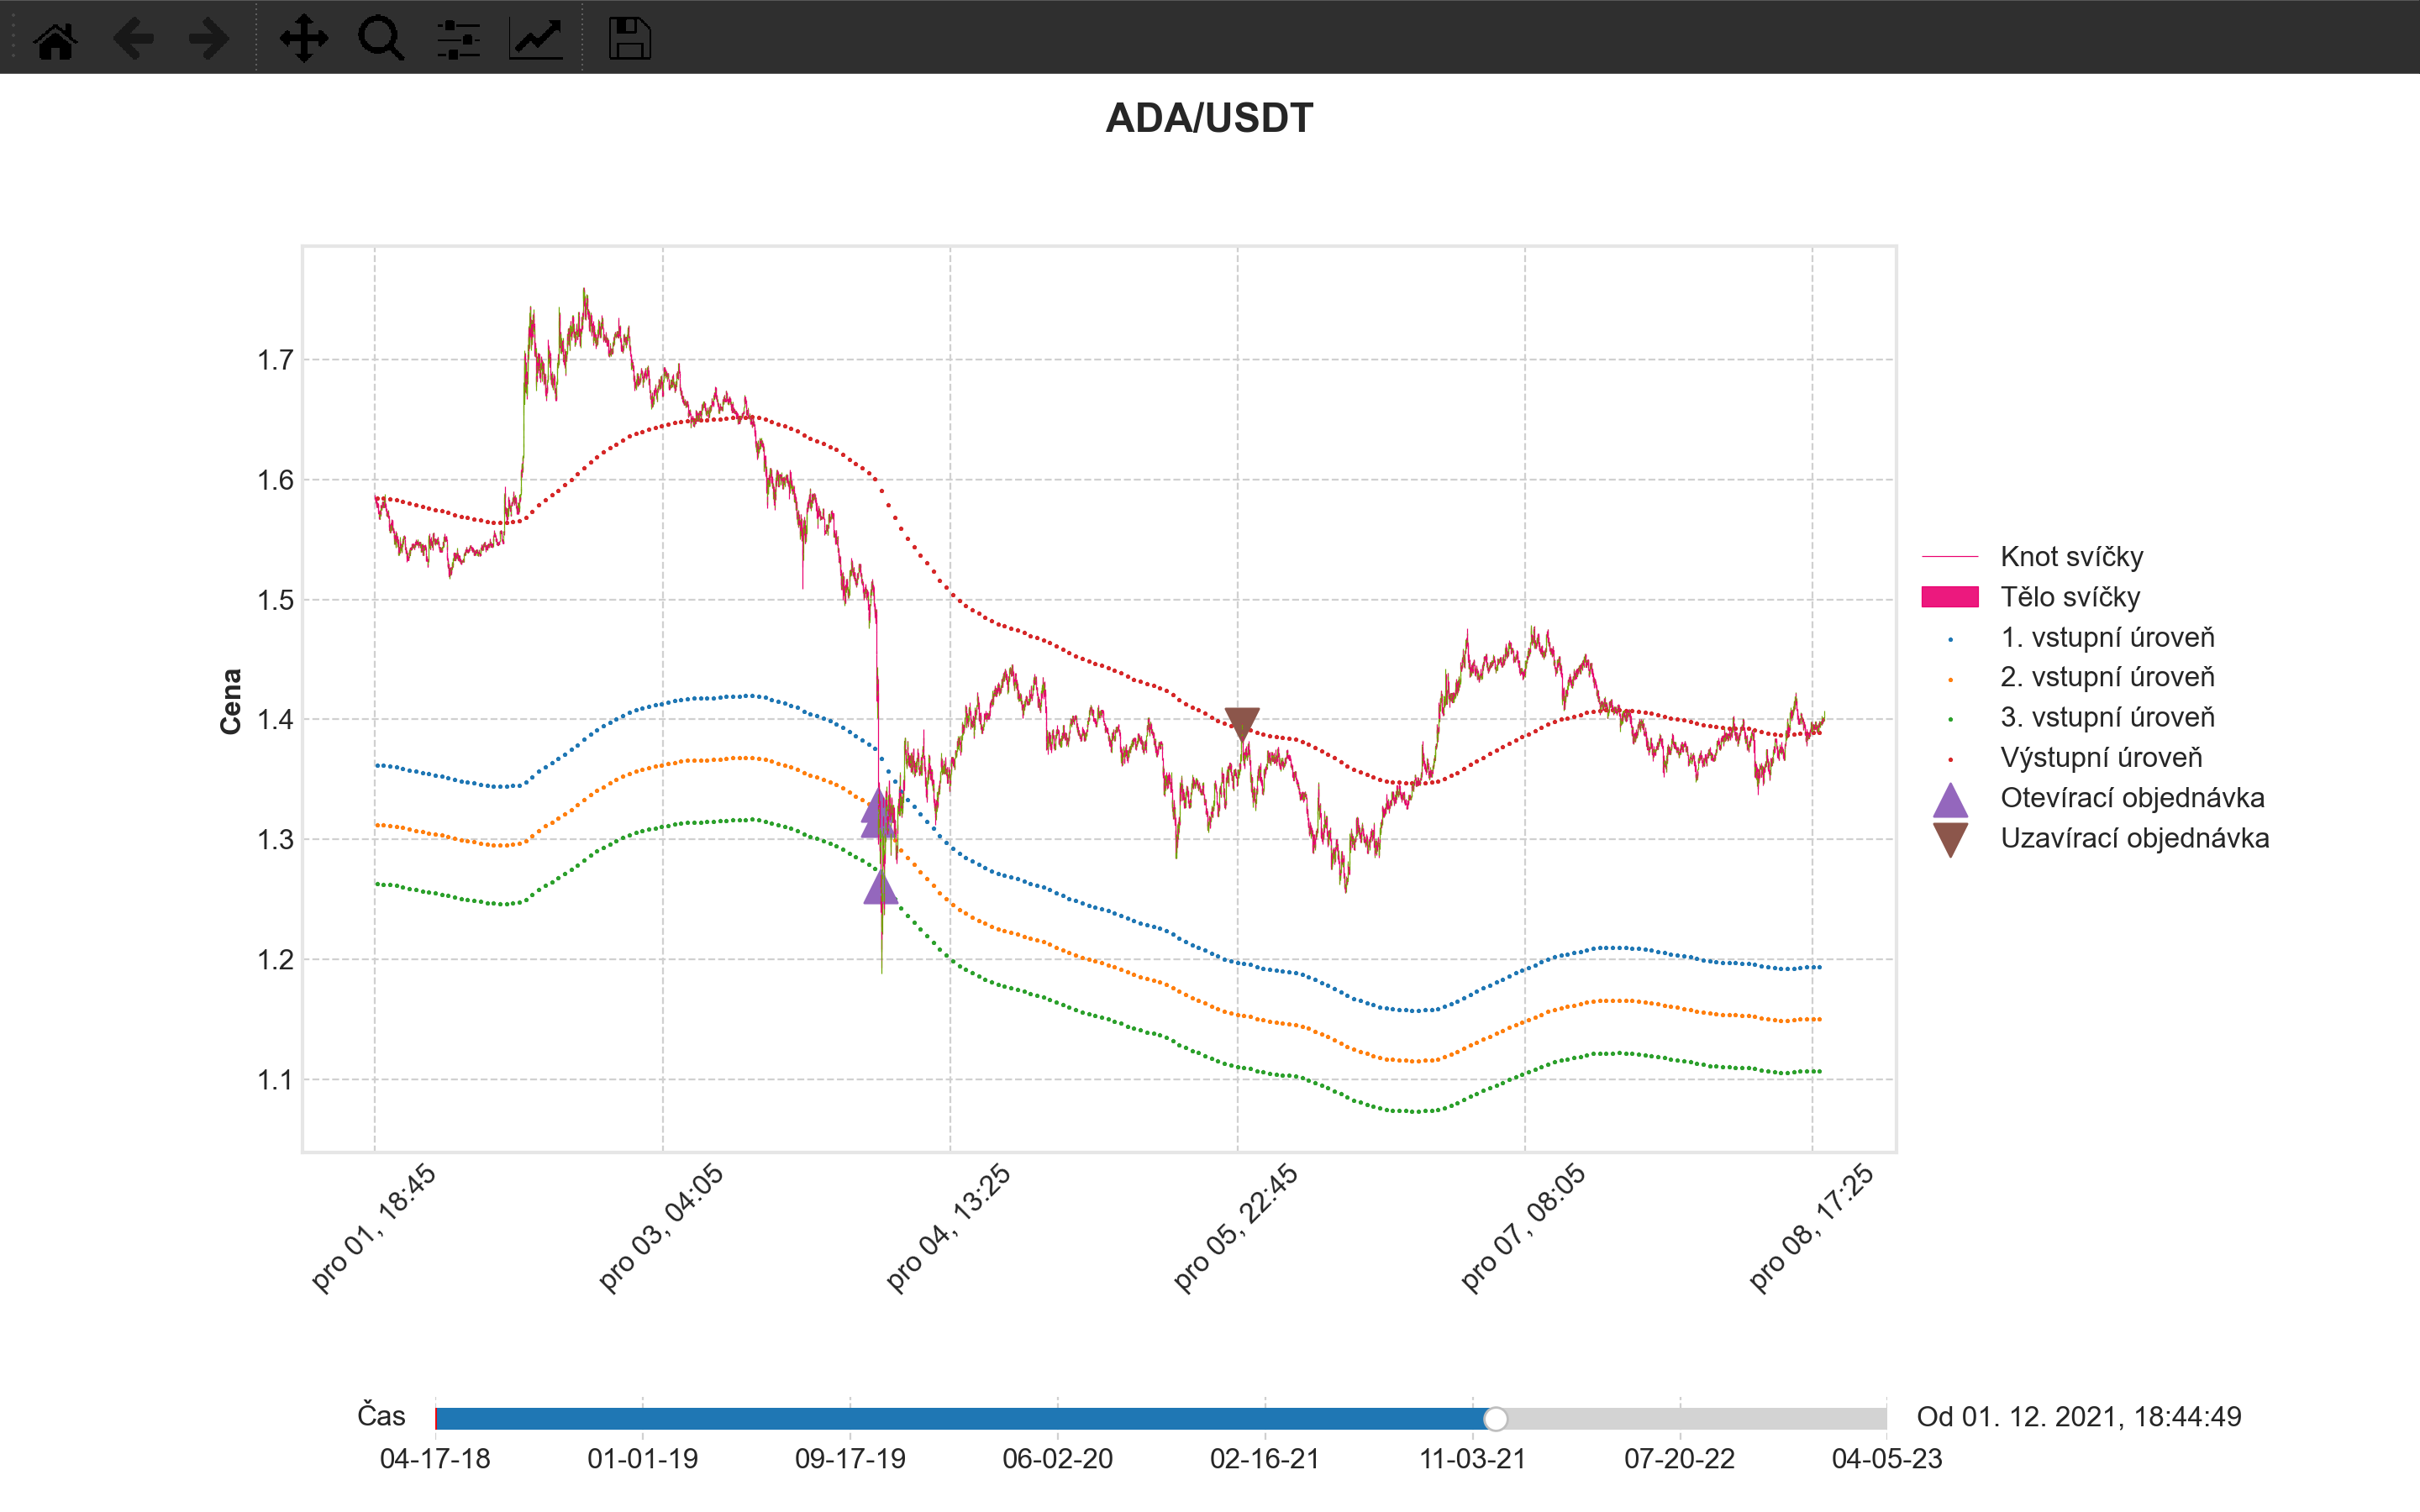
\includegraphics[scale=0.3]{img/historical-simulation-widget-2.png}}
\caption{Widget pro vykreslování svíček}
\label{fig:historical-simulation-widget}
\end{figure}

\chapter{Testování}
K zajištění správnosti kódu byly použity 2 nástroje, a to tvrzení (assertions) a unit testování.
Když něco vždy platí, lze to ověřit pomocí tvrzení.
V C++ jsou k dispozici makra z hlavičkového souboru \texttt{assert.h}.
Lze je například použít ke kontrole předpokladu, že vygenerované číslo je v požadovaném rozsahu.
Pokud neplatí, způsobí ukončení programu a nelze je zachytit jako výjimky.
Jejich cílem je zajistit, aby programátor neudělal chybu.
Mohou být použity ve fázi ladění a odstraněny, když je program připravený do produkce.
V C++ je lze snadno odstranit během kompilace pomocí příznaku \texttt{-DNDEBUG}.

Hlavním účelem výjimek je sdělit uživateli, proč program nemůže provést požadovanou úlohu.
Mohou být způsobeny například poskytnutím nesprávně naformátovaného CSV souboru s historickými svíčkovými daty, bez nichž program nemůže pokračovat.
Kontrola výjimečných stavů způsobuje režii navíc, takže se používají hlavně ve fázi konstrukce objektu, která se provádí pouze jednou.
Výjimky jsou vnořeny pomocí \texttt{std::throw\_with\_nested}, aby mohl uživatel získat co nejvíce informací k vyřešení problému.

V C++ existuje několik testovacích frameworků, ale Boost.Test a GoogleTest jsou 2, které vynikají nejvíce.
Oba používají makra k vytváření testovacích sad, testovacích případů a asercí, což minimalizuje množství práce potřebné k vytvoření testu.
Jsou dobře zdokumentované, široce používané a také integrované do IDE, jako je Visual Studio a CLion.
Pro tuto práci byl vybrán Boost.Test, protože je známější.

Testy jsou organizovány do testovacích modulů, které se skládají z testovacích sad obsahujících testovací případy.
Existuje několik způsobů, jak danou hierarchii vytvářet a používat.
Způsob vybraný pro projekt začíná vytvořením souboru \texttt{test.cpp}, který spojuje všechny moduly dohromady.
V souboru je jako první definováno makro \texttt{BOOST\_TEST\_MAIN} a pod ním jsou zahrnuty všechny moduly.
Na začátku každého modulu je nejprve zahrnut hlavičkový soubor frameworku.
Testovací sady a případy jsou vytvářeny pomocí maker.
Minimální příklad použití lze vidět na \ref{lst:test:module}.

\begin{lstlisting}[caption={~Ukázka testovacího modulu},label={lst:test:module},captionpos=t,abovecaptionskip=-\medskipamount,belowcaptionskip=\medskipamount,language=C]
#include <boost/test/unit_test.hpp>
#include <trading/ema.hpp>

BOOST_AUTO_TEST_SUITE(ema_test)
    BOOST_AUTO_TEST_CASE(default_constructor_test)
    {
        BOOST_REQUIRE_EQUAL(trading::ema{}.period(), std::size_t{1});
    }
    BOOST_AUTO_TEST_CASE(constructor_exception_test)
    {
        BOOST_REQUIRE_THROW(ema{0}, std::invalid_argument);
    }
    BOOST_AUTO_TEST_CASE(usage_test)
    {
        ma_usage_test<5,3,ema>({1, 2, 3, 7, 9}, {2.0, 4.5, 6.75}, 0.01);
    }
BOOST_AUTO_TEST_SUITE_END()
\end{lstlisting}

K samotnému testování jsou používány výroky (assertion), které jsou vyhodnoceny jako pravdivé nebo nepravdivé.
Framework nabízí různé výroky, které jsou spojeny s jednou ze tří úrovní testování.
Nejméně závažná je úroveň \texttt{WARN}, která vydá varovnou zprávu, pokud výrok není pravdivý.
Pokud je použita úroveň \texttt{CHECK}, vygeneruje chybu, ale umožní pokračovat v testování.
Nejzávažnější je úroveň \texttt{REQUIRE}, která vygeneruje chybovou hlášku a přeruší provedení daného testovacího případu.

Nabízí velmi dobře formátované a přehledné konzolové logy, které slouží k hlášení průběhu testování.
K dispozici jsou různé úrovně logování.
Ve výchozím nastavení je hlášeno vše: úspěch, varování, chyby, nezachycené výjimky a další.
Úroveň lze nastavit pomocí proměnné prostředí nebo příznaků příkazového řádku.

V CLion IDE lze testovací sady a případy spouštět jednotlivě.
Mohou být také spuštěny v režimu ladění.
Poskytuje různé nástroje, jak lépe prozkoumat výsledky testování.

\section{Strategie}
Strategie byla testována především proto, aby se zjistilo, zda byly správně implementovány podmínky pro vyvolání signálu.
Pro testování byl použit ukazatel typu SMA s periodou 1, jelikož je jeho hodnota rovna poslednímu předanému vzorku, což usnadňuje vytváření testů.
Každá metoda pro generování signálu vrací booleovskou hodnotu označující, zda má být vytvořena objednávka, čehož bylo využito při testování (viz \ref{lst:test:strategy:should:open}).
Byly také provedeny testy pro kontrolu inicializace, aktualizace indikátorů a metod pro získávání hodnot indikátorů.

\begin{lstlisting}[caption={~Testování podmínek pro signalizaci vytvoření otevírací objednávky},label={lst:test:strategy:should:open},captionpos=t,abovecaptionskip=-\medskipamount,belowcaptionskip=\medskipamount,language=C]
BOOST_AUTO_TEST_CASE(should_open_test)
{
    constexpr std::size_t n_levels{2};
    using indicator_t = trading::bazooka::indicator;
    using strategy_t = trading::bazooka::strategy<n_levels>;
    trading::sma entry{1}, exit{1};
    entry.update(10), exit.update(20);
    std::array<trading::fraction_t, n_levels> levels{{{2, 4}, {1, 4}}};
    strategy_t strategy(indicator_t{entry}, indicator_t{exit}, levels);

    // try open position above
    BOOST_REQUIRE_EQUAL(strategy.should_open(entry.value()*
        trading::fraction_cast<double>(levels[0])*1.001), false);
    BOOST_REQUIRE_EQUAL(strategy.next_entry_level(), 0);

    // open position
    BOOST_REQUIRE_EQUAL(strategy.should_open(entry.value()*
        trading::fraction_cast<double>(levels[0])), true);
    BOOST_REQUIRE_EQUAL(strategy.next_entry_level(), 1);
    ...
}
\end{lstlisting}

\section{Indikátory}
Hodnoty generované implementací indikátorů EMA a SMA byly porovnány s hodnotami generovanými knihovnou pro technickou analýzu TA-lib.
Pro testování byly použity různé hodnoty period a hodnot vzorků.
Otestováno bylo také, že při zavolání konstruktoru s neplatnými parametry, je vyhozena výjimka.
Byla zkontrolována správná indikace připravenosti indikátoru jak při zavolání metody \texttt{update} tak \texttt{is\_ready}.

\section{Manažer}
Manažer přijímá signály generované strategií a převádí je na objednávky, které jsou následně předány burze.
I když je to složitější třída, tak lze její stav simulovat zvenčí.
Proto byly při testování pro srovnání stavu trhu použity očekávané instance tříd \texttt{market}, \texttt{wallet}, \texttt{order\_sizer}, \texttt{open\_order} a \texttt{close\_all\_order}.
Nejprve byla zkontrolována správná inicializace třídy a poté byl proveden test použití.

Během testování byly volány metody pro vytváření tržních objednávek k otevření, zvýšení a uzavření pozice.
V každé fázi byly nejprve vypočítány očekávané objednávky, které byly použity k aktualizaci očekávaného trhu.
Objednávky bylo možné porovnat se skutečnými objednávkami pomocí metod pro přístup k posledním objednávkám, jako je \texttt{last\_open\_order}.
Jakmile byly tržní stavy identické, mohly být k jejich porovnání použity metody přístupu k tržnímu stavu jako \texttt{wallet\_balance}.

\section{Obchodník}
Třída \texttt{trader} spojuje funkcionality strategie a manažera.
Implementuje jedinou metodu, která rozhoduje, kdy obchodovat.
Jelikož třída přebírá manažera a strategii jako šablonové argumenty, mohly by být zaměněny za falešné (mock) objekty.
Objekty jsou velmi jednoduché, implementují dané rozhraní a jejich atributy jsou typu boolean.
Atributy se používají k nastavení výsledků volání metod.
Implementaci falešné strategie lze vidět na výpisu \ref{lst:mock:strategy}.
Tímto způsobem mohly být snadno otestovány všechny možné scénáře.

\begin{lstlisting}[caption={~Implementace falešná strategie},label={lst:mock:strategy},captionpos=t,abovecaptionskip=-\medskipamount,belowcaptionskip=\medskipamount,language=C]
struct mock_strategy {
    bool ready{false}, open{false}, close_all{false};

    bool is_ready() const { return ready; }

    bool should_open(trading::price_t) const { return open; }

    bool should_close_all(trading::price_t) const { return close_all; }
};
\end{lstlisting}

\section{Burza}
Třída \texttt{market} byla nejprve testována na správnou inicializaci a výjimky, které mohou být vyvolány při volání konstruktoru.
Konstruktor vyvolá výjimku typu \texttt{std::invalid\_argument}, když je mu předána neplatná hodnota poplatku.
Aby bylo možné otestovat její použití, byly k porovnání hodnot udržovány instance tříd \texttt{position} a \texttt{wallet} představují očekávaný stav třídy.
Test prošel všemi stavy aktivní pozice: vytvoření, navýšení a uzavření, během kterých byly skutečné hodnoty poskytované metodami třídy porovnány s očekávanými.

\section{Pozice}
Nejprve byla testována inicializace pro kontrolu, že jsou všechny atributy správně inicializovány.
Hlavním provedeným testem byl test použití, během kterého byla pozice otevřena, navýšena a uzavřena.
Během testu byly počítány očekávaná celková investovaná částka a očekávaná velikost pozice pro kontrolu výsledků volání metod a stavu atributů pozice.

\section{Simulátor}
Cílem prvního testu bylo ujistit se, že proces převzorkování prováděný v těle konstruktoru je správně implementován.
Za tímto účelem byly vypočteny očekávané ceny a indikátorové ceny a porovnány s hodnotami získanými pomocí getrů instanciované třídy.
Poté byla testována samotná simulace přístupná pomocí volacího operátoru třídy, který přebírá 2 typy parametrů: obchodníka a sadu pozorovatelů.
Ke kontrole, zda jsou pozorovatelé voláni správně, byl použit pozorovatel počítající počet událostí.
Jako obchodník byla použita mockovací třída, která umožňovala nastavení výsledků volání metod před použitím simulátoru.
Pomocí těchto 2 objektů bylo provedeno několik testovacích případů.

\section{Statistiky}
Výkonnostní statistiky byly testovány, aby bylo zajištěno, že jsou hodnoty správně inicializovány a aktualizovány.
Bylo využito toho, že jsou rozděleny do 4 nezávislých skupin: statistiky související s pohybem, statistiky související se ziskem, čítače otevřených a uzavřených objednávek a zůstatky.
Na všech byly proto provedeny samostatné testovací případy.

\section{Generátory stavového prostoru}
Generátory byly testovány na výjimky, které generují pro neplatný vstup.
Hodnoty generované systematickými generátory byly zkontrolovány na platnost a jedinečnost a porovnány se sadou očekávaných hodnot.
Současně byly použity různé kombinace hodnot parametrů.
Jakmile byla získána určitá úroveň důvěry, byly systematické generátory použity k testování náhodných generátorů.
Hlavním cílem byla kontrola dosažitelnosti, pokud náhodné generátory vygenerovaly všechny možné hodnoty v určitém počtu iterací, byly považovány za validní \ref{lst:test:reachability}.

\begin{lstlisting}[caption={~Testování dosažitelnosti stavů},label={lst:test:reachability},captionpos=t,abovecaptionskip=-\medskipamount,belowcaptionskip=\medskipamount,language=C]
template<class Value, class SystematicGenerator, class RandomGenerator>
void test_reachability(Value origin, SystematicGenerator&& sys_gen,
    RandomGenerator&& rand_gen, std::size_t n_it)
{
    std::size_t it{0};
    using map_type = std::map<Value, std::size_t>;
    map_type options;

    for (const auto& value: sys_gen())
        options.insert(typename map_type::value_type{value, 0});

    while (it++!=n_it) {
        origin = rand_gen(origin);
        BOOST_REQUIRE(options.contains(origin));
        options[origin] += 1;
    }

    for (const auto& [opt, count]: options)
        BOOST_REQUIRE(count);
}
\end{lstlisting}

\section{Optimalizátory}
Optimalizátory nabízejí vysokou úroveň abstrakce díky použití konceptů a šablon, takže pro jejich testování mohl být použit integer jako typ konfigurace, což značně zjednodušilo testy.
Pro generování stavového prostoru mohly být využity generátory  \texttt{systematic::int\_range\_generator} a \texttt{random::int\_range\_generator}.

Jako objektivní funkce byla zvolena funkce převádějící integer na double.
Cílem všech testů bylo nalézt její maximální hodnotu.
Omezení mohla být definována uvedením minimální objektivní hodnoty.
Byly testovány na výjimky, které by mohly být vyvolány během inicializace objektu.
Aby bylo možné zkontrolovat, zda jsou pozorovatelé informováni o událostech správně, byli vytvořeni pozorovatelé pro počítání událostí.
Ukázku testování simulovaného ochlazování pomocí čítacího pozorovatele lze vidět na \ref{lst:test:event:counter}.

\begin{lstlisting}[caption={~Testování optimalizátoru pomocí pozorovatele},label={lst:test:event:counter},captionpos=t,abovecaptionskip=-\medskipamount,belowcaptionskip=\medskipamount,language=C]
BOOST_AUTO_TEST_CASE(count_events_test)
{
    using config_t = int;
    using optimizer_t =trading::simulated_annealing::optimizer<config_t>;
    using state_t = optimizer_t::state_type;
    double start_temp{100}, min_temp{1};
    auto cooler = [](auto& optimizer) {
        optimizer.current_temperature(optimizer.current_temperature()-1);
    };
    auto appraiser = [](const auto& current, const auto& candidate) {
        return current.value-candidate.value;;
    };
    auto objective = [](const auto& config) {
        return static_cast<double>(config);
    };
    auto constraints = [](const state_t& candidate) { return true; };
    auto neighbor = trading::random::int_range(1, 100, 1);
    auto equilibrium=trading::simulated_annealing::fixed_equilibrium{10};
    auto optimizer = optimizer_t{start_temp, min_temp};
    auto counter = event_counter{};
    int init_value{neighbor()};
    state_t init{init_value, objective(init_value)};
    trading::constructive_result result{init,
        [&](const auto& lhs, const auto& rhs) {
        return lhs.value>rhs.value;
    }};
    optimizer(init.config, result, constraints, cooler,
        objective, neighbor, appraiser, equilibrium, counter);
    BOOST_REQUIRE_EQUAL(counter.started_count, 1);
    BOOST_REQUIRE_EQUAL(counter.finished_count, 1);
    BOOST_REQUIRE_EQUAL(counter.cooled_count, optimizer.it());
    BOOST_REQUIRE(counter.better_accepted_count>0);
    BOOST_REQUIRE(counter.worse_accepted_count>0);
}
\end{lstlisting}

\subsection{Hrubá síla}
Optimalizátor hrubé síly byl nejsnáze testovatelný.
Vyhledávací prostor byl generován pomocí systematicky, takže optimalizátor vždy najde nejlepší stav.
Testováno bylo také použití omezení a procházení prázdného vyhledávacího prostoru.

\subsection{Simulované ochlazování}
Třída \texttt{simulated\_annealing::optimizer} byla nejprve testována na správnou inicializaci a výjimky, které jsou vyvolány při předání neplatných hodnot.
Ke kontrole, zda byli pozorovatelé správně informováni o událostech, byl použit čítač událostí.
Jednotlivé čítače událostí byly kontrolovány během optimalizace uvnitř metod čítače (viz \ref{lst:event:counter:finished}) a nakonec po jejím skončení.
Hledání závisí na náhodném prohledávání sousedních stavů, takže test použití byl nastaven tak, aby po dostatečném množství iterací bylo nalezení nejlepšího stavu téměř jisté.

\begin{lstlisting}[caption={~Kontrola hodnot čítače uvnitř metody \texttt{finished}},label={lst:event:counter:finished},captionpos=t,abovecaptionskip=-\medskipamount,belowcaptionskip=\medskipamount,language=C]
template<class Optimizer>
void finished(const Optimizer&)
{
    BOOST_REQUIRE_EQUAL(started_count, 1);
    BOOST_REQUIRE_EQUAL(finished_count, 0);
    finished_count++;
}
\end{lstlisting}

\subsection{Genetický algoritmus}
Třída \texttt{genetic\_algorithm::optimizer} byla testována velmi podobně.
Operátor křížení byl implementován jako průměr konfigurací 2 rodičů.
Mutace byla provedena stejně, pouze druhý rodič byl generován náhodně.
Byly navrženy 2 testovací případy pro kontrolu \texttt{bazooka::crossover} třídy.
Cílem prvního bylo se ujistit, že pokud jsou rodiče stejní, tak je totožné i jejich dítě.
Při druhém byli opakovaně vygenerováni náhodní rodiče a bylo zkontrolováno, že produkují validní potomky.

\subsection{Tabu prohledávání}
Třída \texttt{int\_range\_memory} byla použita jako paměť pro testování \texttt{tabu\_search::optimizer}.
Jinak testování probíhalo stejně jako u ostatních optimalizátorů.
Paměťové třídy byly také testovány, aby bylo zajištěno, že si správně pamatují a zapomínají hodnoty, které jim byly předány.

\section{Čtení a zápis do CSV}
Pro testování čtení a zápisu do CSV souborů byly připraveny 4 soubory: prázdný, pouze s hlavičkou, pouze s daty a kompletní soubor.
Při použití čtecí třídy může být vyvolána výjimka \texttt{std::runtime\_error}, buď při volání konstruktoru, pokud soubor neexistuje, nebo při samotném čtení, pokud je soubor nesprávně naformátován nebo je třída nesprávně používána.
Rozlišuje mezi výjimkou, která nastane při oddělování dat oddělovačem, a výjimkou, která nastane při převodu dat na požadovaný datový typ.
Hlavním rozdílem mezi nimi je obsah chybové zprávy.
Byly provedeny důkladné testy k simulaci požadovaných a výjimečných situací.
Třída čtení byla použita k testování třídy zápisu, aby se ověřilo, že produkuje validní výstup.

\chapter{Experimentální vyhodnocení}
Cílem experimentálního vyhodnocení bylo najít vhodná nastavení pro optimalizátory a mít možnost je vzájemně porovnat.
Experimenty byly prováděny systematicky tak, že nejprve bylo nalezeno nejlepší nastavení pro jednu sadu historických dat a poté několik málo dalších.
Tímto způsobem byla provedena fáze hodnocení white-box následovaná fází black-box, během které byla pro hodnocení použita historická data, která byla dříve neznámá.
Výsledky experimentů byly pečlivě a systematicky uchovávány, aby bylo co nejjednodušší rozhodování, co upravit pro další experiment.

Výsledky experimentů jsou umístěny v systematicky uspořádané hierarchii složek.
Všechny mají společný adresář výstupních dat, který obsahuje 4 složky s názvy odpovídajícími jednotlivým optimalizátorům, do nichž patří složky s výsledky jednotlivých experimentů.
Názvy složek s výsledky jsou čísla podle pořadí, ve kterém byl daný experiment proveden.
Například výsledky 1. experimentu genetického algoritmu lze nalézt ve složce \textit{data/out/genetic-algorithm/01}.

Výsledky všech experimentů se skládají z minimálně 3 souborů: log.txt, best-states.json a settings.json.
Soubor log.txt obsahuje zprávy, které byly během procesu optimalizace zobrazeny do konzole.
Aby bylo možné výsledky zobrazit na standardní výstup a zároveň je zapsat do souboru, byl použit \texttt{boost::iostreams::stream} spolu s \texttt{boost::iostreams::tee\_device}.
Všechny optimalizátory mají společný začátek logu s informacemi o načtených historických datech \ref{lst:log:candles}.

\begin{lstlisting}[caption={~Informace o načtených historických svíčkách z výstupního logu},label={lst:log:candles},captionpos=t,abovecaptionskip=-\medskipamount,belowcaptionskip=\medskipamount,language=C]
candles read:
from: 2017-Aug-17 04:00:00
to: 2022-Oct-28 12:27:00
difference: 1898d 08:27:00.000000
count: 2725146
duration: 3.664928s
\end{lstlisting}

Nastavení experimentu jsou uložena do souboru JSON.
Díky tomu je experiment opakovatelný, i když výsledky nemusí být stejné, alespoň to platí pro všechny heuristické optimalizátory, protože spoléhají na randomizaci.
Všechny optimalizátory mají společné sekce nastavení.
Obsahují informace o historických datech, převzorkování a vyhledávacím prostoru \ref{lst:common:settings}.

\begin{lstlisting}[caption={~Společné části nastavení},label={lst:common:settings},captionpos=t,abovecaptionskip=-\medskipamount,belowcaptionskip=\medskipamount,language=C]
{
    "candles": {
        "count": 2160979,
        "currency pair": {
            "base": "ZRX",
            "quote": "USDT"
        },
        "from": 1551326400,
        "to": 1681230420
    },
    "optimization criterion": "prom",
    "resampling": {
        "averaging method": "ohlc4",
        "period[min]": 15
    },
    "search space": {
        "indicator": {
            "period": {
                "from": 3,
                "step": 3,
                "to": 105
            },
            "types": [
                "sma"
            ]
        },
        "levels": {
            "count": 3,
            "lower bound": "12/20",
            "unique count": 15
        },
        "open order sizes": {
            "unique count": 11
        }
    }
}
\end{lstlisting}

Nejlepší stavy jsou uloženy jako seznam konfigurací a statistik v souboru best-states.json.
K dispozici jsou různé statistiky, které mohou pomoci lépe porozumět chování optimalizované strategie \ref{lst:best-state}.

\begin{lstlisting}[caption={~Informace uložené o nejlepším stavu},label={lst:best-state},captionpos=t,abovecaptionskip=-\medskipamount,belowcaptionskip=\medskipamount]
{
    "configuration": {
        "indicator": {
            "period": 36,
            "type": "ema"
        },
        "levels": ["5/6","4/6","2/6"],
        "open sizes": ["5/7","1/7","1/7"]
    },
    "statistics": {
        "close balance": {
            "max": 78961.828125,
            "max drawdown": {
                "amount": -459.23828125,
                "percent": -1.4765747785568237
            },
            "max run up": {
                "amount": 68961.828125,
                "percent": 689.6182861328125
            },
            "min": 10000.0
        },
        "equity": {
            "max": 78961.828125,
            "max drawdown": {
                "amount": -11520.890625,
                "percent": -34.7911491394043
            },
            "max run up": {
                "amount": 69040.4375,
                "percent": 695.8746337890625
            },
            "min": 9921.390625
        },
        "gross loss": -459.23828125,
        "gross profit": 69421.0625,
        "net profit": 68961.828125,
        "open order counts": [24,2,0],
        "order ratio": 1.0833333333333333,
        "profit factor": 151.16566467285156,
        "total close orders": 24,
        "total open orders": 26
    }
},
\end{lstlisting}

Python skripty byly následně použity k vytvoření souhrnných tabulek a grafů z dat generovaných optimalizací.
Tímto způsobem bylo následné zpracování automatizováno, což snížilo možnost udělat chybu a výrazně zkrátilo čas potřebný k vytvoření přehledových tabulek.

Experimenty byly prováděny na notebooku MacBook Pro s 2,3 GHz Intel 4jádrovým procesorem s 32 GB RAM pamětí.
Procesor podporuje hyper-trading, který umožňuje současný běh 2 vláken na každém jádru.
Což ovlivňuje framework OpenMP, který díky tomu může používat 8 vláken.

\section{Historická data}
Data pro experimenty byla získána ze stránky CryptoArchive (www.cryptoarchive.com.au).
Data pocházejí z Binance kryptoměnové burzy a jsou aktualizována denně.
Mezi hlavní důvody, proč byl web upřednostněn před ostatními dostupnými poskytovateli, patřilo to, že data byla zdarma, snadno dostupná a v požadované granularitě.

Bylo vybráno 10 různých kryptoměn včetně některých známějších jako Bitcoin (BTC), Ethereum (ETH) a Litecoin (LTC) a také novějších jako Solana (SOL).
Pokrývají 2,7--5,7 let historie, což stačí k zachycení různých tržních trendů.
Například v případě Bitcoinu pokrývá nárůst ceny na konci roku 2017 a 2022, jakož i její pokles na začátku roku 2019 a 2023.
Hodnoty kryptoměn jsou uvedeny v USDT, což je stablecoin, jehož hodnota se blíží americkému dolaru.
Přehled informací o vybraných historických datech je uveden v tabulce \ref{tab:historical:market:data}.

\begin{table}[!htbp]
\centering
\centering
\caption[Přehled historických dat]{~Přehled historických dat}\label{tab:historical:market:data}
{%
\begin{tabular}{|l|c|c|c|c|}
\hline
\multicolumn{1}{|c|}{\textbf{Měna}} & \textbf{Počet svíček} & \textbf{Od (den)} & \textbf{Do (den)} & \textbf{Doba (roky)} \\ \hline
ADA  & 2 616 803 & 17. 04. 2018 & 12. 04. 2023 & 5,0 \\ \hline
BTC  & 2 963 250 & 17. 08. 2017 & 11. 04. 2023 & 5,7 \\ \hline
DASH & 2 122 039 & 28. 03. 2019 & 12. 04. 2023 & 4,0 \\ \hline
DOGE & 1 979 751 & 05. 07. 2019 & 12. 04. 2023 & 3,8 \\ \hline
ETH  & 2 963 365 & 17. 08. 2017 & 12. 04. 2023 & 5,7 \\ \hline
LTC  & 2 794 419 & 13. 12. 2017 & 12. 04. 2023 & 5,3 \\ \hline
SOL  & 1 400 292 & 11. 08. 2020 & 11. 04. 2023 & 2,7 \\ \hline
XLM  & 2 552 037 & 31. 05. 2018 & 11. 04. 2023 & 4,9 \\ \hline
XRP  & 2 591 038 & 04. 05. 2018 & 11. 04. 2023 & 4,9 \\ \hline
ZRX  & 2 160 979 & 28. 02. 2019 & 11. 04. 2023 & 4,1 \\ \hline
\end{tabular}%
}
\end{table}

Průměrná doba výpočtu objektivní funkce je přibližně 0,006 sekundy, což znamená, že prohledání 1 milionu různých stavů by trvalo přibližně 1,5 hodiny.
Výpočet byl proveden na mnohem větším vyhledávacím prostoru pro získání přesnějších výsledků.

\section{Hrubá síla}
Hlavním účelem algoritmu hrubé síly bylo vyzkoušet použití různých optimalizačních kritérií a omezení.
Je to také dobrý způsob měření vlivu optimalizace.
Může to být jednoduché a dostatečně efektivní řešení pro optimalizaci na malém vyhledávacím prostoru pro jednodušší strategie.
Nebylo potřeba provádět white-box ani black-box vyhodnocení, protože optimalizátor nemá žádné nastavitelné parametry.

Log byl doplněn o informace o celkovém počtu stavů prohledávaného stavového prostoru a čase zahájení a ukončení optimalizace (viz \ref{lst:brute:force:log}).
Časy byly získány a naformátovány pomocí funkce z knihovny Boost.DateTime.
Celkový počet stavů byl vypočten procházením vyhledávacího prostoru, což u malých vyhledávacích prostorů nezabere ve srovnání s dobou optimalizace významné množství času.

\begin{lstlisting}[caption={~Rozšíření logu pro algoritmus hrubé síly},label={lst:brute:force:log},captionpos=t,abovecaptionskip=-\medskipamount,belowcaptionskip=\medskipamount]
periods count: 35
tag count: 1
levels count: 455
sizes count: 66
total count: 1051050
began: 2023-Apr-16 05:16:06
ended: 2023-Apr-16 06:20:26
duration: 01:04:20.000111
\end{lstlisting}

\subsection{Optimalizace}
První experimenty, které byly provedeny byly zaměřeny na měření účinků optimalizací.
Byly použity 2 typy optimalizací: optimalizace kompilátoru a paralelismus.
Hlavní použitá optimalizace kompilátoru byla \texttt{O3}, která nastavuje nejvyšší úroveň optimalizací.
Druhou je \texttt{march=native}, která říká kompilátoru, aby provedl optimalizaci pro konkrétní CPU na daném počítači.

Dopad těchto optimalizací byl znatelný, protože sekvenční implementace se zapnutými optimalizacemi byla \textbf{11krát} rychlejší než ta bez nich.
Použitím paralelismu byl algoritmus ještě \textbf{3,6krát} rychlejší s 8 vlákny.
Porovnání výsledků experimentu s vyhledávacím prostorem skládajícím se z 3600 stavů a simulací běžící na 2,5 milionu minutových svíček si lze prohlédnout v tabulce \ref{tab:brute:force:optimization}.

\begin{table}[!htbp]
\centering
\caption[Vliv použití optimalizace]{~Vliv použití optimalizace}\label{tab:brute:force:optimization}
\begin{tabular}{|l|l|l|}
\hline
\textbf{Optimalizace}                  & \textbf{Doba trvání (s)} & \textbf{Zrychlení} \\ \hline
žádné                                   & 986                      & 1                                                     \\ \hline
optimalizace kompilátoru                & 88                       & 11,2                                                  \\ \hline
optimalizace kompilátoru a paralelismus & 24                       & 41,1                                                   \\ \hline
\end{tabular}
\end{table}

\subsection{Experimenty}
Na začátku bylo provedeno několik experimentů k nalezení vhodného vyhledávacího prostoru.
Hodnoty úrovně nákupu se ukázaly být nejdůležitějším konfiguračním parametrem, který musel mít širokou škálu možných hodnot.
Ke generátorům úrovně nákupu byl přidán parametr spodní hranice, čímž se snížil počet jedinečných hodnot potřebných k nalezení přijatelných výsledků, a tím se zmenšil vyhledávací prostor.

PROM byl zvolen jako optimální kritérium, jelikož poskytuje rozumné výsledky s vyváženým poměrem rizika a zisku.
Byla také vyzkoušena jiná jednodušší optimalizační kritéria, jako maximalizace ziskového faktoru, což vedlo k nalezení konfigurací, které byly velmi bezpečné, avšak přinášely nízké zisky.

Výsledky byly primárně porovnávány pomocí statistik, nicméně byla použita i vizualizace.
Na grafu \ref{fig:btc-historical-simulation} lze vidět, že strategie obchoduje, když dochází k rychlým poklesům ceny.
Při vhodném nastavení přináší zisky, ale může se stát, že strategie otevře pozici příliš brzy, což vede k nižším ziskům nebo dokonce ztrátám.
Stalo by se to například na začátku roku 2020, kdy začala pandemie COVID, následky jsou vidět na grafu s čistou hodnotou.
Je také vidět, že většina obchodů byla provedena na začátku kolem roku 2018 a počet obchodů s postupem času klesá, což může naznačovat, že strategie byla optimalizována na příliš velkém množství dat nebo není vhodná pro obchodování daného aktiva.

\begin{figure}[htbp]
\centerline{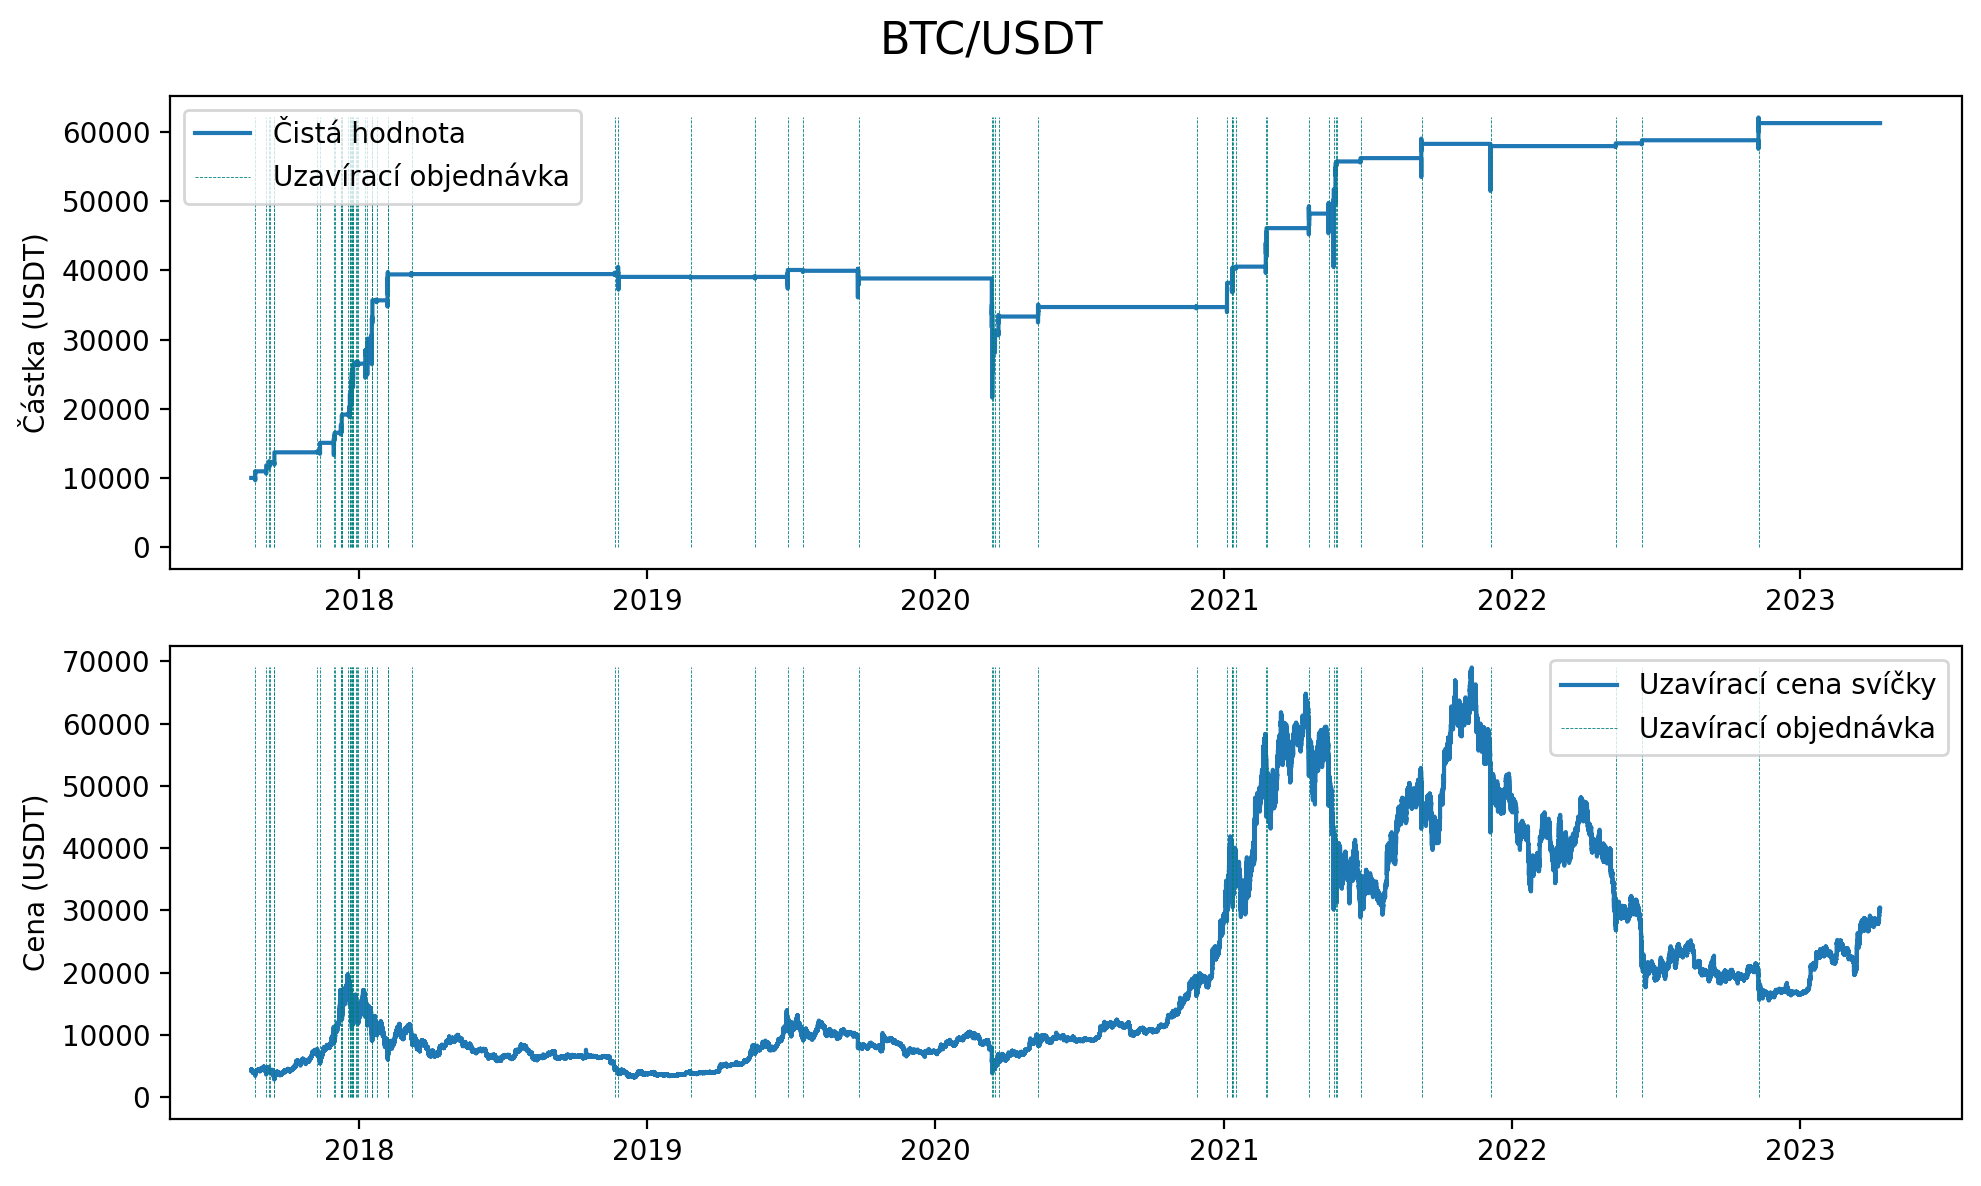
\includegraphics[scale=0.6]{img/btc-historical-simulation.png}}
\caption{Průběh historické simulace BTC}
\label{fig:btc-historical-simulation}
\end{figure}

Po dokončení počátečních testů byly provedeny 2 sady testů na všech historických datech.
Hodnoty parametrů generátorů vyhledávacího prostoru byly zvoleny na základě získaných výsledků.
I při použití optimalizace byl čas stále limitujícím faktorem.
Rozumná velikost vyhledávacího prostoru se pohybuje 0,5--1 milion možných konfigurací, což trvá přibližně 1--1,5 hodiny, než se dokončí jeden běh optimalizace, a protože bylo zvoleno 10 aktiv, trvala 1 sada experimentů 10--15 hodin.

Sady experimentů měly přibližně 1 milion možných konfigurací.
Hodnoty parametrů generátorů stavového prostoru a perioda převzorkování jsou uvedeny v tabulce \ref{tab:brute:force:sets:search:space}.
Změny provedené po 1. sadě experimentů spočívaly v tom, že počet jedinečných hodnot úrovní nákupu byl zvýšen z 15 na 20 a v seznamu možných typů ukazatelů byl ponechán pouze SMA.
Během poslední sady experimentů byla doba převzorkování zkrácena ze 45 minut na 15, počet jedinečných hodnot úrovní nákupu byl vrácen na zpět 15, byl zvýšen počet jedinečných hodnot velikostí nákupu z 6 na 11 a spodní hranice úrovní nákupu byla snížena z \(-20 \%\) na \(-40 \%\).

\begin{table}[!htbp]
\centering
\caption[Přehled hodnot parametrů vyhledávacího prostoru pro sady experimentů]{~Přehled hodnot parametrů vyhledávacího prostoru pro sady experimentů}
\label{tab:brute:force:sets:search:space}
\resizebox{\textwidth}{!}{%
\begin{tabular}{|l|c|c|c|c|c|c|c|c|}
\hline
\multicolumn{1}{|c|}{\textbf{Sada}} &
  \textbf{\begin{tabular}[c]{@{}c@{}}Období\\ převzorkování\end{tabular}} &
  \textbf{\begin{tabular}[c]{@{}c@{}}Úrovně nákupu\\ počet jedinečných hodnot\end{tabular}} &
  \textbf{\begin{tabular}[c]{@{}c@{}}Úrovně nákupu\\ spodní hranice (\%) \end{tabular}} &
  \textbf{\begin{tabular}[c]{@{}c@{}}Velikosti nákupu\\ počet jedinečných hodnot\end{tabular}} &
  \textbf{\begin{tabular}[c]{@{}c@{}}Období\\ od\end{tabular}} &
  \textbf{\begin{tabular}[c]{@{}c@{}}Období\\ do\end{tabular}} &
  \textbf{\begin{tabular}[c]{@{}c@{}}Období\\ krok\end{tabular}} &
  \textbf{Ukazatelé} \\ \hline
1 & 45 & 15 & \(-25,0\) & 6  & 3 & 60  & 3 & \([\begin{array}{cc} SMA & EMA \end{array}]\) \\ \hline
2 & 15 & 15 & \(-40,0\) & 11 & 3 & 105 & 3 & \([\begin{array}{c} SMA \end{array}]\)        \\ \hline
\end{tabular}%
}
\end{table}

Hodnoty úrovně nákupu a velikosti nákupu byly převedeny ze zlomků do čitelnějšího formátu.
Obě jsou uvedeny v procentech, úrovně jsou záporné a udávají, o kolik je úroveň snížena od hodnoty vstupního indikátoru, a velikosti označují část zůstatku na účtu, která je použita k nákupu na dané úrovni.

Z přehledu nejlepších konfigurací z 1. sady experimentů (viz \ref{tab:brute:force:set:1:best:configs}) lze vidět, že 8 z 10 distribucí úrovně nákupu klade důraz na jednu úroveň nákupu tím, že na ni vloží 75 \% zůstatku a minimum možné na zbytek.
Na základě toho by se měl zvýšit počet jedinečných velikostí, aby byla dostupná větší rozmanitost distribucí.
Medián první úrovně nákupu je \(-12.5 \% \) a poslední úrovně \( -19.6 \% \). 
Poslední úroveň je velmi blízko spodní hranici úrovně nákupu, což naznačuje, že může být výhodné ji snížit ještě více.
SMA je přítomen v 7 z 10 nejlepších konfigurací, takže indikátor EMA lze v dalších experimentech vynechat.
V případě měny XLM dosáhlo maximální hodnoty období, což naznačuje, že by měla být maximální hodnota zvýšena.

% Please add the following required packages to your document preamble:
% \usepackage{graphicx}
\begin{table}[!htbp]
\centering
\caption[Přehled nejlepších konfigurací z 1. sady experimentů]{~Přehled nejlepších konfigurací z 1. sady experimentů}\label{tab:brute:force:set:1:best:configs}
{%
\begin{tabular}{|l|c|c|c|c|}
\hline
\multicolumn{1}{|c|}{\textbf{Měna}} & \textbf{Ukazatel} & \textbf{Období} & \textbf{Nákupní úrovně (\%)} & \textbf{Nákupní velikosti (\%)} \\ \hline
ADA  & EMA & 51 & \([\begin{array}{ccc} -14,1 & -17,2 & -20,3 \end{array}]\) & \([\begin{array}{ccc} 12,5 & 12,5 & 75,0 \end{array}]\) \\ \hline
BTC  & SMA & 15 & \([\begin{array}{ccc} -9,4 & -10,9 & -12,5 \end{array}]\)  & \([\begin{array}{ccc} 12,5 & 75,0 & 12,5 \end{array}]\) \\ \hline
DASH & SMA & 15 & \([\begin{array}{ccc} -14,1 & -17,2 & -18,8 \end{array}]\) & \([\begin{array}{ccc} 12,5 & 75,0 & 12,5 \end{array}]\) \\ \hline
DOGE & SMA & 15 & \([\begin{array}{ccc} -12,5 & -20,3 & -21,9 \end{array}]\) & \([\begin{array}{ccc} 25,0 & 12,5 & 62,5 \end{array}]\) \\ \hline
ETH  & SMA & 18 & \([\begin{array}{ccc} -14,1 & -15,6 & -17,2 \end{array}]\) & \([\begin{array}{ccc} 75,0 & 12,5 & 12,5 \end{array}]\) \\ \hline
LTC  & EMA & 12 & \([\begin{array}{ccc} -10,9 & -12,5 & -14,1 \end{array}]\) & \([\begin{array}{ccc} 12,5 & 12,5 & 75,0 \end{array}]\) \\ \hline
SOL  & EMA & 9  & \([\begin{array}{ccc} -7,8 & -12,5 & -17,2 \end{array}]\)  & \([\begin{array}{ccc} 12,5 & 62,5 & 25,0 \end{array}]\) \\ \hline
XLM  & SMA & 60 & \([\begin{array}{ccc} -12,5 & -17,2 & -23,4 \end{array}]\) & \([\begin{array}{ccc} 12,5 & 12,5 & 75,0 \end{array}]\) \\ \hline
XRP  & SMA & 9  & \([\begin{array}{ccc} -10,9 & -12,5 & -21,9 \end{array}]\) & \([\begin{array}{ccc} 12,5 & 12,5 & 75,0 \end{array}]\) \\ \hline
ZRX  & SMA & 15 & \([\begin{array}{ccc} -14,1 & -15,6 & -21,9 \end{array}]\) & \([\begin{array}{ccc} 12,5 & 62,5 & 25,0 \end{array}]\) \\ \hline
\end{tabular}%
}
\end{table}

Z přehledu statistik z 1. sady experimentu (viz \ref{tab:brute:force:set:1:best:stats}) lze vidět, že nejnižší ziskový faktor je 3,5, což znamená, že hrubý zisk byl alespoň 3,5krát vyšší než hrubá ztráta.
Nejvyššího ziskového faktoru 947,8 dosáhla měna XLM a zároveň nejnižšího sestupného pohybu zůstatku po uzavření pozice \(-0,3\) \%.

\begin{table}[!htbp]
\centering
\caption[Přehled vybraných statistik z 1. sady experimentů]{~Přehled vybraných statistik z 1. sady experimentů}
\label{tab:brute:force:set:1:best:stats}
\resizebox{\textwidth}{!}{%
\begin{tabular}{|l|c|c|c|c|c|}
\hline
\multicolumn{1}{|c|}{\textbf{Měna}} &
  \textbf{PROM} &
  \textbf{Zisk (\%)} &
  \textbf{\begin{tabular}[c]{@{}c@{}}Ziskový\\ faktor\end{tabular}} &
  \textbf{\begin{tabular}[c]{@{}c@{}}Největší sestupný pohyb\\ zůstatku po uzavření pozice (\%)\end{tabular}} &
  \textbf{\begin{tabular}[c]{@{}c@{}}Největší sestupný pohyb\\ čisté hodnoty (\%)\end{tabular}} \\ \hline
ADA  & 754,8   & 913,4   & 65,9  & \(-6,4\)  & \(-26,4\) \\ \hline
BTC  & 391,0   & 512,8   & 5,3   & \(-26,7\) & \(-46,7\) \\ \hline
DASH & 138,1   & 185,3   & 13,4  & \(-9,8\)  & \(-40,0\) \\ \hline
DOGE & 1 309,3 & 1 541,7 & 35,5  & \(-4,7\)  & \(-22,2\) \\ \hline
ETH  & 664,5   & 940,5   & 5,1   & \(-8,5\)  & \(-47,4\) \\ \hline
LTC  & 739,8   & 885,6   & 14,9  & \(-6,2\)  & \(-38,5\) \\ \hline
SOL  & 202,5   & 262,8   & 3,5   & \(-16,7\) & \(-33,2\) \\ \hline
XLM  & 581,3   & 674,5   & 947,8 & \(-0,3\)  & \(-42,5\) \\ \hline
XRP  & 225,2   & 292,4   & 5,9   & \(-18,3\) & \(-24,9\) \\ \hline
ZRX  & 268,3   & 326,7   & 165,5 & \(-0,3\)  & \(-36,7\) \\ \hline
\end{tabular}%
}
\end{table}

Z přehledu nejlepších konfigurací z 2. sady experimentů (viz \ref{tab:brute:force:set:2:best:configs}) lze vidět, že zvýšení počtu jedinečných velikostí nákupu způsobilo zvýšení částky zůstatku vloženého na jedenou úroveň, ze 75 \% na 84,6 \%.
Minimální část nákupu 7,7 \%, kterou bylo možné vložit na obchod, byla nejčastěji se vyskytující hodnotou.
Období převzorkování bylo 3krát zkráceno ze 45 minut na 15 minut, což například způsobilo ztrojnásobení hodnoty období u BTC, úrovně nákupu se v podstatě nezměnily a ještě větší část zůstatku byla soustředěna na 2. nákupní úroveň.
Převzorkování také způsobilo, že ADA dosáhla nejvyšší hodnoty období, což bránilo nalezení lepšího řešení.
Všechna období indikátoru se zvýšila 2--3krát kromě XLM, kde se snížila na polovinu z 60 na 27.
Medián poslední nákupní úrovně se snížil na \(-18,75\) \%, což je stále velmi blízko \(-19\) \%, avšak zvýšení spodní hranice umožnilo DASH snížit hodnotu poslední úrovně na \(-32\) \%.

\begin{table}[!htbp]
\centering
\caption[Přehled nejlepších konfigurací z 2. sady experimentů]{~Přehled nejlepších konfigurací z 2. sady experimentů}
\label{tab:brute:force:set:2:best:configs}
{%
\begin{tabular}{|l|c|c|c|c|}
\hline
\multicolumn{1}{|c|}{\textbf{Měna}} &
  \textbf{Ukazatel} &
  \textbf{Období} &
  \textbf{Nákupní úrovně (\%)} &
  \textbf{Nákupní velikosti (\%)} \\ \hline
ADA  & SMA & 105 & \([\begin{array}{ccc} -12,5 & -15,0 & -17,5 \end{array}]\) & \([\begin{array}{ccc} 7,7 & 7,7 & 84,6 \end{array}]\)  \\ \hline
BTC  & SMA & 45  & \([\begin{array}{ccc} -7,5 & -10,0 & -12,5 \end{array}]\)  & \([\begin{array}{ccc} 7,7 & 84,6 & 7,7 \end{array}]\)  \\ \hline
DASH &
  SMA &
  51 &
  \([\begin{array}{ccc} -15,0 & -17,5 & -32,5 \end{array}]\) &
  \([\begin{array}{ccc} 7,7 & 61,5 & 30,8 \end{array}]\) \\ \hline
DOGE & SMA & 27  & \([\begin{array}{ccc} -15,0 & -17,5 & -20,0 \end{array}]\) & \([\begin{array}{ccc} 7,7 & 84,6 & 7,7 \end{array}]\)  \\ \hline
ETH  & SMA & 45  & \([\begin{array}{ccc} -7,5 & -12,5 & -15,0 \end{array}]\)  & \([\begin{array}{ccc} 7,7 & 84,6 & 7,7 \end{array}]\)  \\ \hline
LTC  & SMA & 36  & \([\begin{array}{ccc} -10,0 & -12,5 & -15,0 \end{array}]\) & \([\begin{array}{ccc} 7,7 & 84,6 & 7,7 \end{array}]\)  \\ \hline
SOL  & SMA & 24  & \([\begin{array}{ccc} -7,5 & -10,0 & -25,0 \end{array}]\)  & \([\begin{array}{ccc} 7,7 & 76,9 & 15,4 \end{array}]\) \\ \hline
XLM  & SMA & 27  & \([\begin{array}{ccc} -10,0 & -12,5 & -15,0 \end{array}]\) & \([\begin{array}{ccc} 7,7 & 84,6 & 7,7 \end{array}]\)  \\ \hline
XRP  & SMA & 30  & \([\begin{array}{ccc} -10,0 & -17,5 & -20,0 \end{array}]\) & \([\begin{array}{ccc} 7,7 & 7,7 & 84,6 \end{array}]\)  \\ \hline
ZRX  & SMA & 54  & \([\begin{array}{ccc} -10,0 & -15,0 & -22,5 \end{array}]\) & \([\begin{array}{ccc} 7,7 & 76,9 & 15,4 \end{array}]\) \\ \hline
\end{tabular}%
}
\end{table}

Na základě poznatků z 1. sady experimentů byla sestavena 2. sada experimentů.
Z přehledu statistik (viz \ref{tab:brute:force:set:2:best:stats}) lze vypozorovat, že hodnoty zisku jsou řádově stejné u všech měn kromě ADA, LTC a XLM, kde se snížily o \(-47\) \%, \(-18.6\) \% a \mbox{\(-27.7\) \%}.
Největší celkové zlepšení lze zaznamenat u měny DASH, jejíž ziskový faktor vzrostl 4,5krát a sestupné pohyby se zmenšily, na výsledný zisk to však mělo minimální dopad.
Výsledky 1. sady experimentů byly tedy celkově lepší.
Hlavním důvodem zhoršení bylo nejspíš snížení doby převzorkování.

\begin{table}[!htbp]
\centering
\caption[Přehled vybraných statistik z 2. sady experimentů]{~Přehled vybraných statistik z 2. sady experimentů}
\label{tab:brute:force:set:2:best:stats}
\resizebox{\textwidth}{!}{%
\begin{tabular}{|l|c|c|c|c|c|}
\hline
\multicolumn{1}{|c|}{\textbf{Měna}} &
  \textbf{PROM} &
  \textbf{Zisk (\%)} &
  \textbf{\begin{tabular}[c]{@{}c@{}}Ziskový\\ faktor\end{tabular}} &
  \textbf{\begin{tabular}[c]{@{}c@{}}Největší sestupný pohyb\\ zůstatku po uzavření pozice (\%)\end{tabular}} &
  \textbf{\begin{tabular}[c]{@{}c@{}}Největší sestupný pohyb\\ čisté hodnoty (\%)\end{tabular}} \\ \hline
ADA  & 395,3   & 483,9   & 14,2 & \(-3,0\)  & \(-26,4\) \\ \hline
BTC  & 439,0   & 540,7   & 5,2  & \(-24,8\) & \(-49,3\) \\ \hline
DASH & 146,0   & 189,3   & 60,3 & \(-3,0\)  & \(-33,6\) \\ \hline
DOGE & 1 097,5 & 1 438,3 & 11,2 & \(-7,5\)  & \(-43,3\) \\ \hline
ETH  & 746,3   & 905,9   & 3,7  & \(-22,6\) & \(-35,5\) \\ \hline
LTC  & 528,5   & 720,8   & 3,5  & \(-15,1\) & \(-38,5\) \\ \hline
SOL  & 177,4   & 253,7   & 2,3  & \(-31,2\) & \(-41,9\) \\ \hline
XLM  & 399,8   & 487,6   & 13,4 & \(-4,7\)  & \(-42,5\) \\ \hline
XRP  & 233,2   & 283,5   & 7,6  & \(-17,8\) & \(-33,4\) \\ \hline
ZRX  & 250,2   & 326,9   & 4,0  & \(-19,8\) & \(-37,7\) \\ \hline
\end{tabular}%
}
\end{table}

% Celkově experimenty poskytly zajímavé a netriviální výsledky.

\section{Genetický algoritmus}
Do souboru \texttt{settings.json} byly přidány informace o nastavení heuristiky, jako je počáteční velikost populace, typ metody nahrazení populace, typ výběru a ukončovací kritérium.
Průběh optimalizace byl uložen do souboru \texttt{progress.csv}, aby mohl být později použit pro tvorbu grafů.
Logy byly doplněny o informace o průběhu optimalizace (viz \ref{lst:genetic:algorithm:log}) zahrnující velikost populace, průměrnou a nejlepší zdatnost.

\begin{lstlisting}[caption={~Rozšíření logu pro genetický algoritmus},label={lst:genetic:algorithm:log},captionpos=t,abovecaptionskip=-\medskipamount,belowcaptionskip=\medskipamount]
it: 0, population size: 161, mean fitness: 248.451, best fitness: 598.148
it: 1, population size: 204, mean fitness: 289.648, best fitness: 622.364
it: 2, population size: 257, mean fitness: 323.594, best fitness: 651.961
\end{lstlisting}

\subsection{Experimenty}
Experimentální vyhodnocení bylo provedeno na stejném vyhledávacím prostoru jako 1. sada experimentů algoritmu hrubé síly.
Je to menší vyhledávací prostor se přibližně 0,4 miliony různých konfigurací.
Byl vybrán především proto, že pro něj byly známy nejlepší stavy a mohly být tedy porovnány s výsledky vyhledávání genetického algoritmu.

Historická data byla rozdělena na data použitá pro white-box a black-box testování.
Menší část sady zahrnující měny ADA, BTC a DASH byla použita pro testování white-box a zbytek pro black-box.
Cílem vytvoření white-box sady bylo vybrat měny, které se při optimalizaci chovají dostatečně odlišně na to, aby bylo možné najít nastavení, které bude vyhovovat nejen konkrétní sadě, ale ideálně i jakékoli jiné měně pro daný vyhledávací prostor.

Bylo provedeno několik počátečních testů na jednom členu sady white-box, jakmile se pro něj našlo vhodné nastavení, bylo to vyzkoušeno na zbytku.
Pro výběr rodičů byla použit ruletový výběr a pro nahrazení populace bylo použit elitismus, jelikož se ukázalo, že je lepší volbou než en-block nahrazování.
Dále bylo provedeno několik sad testů s cílem spolehlivě najít nejlepší konfigurace pro všechny měny v co nejkratším čase.
Počet rodičů a potomků byl nastaven na 2.
Už od začátku se zdálo, že k nalezení nejlepších stavů bude stačit 10 iterací.

Ukázalo se, že 3 nejdůležitější parametry jsou ty, které kontrolují velikost populace.
Prvním parametrem je velikost počáteční populace, pokud je příliš velká, zpomaluje optimalizaci a pokud je příliš malá, populace postrádá diverzitu.
Dalším parametrem je elitní poměr, který udává počet elitních rodičů, kteří přejdou spolu s dětmi do další generace.
Posledním parametrem je růstový faktor, který udává počet jedinců, kteří jsou vybráni jako rodiče.
Nejlepší nalezenou kombinaci těchto parametrů lze vidět v tabulce \ref{tab:genetic:algorithm:setting}.

\begin{table}[!htbp]
\centering
\caption[Nejlepší nalezené nastavení pro sadu white-box pro genetický algoritmus]{~Nejlepší nalezené nastavení pro sadu white-box pro genetický algoritmus}
\label{tab:genetic:algorithm:setting}
{%
\begin{tabular}{|c|c|c|c|c|c|}
\hline
\textbf{\begin{tabular}[c]{@{}c@{}}Velikost\\ počáteční populace\end{tabular}} &
  \textbf{\begin{tabular}[c]{@{}c@{}}Počet\\ rodičů\end{tabular}} &
  \textbf{\begin{tabular}[c]{@{}c@{}}Počet\\ dětí\end{tabular}} &
  \textbf{\begin{tabular}[c]{@{}c@{}}Elitní\\ poměr (\%)\end{tabular}} &
  \textbf{\begin{tabular}[c]{@{}c@{}}Růstový\\ faktor (\%)\end{tabular}} &
  \textbf{\begin{tabular}[c]{@{}c@{}}Počet\\ iterací\end{tabular}} \\ \hline
128 &
  2 &
  2 &
  15 &
  10 &
  10 \\ \hline
\end{tabular}%
}
\end{table}

Průběh optimalizace white-box testování lze vidět na \ref{fig:genetic:algorithm:white:box:optimization:progress}.
Nejlepší konfigurace pro ADA a BTC byly nalezeny v 1. polovině iterací a pro DASH během poslední, což může naznačovat, že počet iterací mohl být trochu zvýšen.
Průměrná zdatnost má u všech rostoucí tendenci.
Průměrné zrychlení ve srovnání s algoritmem hrubé síly je \textbf{22,5} a optimalizace trvá \textbf{1,3--2 minuty}, takže je hledání výrazně méně časově náročné.
Výsledky lze nalézt v tabulce \ref{tab:genetic:algorithm:white:box:results}.

\begin{figure}[!htbp]
\centerline{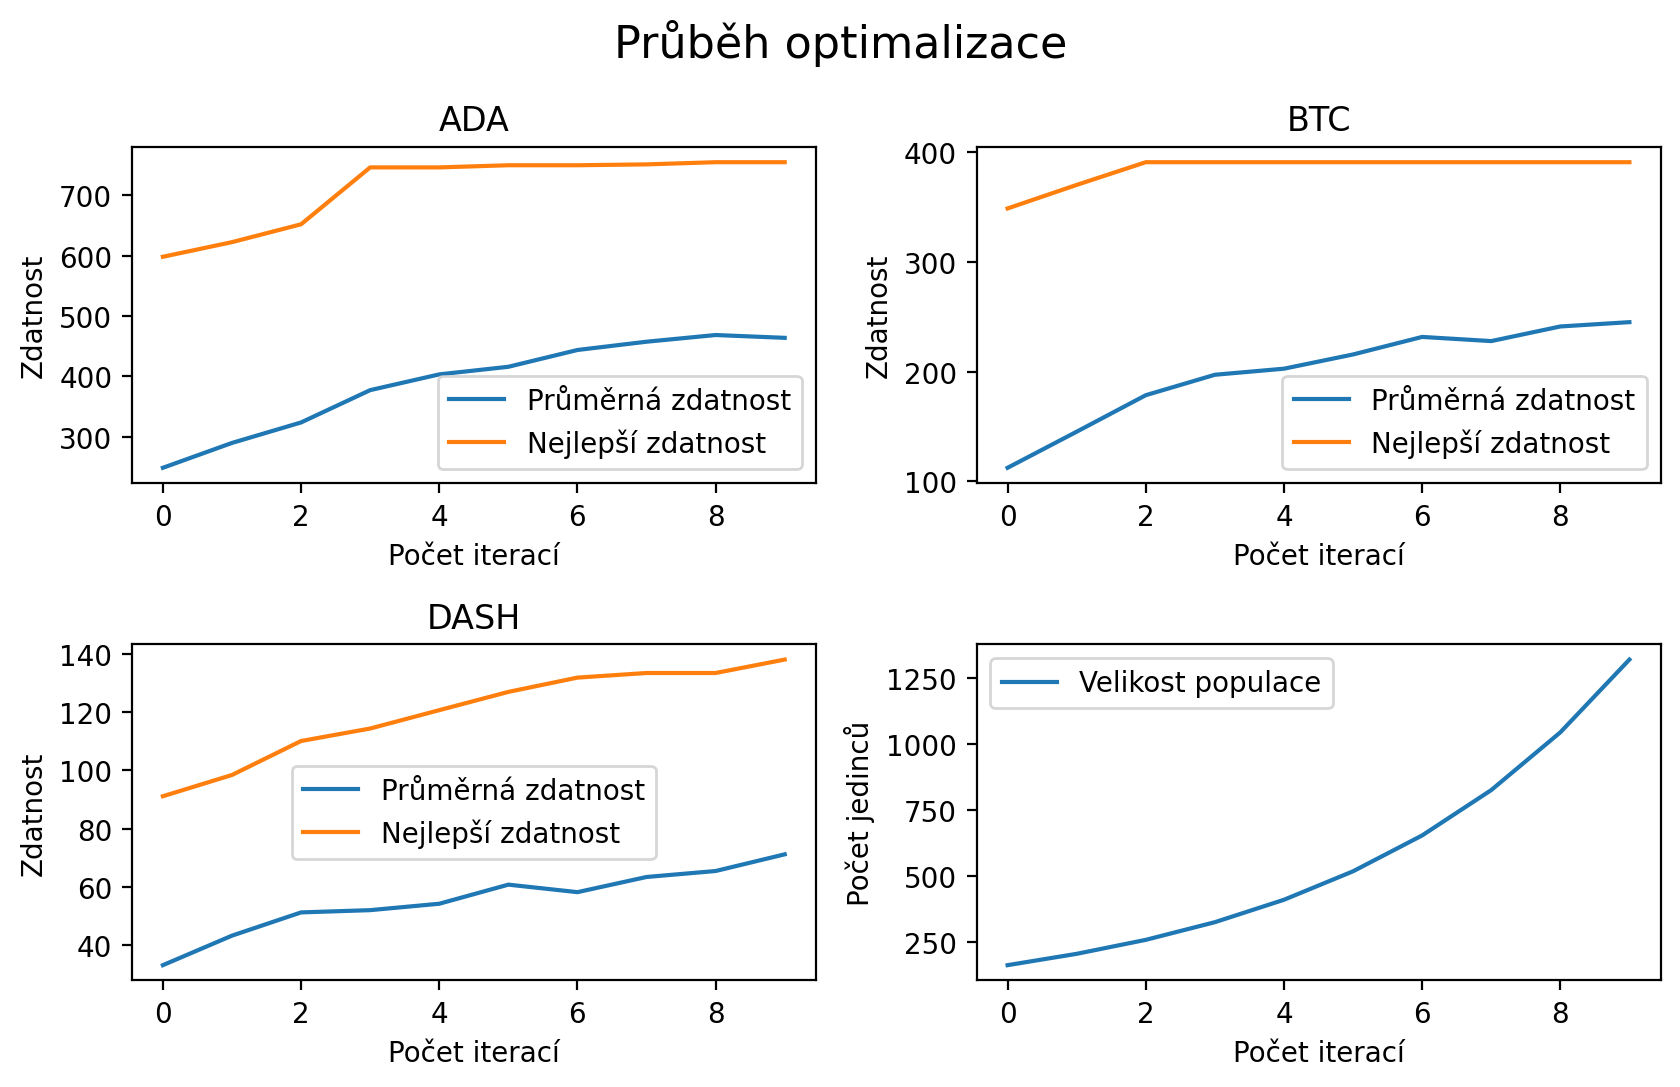
\includegraphics[scale=0.55]{img/genetic-algorithm-white-box-progress.png}}
\caption{Průběh optimalizace white-box testování genetického algoritmu}
\label{fig:genetic:algorithm:white:box:optimization:progress}
\end{figure}

\begin{table}[!htbp]
\centering
\caption[Výsledky white-box testování genetického algoritmu]{~Výsledky white-box testování genetického algoritmu}
\label{tab:genetic:algorithm:white:box:results}
{%
\begin{tabular}{|l|c|c|c|}
\hline
\multicolumn{1}{|c|}{\textbf{Měna}} &
  \textbf{\begin{tabular}[c]{@{}c@{}}Rozdíl hodnot\\ optimalizačního kritéria (\%)\end{tabular}} &
  \textbf{Doba trvání (s)} &
  \textbf{Zrychlení} \\ \hline
ADA  & 0,0 & 95,1  & 25,1 \\ \hline
BTC  & 0,0 & 121,1 & 20,4 \\ \hline
DASH & 0,0 & 75,9  & 22,1 \\ \hline
\end{tabular}%
}
\end{table}

Nakonec bylo provedeno black-box testování.
Výsledky jsou vidět v tabulce \ref{tab:genetic:algorithm:black:box:results}.
Optimální stav byl nalezen pro 4 ze 7 měn.
V případě SOL a XRP byly nalezené stavy o méně než \mbox{\(-1\) \%} horší než nejlepší a pro ETH o \mbox{\(-4,4\) \%}.
Celkově byly nalezeny velmi dobré konfigurace v přiměřeně krátkém čase.

\begin{table}[!htbp]
\centering
\caption[Výsledky black-box testování genetického algoritmu]{~Výsledky black-box testování genetického algoritmu}
\label{tab:genetic:algorithm:black:box:results}
{%
\begin{tabular}{|l|c|c|c|}
\hline
\multicolumn{1}{|c|}{\textbf{Měna}} &
  \textbf{\begin{tabular}[c]{@{}c@{}}Rozdíl hodnot\\ optimalizačního kritéria (\%)\end{tabular}} &
  \textbf{Doba trvání (s)} &
  \textbf{Zrychlení} \\ \hline
DOGE & 0,0  & 72,5  & 22,1 \\ \hline
ETH  & \(-4,4\) & 104,6 & 22,9 \\ \hline
LTC  & 0,0  & 98,4  & 21,5 \\ \hline
SOL  & \(-0,8\) & 50,1  & 24,3 \\ \hline
XLM  & 0,0  & 90,0  & 22,0 \\ \hline
XRP  & \(-0,3\) & 89,9  & 22,8 \\ \hline
ZRX  & 0,0  & 79,3  & 21,6 \\ \hline
\end{tabular}%
}
\end{table}

\section{Simulované ochlazování}
Soubor \texttt{settings.json} byl rozšířen o informace o optimalizátoru jako je počáteční a minimalní teplota, použitý rozvrh ochlazování a equilibrium.
Průběh optimalizace byl uložen do souboru \texttt{progress.csv}.
Obsahuje informace o hodnotě aktuální teploty, aktuálního stavu, nejlepšího stavu a průměrného prahu přijetí horšího stavu.
Při přijetí horšího stavu se zaznamená prahová hodnota, na základě které bylo rozhodnuto o jeho přijetí, pro každou iteraci je vypočten jejich průměr.
Měl by klesat s teplotou a je to další údaj, který může pomoci při ladění parametrů algoritmu.
Ukázku rozšíření logu lze vidět \ref{lst:simulated:annealing:log}.

\begin{lstlisting}[caption={~Rozšíření logu pro simulované ochlazování},label={lst:simulated:annealing:log},captionpos=t,abovecaptionskip=-\medskipamount,belowcaptionskip=\medskipamount]
it: 0, temperature: 94, curr value: 230.451, best value: 592.883
it: 1, temperature: 55.5179, curr value: 312.835, best value: 592.883
it: 2, temperature: 44.7915, curr value: 206.282, best value: 592.883
\end{lstlisting}

\subsection{Experimenty}
Sady měn pro white-box a black-box testování zůstaly stejné jako u předchozích experimentů.
Nejprve byly provedeny experimenty ke zjištění vhodného rozvrhu ochlazování, z nichž vynikla implementace třídy \texttt{basic\_cooler}.
Nepřebírá žádný parametr rozkladu a je závislá pouze na počáteční teplotě a aktuální iteraci.

% Začít s 2 skupinami vhodných nastavení
Pro výpočet počtu pokusů o změnu aktuálního stavu byla použita třída \texttt{fixed\_equilibrium}.
Po několika počátečních experimentech se sada rozdělila do 2 skupin, pro které dobře fungovala 2 různá nastavení.
Pro 1. skupinu skládající se z měn ADA a BTC byly hodnoty parametrů: počáteční teplota 128, minimální teplota 26 a počet pokusů 64 a pro 2. skupinu, která zahrnovala pouze DASH, bylo nastavení: počáteční teplota 54, minimální teplota 8 a počet pokusů 16.
Při použití nastavení 1. skupiny pro 2. DASH nedosáhl intenzifikační fáze a při opačném použití nastala intenzifikační fáze u 1. skupiny příliš brzy.

Jelikož byly rozsahy vhodných hodnot parametrů příliš daleko od sebe, byla navržena nová dynamičtější implementace equilibria  \texttt{temperature\_based\_equilibrium} založená na aktuální teplotě.
Počet pokusů vypočítá vynásobením aktuální teploty koeficientem.
Implementace umožnila snížení počtu pokusů s teplotou a tím spojení obou nastavení parametrů.

Nejlepší nalezené nastavení parametrů pro sadu white-box je uvedeno v tabulce \ref{tab:simulated:annealing:setting}.
Hodnota počáteční teploty je velmi blízká hodnotě vhodné pro 1. skupinu a hodnota minimální teploty zase hodnotě teploty vhodné pro 2. skupinu.
Počet pokusů je o 20 \% nižší než aktuální teplota, začíná tedy na 75 pokusech a končí na 10.
Rozsah změn generátoru náhodných období byl nastaven na 10 z výchozí hodnoty 1, jinak byl počet velikostí a úrovní, které lze změnit, ponechán na výchozí minimum.

\begin{table}[!htbp]
\centering
\caption[Nejlepší nalezené nastavení pro sadu white-box pro simulované ochlazování]{~Nejlepší nalezené nastavení pro sadu white-box pro simulované ochlazování}
\label{tab:simulated:annealing:setting}
\resizebox{\textwidth}{!}{%
\begin{tabular}{|c|c|c|c|c|c|}
\hline
\textbf{\begin{tabular}[c]{@{}c@{}}Počáteční\\ teplota\end{tabular}} &
  \textbf{\begin{tabular}[c]{@{}c@{}}Minimální\\ teplota\end{tabular}} &
  \textbf{\begin{tabular}[c]{@{}c@{}}Koeficient equilibria\\ založeném na teplotě (\%)\end{tabular}} &
  \textbf{\begin{tabular}[c]{@{}c@{}}Rozsah změny\\ období\end{tabular}} &
  \textbf{\begin{tabular}[c]{@{}c@{}}Počet změn\\ nákupních úrovní\end{tabular}} &
  \textbf{\begin{tabular}[c]{@{}c@{}}Počet změn\\ nákupních velikostí\end{tabular}} \\ \hline
94 &
  12 &
  \(-20\) &
  10 &
  2 &
  1 \\ \hline
\end{tabular}%
}
\end{table}

Průběh optimalizace white-box testování je vidět na grafu \ref{fig:simulated:annealing:white:box:optimization:progress}.
V případě ADA dochází ke krátkému období diverzifikace, které rychle přechází do fáze intenzifikace.
U BTC je přechod pomalejší a u DASH lze vypozorovat, že dochází k výraznější diverzifikační fázi.
Individuálně lze tedy nalézt lepší hodnoty parametrů, ale i přesto se podařilo konvergovat ke globálním optimům, což lze vidět v tabulce \ref{tab:simulated:annealing:white:box:results}.
Počet iterací je řádově vyšší než u genetického algoritmu, ale trvají mnohem kratší dobu.
Průměrné zrychlení je \textbf{11,4} oproti hrubé síle a čas optimalizace se pohybuje mezi \textbf{2,5--3,9} minut.
Je tedy asi \textbf{2krát} pomalejší než genetický algoritmus.
Nicméně ve výsledcích testování black-box byl genetický algoritmus překonán, protože byly nalezeny optimální konfigurace pro všechny měny v sadě (viz \ref{tab:simulated:annealing:black:box:results}).

\begin{figure}[!htbp]
\centerline{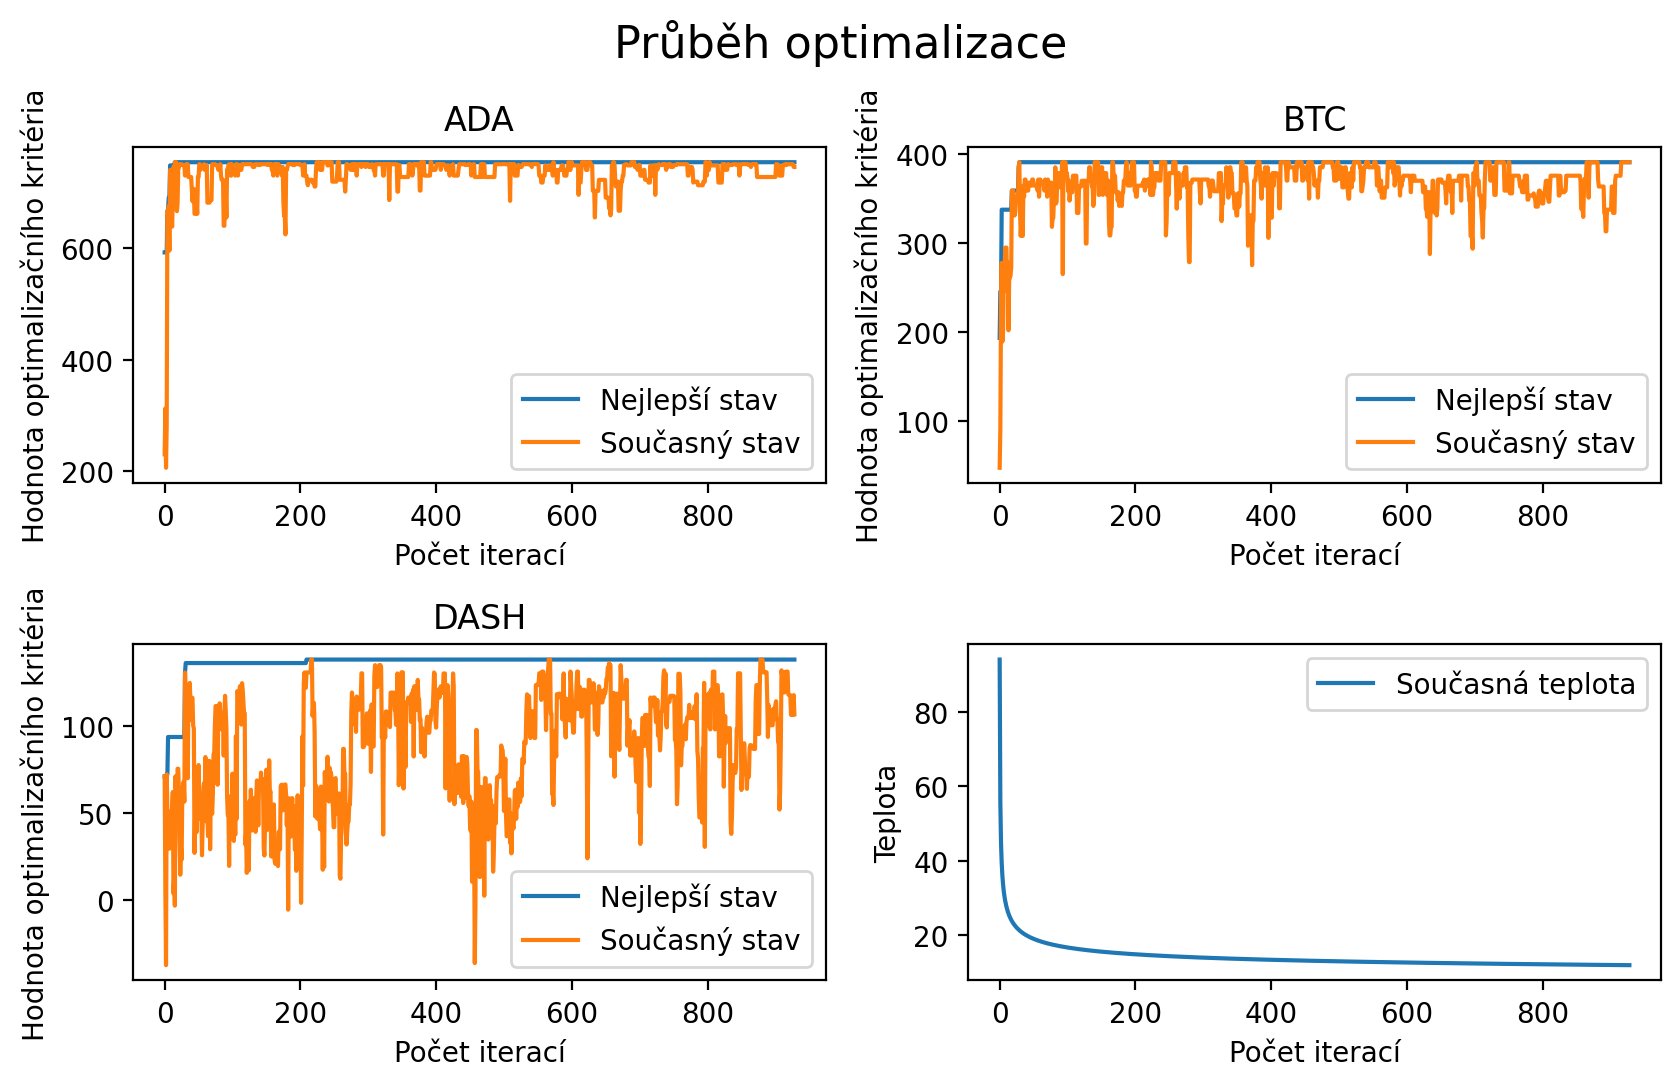
\includegraphics[scale=0.55]{img/simulated-annealing-white-box-progress.png}}
\caption{Průběh optimalizace white-box testování simulovaného ochlazování}
\label{fig:simulated:annealing:white:box:optimization:progress}
\end{figure}

% Please add the following required packages to your document preamble:
% \usepackage{graphicx}
\begin{table}[!htbp]
\centering
\caption[Výsledky white-box testování simulovaného ochlazování]{~Výsledky white-box testování simulovaného ochlazování}
\label{tab:simulated:annealing:white:box:results}
{%
\begin{tabular}{|l|c|c|c|}
\hline
\multicolumn{1}{|c|}{\textbf{Měna}} &
  \textbf{\begin{tabular}[c]{@{}c@{}}Rozdíl hodnot\\ optimalizačního kritéria (\%)\end{tabular}} &
  \textbf{Doba trvání (s)} &
  \textbf{Zrychlení} \\ \hline
ADA  & 0,0 & 191,5 & 12,4 \\ \hline
BTC  & 0,0 & 233,3 & 10,6 \\ \hline
DASH & 0,0 & 151,2 & 11,1 \\ \hline
\end{tabular}%
}
\end{table}

\begin{table}[!htbp]
\centering
\caption[Výsledky black-box testování simulovaného ochlazování]{~Výsledky black-box testování simulovaného ochlazování}
\label{tab:simulated:annealing:black:box:results}
{%
\begin{tabular}{|l|c|c|c|}
\hline
\multicolumn{1}{|c|}{\textbf{Měna}} &
  \textbf{\begin{tabular}[c]{@{}c@{}}Rozdíl hodnot\\ optimalizačního kritéria (\%)\end{tabular}} &
  \textbf{Doba trvání (s)} &
  \textbf{Zrychlení} \\ \hline
DOGE & 0,0 & 159,7 & 10,0 \\ \hline
ETH  & 0,0 & 192,5 & 12,5 \\ \hline
LTC  & 0,0 & 177,2 & 12,0 \\ \hline
SOL  & 0,0 & 86,9  & 14,0 \\ \hline
XLM  & 0,0 & 163,8 & 12,1 \\ \hline
XRP  & 0,0 & 161,2 & 12,7 \\ \hline
ZRX  & 0,0 & 133,8 & 12,8 \\ \hline
\end{tabular}%
}
\end{table}

\section{Tabu prohledávání}
Do souboru \texttt{settings.json} byly přidány informace o nastavení optimalizátoru: počet iterací tabu lhůty, velikost sousedství a kritérium ukončení.
Průběh optimalizace byl uložen do souboru \texttt{progress.csv} a obsahoval informace o hodnotě optimalizačního kritéria aktuálního a nejlepšího stavu a velikosti krátkodobé paměti.
Log byl také náležitě doplněn (viz \ref{lst:tabu:search:log}).

\begin{lstlisting}[caption={~Rozšíření logu pro tabu prohledávání},label={lst:tabu:search:log},captionpos=t,abovecaptionskip=-\medskipamount,belowcaptionskip=\medskipamount]
it: 10, best value: 27.2462, curr value: 27.2462, tabu list size: 11
it: 11, best value: 37.0617, curr value: 37.0617, tabu list size: 12
it: 12, best value: 52.0412, curr value: 52.0412, tabu list size: 13
\end{lstlisting}

\subsection{Experimenty}
Při hledání vhodného nastavení byly nejdůlžitější hodnoty 2 parametrů, tabu lhůty, která udává počet iterací, během kterých je atribut označen jako tabu, a velikost sousedství, který udává počet sousedů, kteří jsou prohledáni během jedné iterace.
Posledním parametrem bylo kritérium ukončení, které bylo implementováno pomocí \texttt{itation\_based\_termination}.
Všechny hodnoty parametrů byly pevně dané, takže se během optimalizace neměnily.

Pokud je hodnota tabu lhůty příliš nízká, dostane se do lokálního optima, z kterého se ji nepodaří uniknout a zůstane ve fázi vytěžování.
Na druhou stranu, pokud je příliš vysoká, heuristika se nemůže vrátit do slibné oblasti a převažuje fáze průzkumu.
Když je velikost sousedství příliš malé, pohybuje se heuristika rychleji skrze stavový prostor a okolí aktuálního stavu zůstává neprozkoumané.
Naopak pokud je příliš velké, prozkoumává podobné konfigurace, pohybuje se pomalu a zůstává ve stejné oblasti stavového prostoru.
Jinými slovy, tabu lhůta pomáhá držet směr a velikost sousedství udává velikost kroku.

Nejlepší parametry nalezené pro sadu white-box jsou uvedeny v tabulce \ref{tab:tabu:search:setting}.
Nastavení náhodných generátorů stavového prostoru bylo ponecháno stejné jako u předchozí heuristiky.
Z grafu \ref{fig:tabu:search:white:box:optimization:progress} je vidět, že v prvních 20 iteracích došlo k rychlé konvergenci.
Dále si lze všimnout, že když se heuristika začne přesouvat z fáze vytěžování do fáze průzkumu, tak se hodnota optimalizačního kritéria aktuálního stavu začne vzdalovat tomu nejlepšímu.
Například v případě BTC se začne vzdalovat od nejlepšího stavu kolem 20. iterace a vrací se až v 50. iteraci, kdy najde lepší konfiguraci.

\begin{table}[!htbp]
\centering
\caption[Nejlepší nalezené nastavení pro sadu white-box pro tabu prohledávání]{~Nejlepší nalezené nastavení pro sadu white-box pro tabu prohledávání}
\label{tab:tabu:search:setting}
\resizebox{\textwidth}{!}{%
\begin{tabular}{|c|c|c|c|c|c|}
\hline
\textbf{Tabu lhůta} &
  \textbf{Velikost sousedství} &
  \textbf{Počet iterací} &
  \textbf{\begin{tabular}[c]{@{}c@{}}Rozsah změny\\ období\end{tabular}} &
  \textbf{\begin{tabular}[c]{@{}c@{}}Počet změn\\ nákupních úrovní\end{tabular}} &
  \textbf{\begin{tabular}[c]{@{}c@{}}Počet změn\\ nákupních velikostí\end{tabular}} \\ \hline
32 &
  128 &
  128 &
  10 &
  2 &
  1 \\ \hline
\end{tabular}%
}
\end{table}

Velikost paměti téměř vždy dosáhne hodnotě blízké své maximální kapacitě, která je rovna tabu lhůtě.
Pokud je stejný atribut zapamatován vícekrát po sobě, velikost paměti se sníží.
Tah aktuálního stavu může být tabu, jelikož se musí aktuální stav každou iteraci změnit.

Průměrné zrychlení oproti hrubé síle pro sadu white-box je \textbf{9,5}, což je o trochu pomalejší než simulované ochlazování.
Doba výpočtu se pohybuje v rozmezí \textbf{3,1-4,4} minuty.
Opět bylo dosaženo globálního optima pro všechny měny.
Při použití na vzorky ze sady black-box bylo dosaženo 3 ze 7 globálních optim.
Rozdíl mezi globálním optimem byl nižší než \(-2\) \% ve 3 případech.
Nejvýznamnější rozdíl byl \(-9,8\) \%, což je 2krát horší výsledek než nejhorší výsledek při použití genetického algoritmu.

\begin{figure}[!htbp]
\centerline{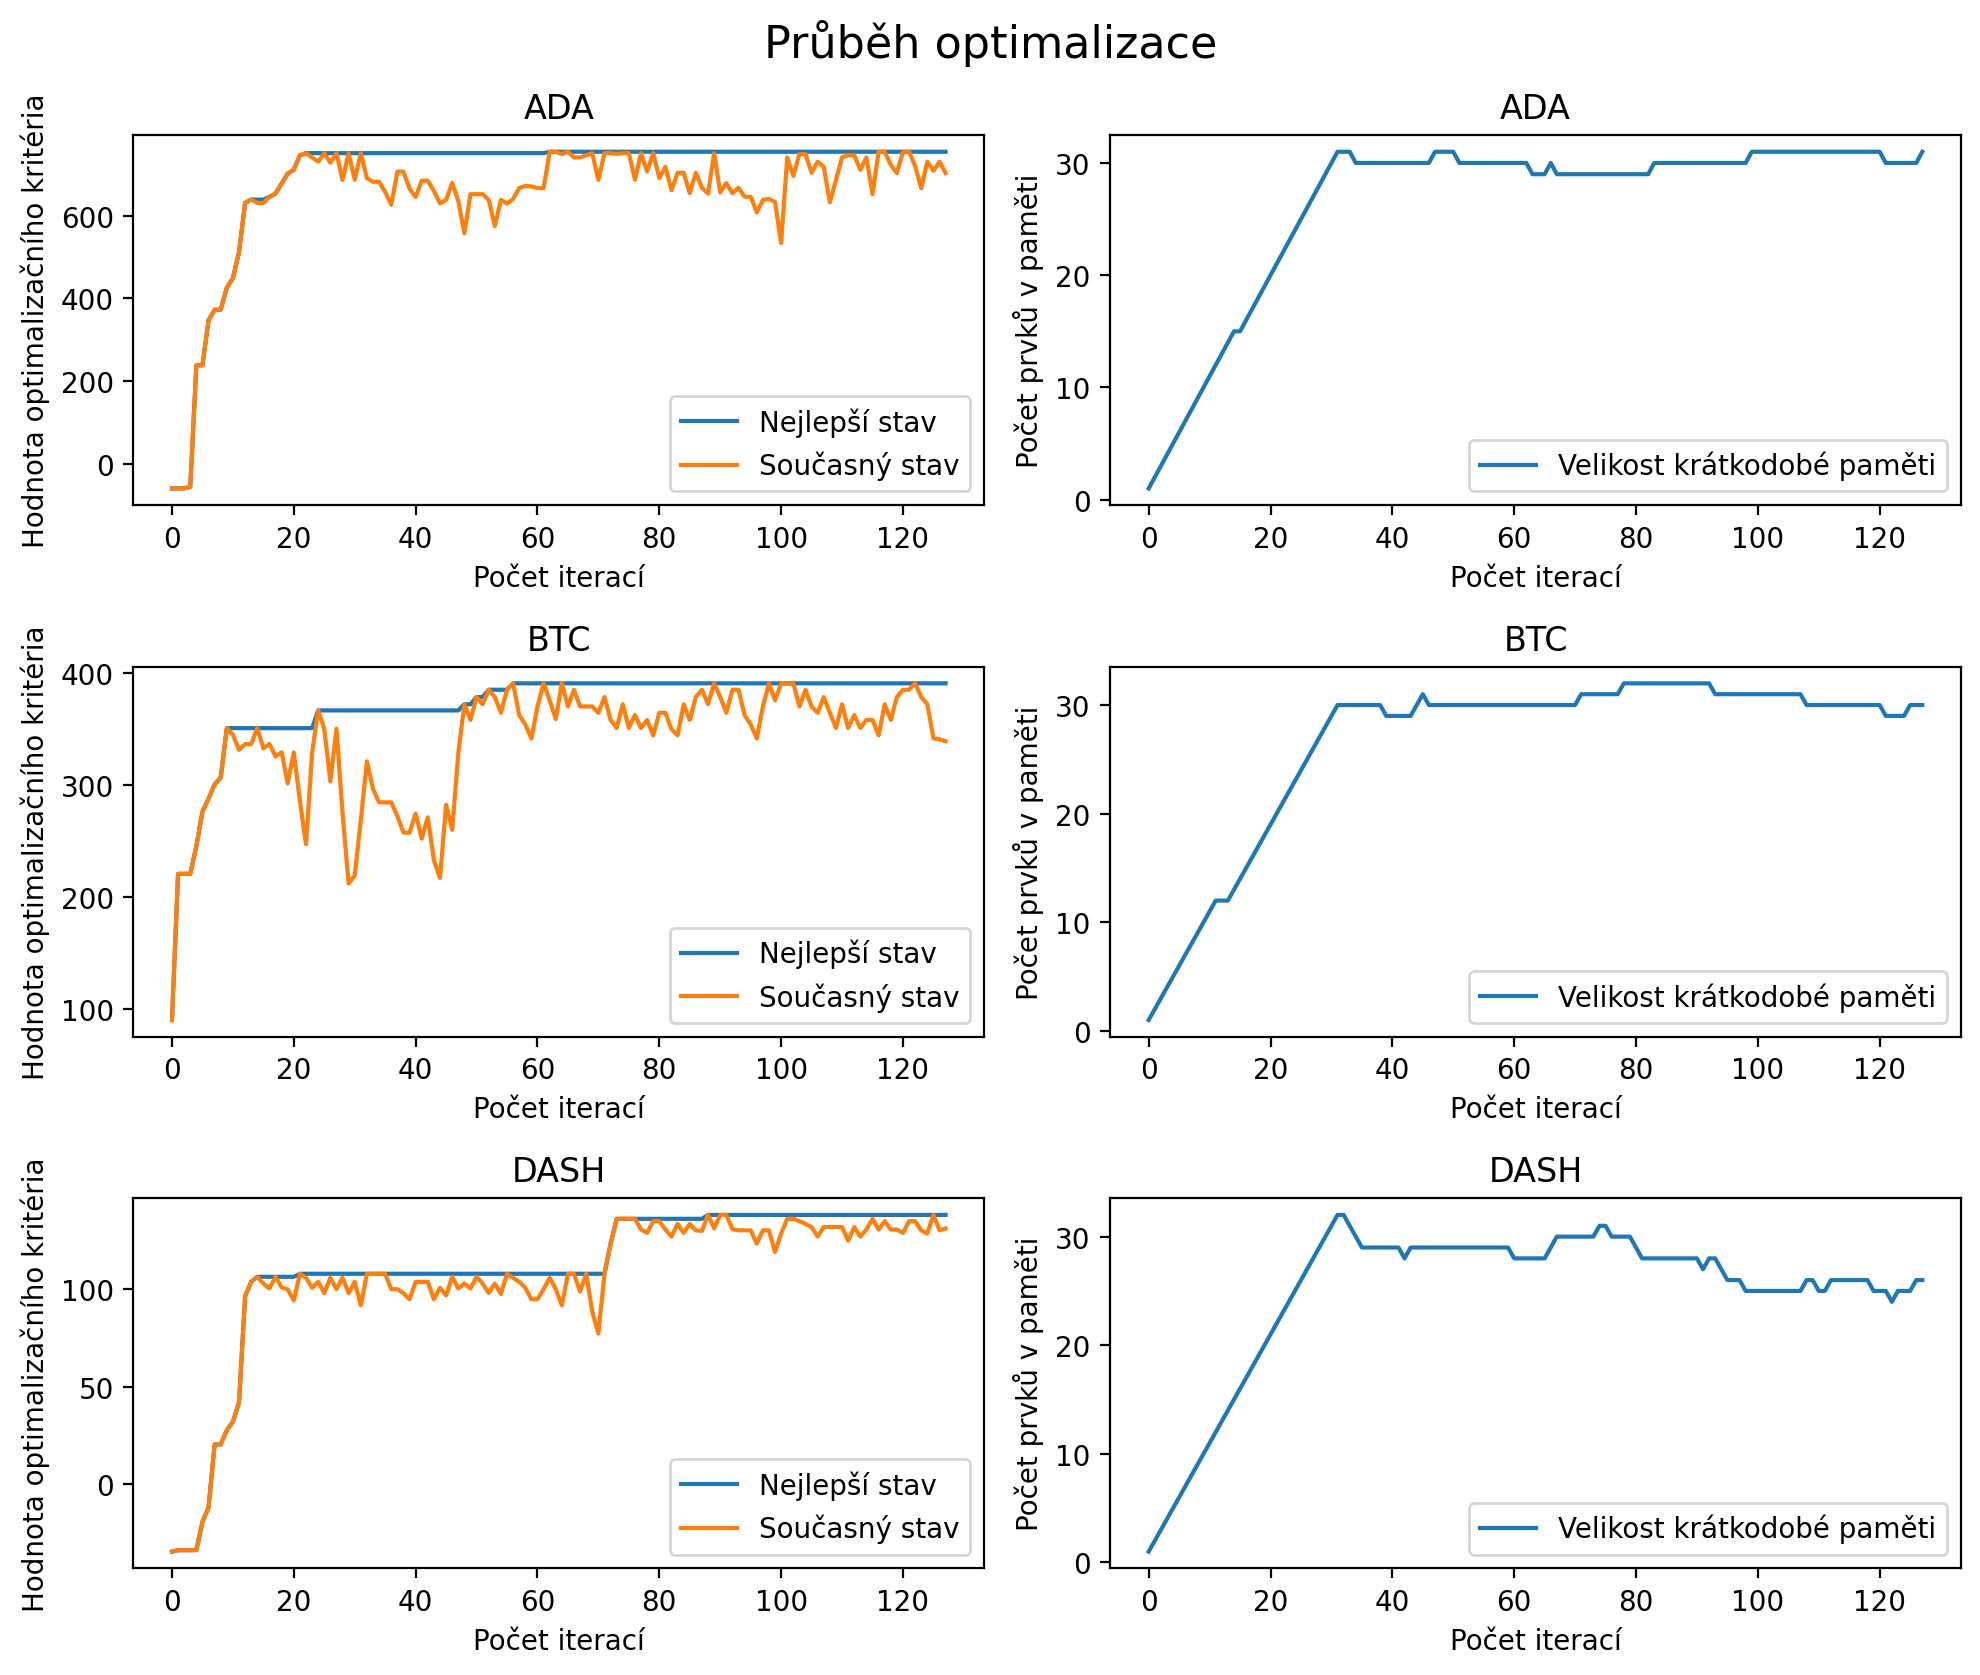
\includegraphics[scale=0.55]{img/tabu-search-white-box-progress.png}}
\caption{Průběh optimalizace white-box testování tabu prohledávání}
\label{fig:tabu:search:white:box:optimization:progress}
\end{figure}

\begin{table}[!htbp]
\centering
\caption[Výsledky white-box testování simulovaného ochlazování]{~Výsledky white-box testování simulovaného ochlazování}
\label{tab:tabu:search:white:box:results}
{%
\begin{tabular}{|l|c|c|c|}
\hline
\multicolumn{1}{|c|}{\textbf{Měna}} &
  \textbf{\begin{tabular}[c]{@{}c@{}}Rozdíl hodnot\\ optimalizačního kritéria (\%)\end{tabular}} &
  \textbf{Doba trvání (s)} &
  \textbf{Zrychlení} \\ \hline
ADA  & 0,0 & 241,1 & 9,9 \\ \hline
BTC  & 0,0 & 260,8 & 9,5 \\ \hline
DASH & 0,0 & 184,3 & 9,1 \\ \hline
\end{tabular}%
}
\end{table}

\begin{table}[!htbp]
\centering
\caption[Výsledky black-box testování tabu prohledávání]{~Výsledky black-box testování tabu prohledávání}
\label{tab:tabu:search:black:box:results}
{%
\begin{tabular}{|l|c|c|c|}
\hline
\multicolumn{1}{|c|}{\textbf{Měna}} &
  \textbf{\begin{tabular}[c]{@{}c@{}}Rozdíl hodnot\\ optimalizačního kritéria (\%)\end{tabular}} &
  \textbf{Doba trvání (s)} &
  \textbf{Zrychlení} \\ \hline
DOGE & 0,0  & 158,8 & 10,1 \\ \hline
ETH  & 0,0  & 272,4 & 8,8  \\ \hline
LTC  & 0,0  & 249,4 & 8,5  \\ \hline
SOL  & -0,8 & 91,2  & 13,4 \\ \hline
XLM  & -9,8 & 207,1 & 9,6  \\ \hline
XRP  & -1,7 & 227,5 & 9,0  \\ \hline
ZRX  & -1,4 & 227,9 & 7,5  \\ \hline
\end{tabular}%
}
\end{table}